%%% File encoding: UTF-8
%%% äöüÄÖÜß  <-- keine deutschen Umlaute hier? UTF-faehigen Editor verwenden!

\documentclass[bachelor,german]{hgbthesis}
% Zulässige Class Options: 
%   Typ der Arbeit: diplom, master (default), bachelor, praktikum 
%   Hauptsprache: german (default), english
%%%----------------------------------------------------------

\RequirePackage[utf8]{inputenc}		% Bei der Verw. von lualatex oder xelatex entfernen!

\graphicspath{{images/}}    % Abbildungsverzeichnis
\logofile{beuth_basis}				% Name des Logo-PDFs in images/ (\logofile{}, wenn kein Logo gewünscht)
\bibliography{literatur}  	% Name der Biblatex-Literaturdatei (.bib)

%%%----------------------------------------------------------
% Angaben für die Titelei (Titelseite, Erklärung etc.)
%%%----------------------------------------------------------

%%% Einträge für ALLE Arbeiten: -----------------------------
\title{Simulation von Brandszenarien zur Ermittlung von Sprinklerauslösezeiten mit FDS im Vergleich zur VDI 6019 Blatt 1}
\author{Niklas A. Wittkämper}
\studiengang{der Beuth Hochschule für Technik}
\studienort{Berlin}
\abgabedatum{2019}{12}{17}	% {YYYY}{MM}{DD}

%%% Zusätzlich für eine Bachelorarbeit: ---------------------
\nummer{849934}   % Stud-ID, z.B. 1310238045-A  
% (A = 1. Bachelorarbeit)
\semester{Sommersemester 2019} 
\gegenstand{Fachbereich} 
\betreuer{Prüfungskommission: Prof. Dr. Finke und Dipl.-Ing. Peter Thiel} % oder \betreuerin{..}

%%% Restriktive Lizenformel anstatt CC (nur für Typ master) -
%\strictlicense

%%%----------------------------------------------------------
\begin{document}
%%%----------------------------------------------------------
\addtocontents{toc}{\vspace{-3ex}}
%%%----------------------------------------------------------
\frontmatter                    % Titelei (röm. Seitenzahlen)
%%%----------------------------------------------------------
\newgeometry{hoffset=-0.04cm, textwidth=16cm, voffset=3cm, textheight=25cm}
\maketitle
\restoregeometry
\includepdf[offset=-0.5cm -2cm,noautoscale=true,addtotoc={1,chapter,1,Aufgabenstellung,1},pagecommand={\thispagestyle{plain}}]{images/Aufgabenstellung.pdf}

\begin{onehalfspace}
\setlength{\cftbeforetoctitleskip}{1em}
\tableofcontents

%\chapter{Vorwort}

 % Optional. Ggf. weglassen

\chapter{Kurzfassung}

In der vorliegenden Arbeit werden Sprinklerszenarien mit der CFD-Software FDS (Fire Dynamics Simulator) simuliert. Das Simulationsmodell ist ein Raum mit unendlicher Decke und offenen Seiten. Es wird betrachtet, wie verschiedene Parameter (Raumhöhe, Brandintensitätskoeffizient, RTI) Einfluss auf die Sprinklerauslösezeit nehmen. Der Brand wird mit quadratischer Zunahme der Wärmefreisetzungrate und Brandfläche simuliert. 
Bestehende Literatur wird betrachtet und verschiedene Rechenansätze werden angeführt. Daten aus FDS werden visuell ausgewertet und interpretiert. 
Die Ergebnisse werden mit den Tabellenwerten der VDI 6019:2006 Blatt 1 und dem SFPE Handbook of Fire Protection Engineering, 3rd Edition verglichen. Es stellt sich heraus, dass die VDI~6019 nicht mehr dem derzeitigen Wissenschaftsstand widerspiegelt. Nach einer Untersuchung der Kennwerte in FDS und dem Vergleich zu Literaturquellen wird ermittelt, dass ein C-Faktor von 0~(m/s)$^{0,5}$ die Sprinklerauslösezeiten am besten vorhersagt. Übereinstimmungen der Auslösezeiten zwischen Simulation und Berechnung sind sehr hoch, vor allem bei niedrigen Nennöffnungstemperaturen.  










		
%\chapter{Abstract}

\begin{english} %switch to English language rules
This should be a 1-page (maximum) summary of your work in English.
%und hier geht dann das Abstract weiter...
\end{english}

Im englischen Abstract sollte inhaltlich das Gleiche
stehen wie in der deutschen Kurzfassung. Versuchen Sie daher, die
Kurzfassung prä\-zise umzusetzen, ohne aber dabei Wort für Wort zu
übersetzen. Beachten Sie bei der Übersetzung, dass gewisse
Redewendungen aus dem Deutschen im Englischen kein Pendant haben
oder völlig anders formuliert werden müssen und dass die
Satzstellung im Englischen sich (bekanntlich) vom Deutschen stark
unterscheidet (mehr dazu in Abschn.\ \ref{sec:englisch}). Es
empfiehlt sich übrigens -- auch bei höchstem Vertrauen in die
persönlichen Englischkenntnisse -- eine kundige Person für das
"`proof reading"' zu engagieren.

Die richtige Übersetzung für "`Diplomarbeit"' ist übrigens
schlicht \emph{thesis}, allenfalls  "`diploma thesis"' oder "`Master's thesis"', 
auf keinen Fall aber "`diploma work"' oder gar "`dissertation"'. 
Für "`Bachelorarbeit"' ist wohl "`Bachelor thesis"' die passende Übersetzung. 

Übrigens sollte für diesen Abschnitt die \emph{Spracheinstellung} in \latex\ von Deutsch
auf Englisch umgeschaltet werden, um die richtige Form der
Silbentrennung zu erhalten, die richtigen Anführungszeichen müssen allerdings selbst gesetzt werden %
(s.\ dazu die Abschnitte \ref{sec:sprachumschaltung} %
und \ref{sec:anfuehrungszeichen}).
			
\printnomenclature
%%%----------------------------------------------------------
\mainmatter  % Hauptteil (ab hier arab. Seitenzahlen)
%%%----------------------------------------------------------

\chapter{Einleitung}
\label{cha:Einleitung}

Der Brandschutz nimmt in der Gebäudetechnik einen essentiellen Teil ein. Beim vorbeugenden Brandschutz wird durch baulichen, anlagentechnischen und organisatorischen Brandschutz versucht, die potentielle Gefährdung für Mensch und Leben in Gebäuden bei einem Brand zu minimieren. Das Risiko für den Menschen geht hierbei meist durch die gefährliche Rauchentwicklung aus. 
So liegt die Quote der Todesfälle durch Rauchvergiftung und Erstickung bei Bränden in Gebäuden bei 90 \%. Die Wichtigkeit, mithilfe des anlagentechnischen Brandschutzes das Risiko für den Menschen zu minimieren, steht somit außer Frage. Entrauchungsanlagen sorgen dafür, dass der beim Brand entstandene Rauch aus dem Gebäude geleitet wird und Flucht- und Rettungswege gesichert werden. 
Zusätzlich wird oftmals vorgeschrieben, automatische Sprinklersysteme vorzusehen. Löschwasser begrenzt nach der Aktivierung durch gleichmäßiges Verteilen die Brandausbreitung und Rauchfreisetzung. Eine weitere grundsätzliche Aufgabe ist die nachgeschaltete Alarmierung der Feuerwehr nach der Auslösung. Hier ist es also wichtig, dass das Sprinklersystem schnell und zuverlässig auslöst. 

Heutzutage erforderten die Größe, Komplexität und Einzigartigkeit neuartiger Gebäude die Anwendung innovativer Methoden, um den brandschutztechnischen Nachweis, trotz Abweichungen von den bestehenden baurechtlichen Vorgaben, erbringen zu können. 
Dies erfolgt des Öfteren mithilfe von Computermodellen. Sogenannte CFD (Computational Fluid Dynamics)-Software benutzt numerische Methoden, um komplexe Strömungsmechanik simulieren zu können (wie \zB Entrauchungssimulationen). 

Um Entrauchungsanlagen richtig zu dimensionieren, ist es essentiell, die Sprinklerauslösezeiten so genau wie möglich vorhersagen zu können. Da die Sprinkleranlage das Feuer an der Ausbreitung verhindert, kann ausgesagt werden, wann der Brandherd eine bestimmte Leistung erreicht und damit auch wieviel Rauch bis zu diesem Zeitpunkt freigesetzt wurde und wieviel Rauch nachfolgend noch freigesetzt wird. Längere Sprinklerauslösezeiten führen also zu einer größeren Brandausbreitung als kürzere Auslösezeiten. Dies kann schlussendlich erhebliche Auswirkungen auf die Größe der Entrauchungsanlage haben. Die VDI-Richtlinie 6019:2006 "`Ingenieurmethoden zur Auslegung von Entrauchungsanlagen"' beschreibt diesen Sachverhalt.

In dieser Arbeit wird untersucht, wie präzise das Simulationsprogramm FDS (Fire Dynamics Simulator) Sprinklerauslösezeiten vorhersagen kann. Dies beinhaltet den Vergleich der Ergebnisse mit der VDI 6019:2006 und dem SFPE Handbook 3rd Ed. In FDS wird ein realistischer Brandherd in einem Raum mit offener Decke simuliert. Verschiedene Kennwerte der Sprinklerköpfe werden außerdem untersucht. 

Diese Arbeit wurde im Unternehmen ROM Technik in der Abteilung Forschung und Entwicklung im wärme- und strömungstechnischen Labor in Hamburg angefertigt.

%%\SuperPar In dieser Arbeit wird nach der Aufgabenstellung zunächst im Grundlagenkapitel auf die verschiedenen Einflussfaktoren im Bezug auf Sprinklerauslösezeiten eingegangen. Anschließend beschreibt der Hauptteil alle notwendigen Rechnungen und die Simulationssoftware FDS. Es wird auf das Simulationsmodell eingegangen, sowie alle Vorüberlegungen, die zum endgültigen Modell geführt haben. Darauf folgend werden alle Versuchsergebnisse vorgestellt und ausgewertet. Im Kapitel "`Fazit"' werden die Ergebnisse dieser Arbeit in die vorhandene Literatur eingeordnet und abschließende Gedanken zu finden sein. Im Anhang sind alle für die Simulationen benutzte Input-Dateien enthalten.

%\chapter{Grundlagen}
\label{cha:Grundlagen}
\section{Grundprinzip und Wärmetransport}
\label{sec:WaermeuebergaengeamSprinklerkopf}


Die Sprinklerkopfaktivierung läuft wie folgt ab: über dem Brandherd entsteht eine Rauchgassäule (nachfolgend Plume genannt). Der Rauch steigt auf und breitet sich unter der Decke aus. Hierbei wird Umgebungsluft in den Plume induziert. An der Decke breitet sich ein radialer Deckenstrahl aus (nachfolgend Ceiling Jet genannt), welcher am Sprinklerkopf vorbeiströmt. Die heiße Verbrennungsluft erhitzt das Auslöseelement und es kommt bei Erreichen der Auslösetemperatur zur Aktivierung. 
\begin{figure}
    \centering
    \includegraphics[trim=0 3.5cm 0cm 3cm,clip,width=0.8\textwidth]{images/PlumeCeilingJet.pdf}
    \caption{Plume und Ceiling Jet an unbegrenzter Decke \cite{SFPE5th}}
    \label{fig:PlumeUndJet}
\end{figure}
Abb. \ref{fig:PlumeUndJet} zeigt hierzu eine idealisierte Rauchgasausbreitung mit den Parametern $r$ und $H$. $r$ bezeichnet den horizontalen Abstand zwischen Brandherdmitte und Sprinklerkopf und $H$ den vertikalen Abstand zwischen Brandherdoberkante und Deckenunterkante.
Die grundsätzlichen Wärmetransportarten am Sprinklerkopf sind die Konvektion, Strahlung und Leitung (siehe Abb. \ref{fig:waermeuebergaenge}). Der bedeutendste Wärmetransport bei der Sprinkleraktivierung ist die Konvektion. Die Wärme des heißen Rauchgases geht an die Oberf"|läche des Auslöseelements über und erwärmt anschließend per Wärmeleitung die Flüssigkeit in der Glasampulle. 
Der spezifische Wärmestrom der Luft an die Glasampulle kann mit der Formel $\Dot{Q}/A=h \cdot (T_1 - T_2)$ beschrieben werden. Hierbei ist $h$ die Wärmeübergangszahl, $A$ die vom Fluid benetzte Oberf"|läche und $T_1$ und $T_2$ die Temperatur des Fluids, \bzw der Glasoberf"|läche. Für die Wärmeübergangszahl sind Parameter wie die Gasgeschwindigkeit und die verschiedenen Stoffwerte des Rauchgases von Interesse. 


Das Auslöseelement befindet sich in einem stetigen Strahlungsaustausch mit seiner Umgebung. Bei einem Feuer kann die Flammentemperatur mehrere tausend Grad betragen. Hierbei wird also das Glasfässchen über Wärmestrahlung vom Feuer erhitzt. Untersuchungen zeigen allerdings, dass im Anfangsstadium des Feuers die Wärmestrahlung vernachlässigt werden kann \cite[S. 1320]{SFPE5th}. Sie wird also weder bei der Berechnung noch bei der Simulation in Betracht gezogen. 

Als letzte Transportart ist die Wärmeleitung zwischen der Glasampulle und dem Sprinklerkopf zu beachten. Sie ist zumeist mit dem Wärmeleitfaktor C angegeben und wird in Kap. \ref{sec:CFaktor} weiterführend erklärt.

\begin{figure}
    \centering
    \includegraphics[trim=0 3cm 0cm 3cm,clip,width=0.7\textwidth]{images/Waermeuebergaenge.pdf}
    \caption{Wärmeübergänge am Sprinklerkopf \cite{SFPE5th}}
    \label{fig:waermeuebergaenge}
\end{figure}







\section{Sprinklerkopfaufbau und Kennwerte}
\label{sec:Sprinklerkennwerte}
\subsection{Aufbau des Sprinklerkopfes}
\label{sec:AufbauSprinkler}
Während die ersten Erwähnungen eines automatischen Sprinklersystems schon bis zu Leonardo da Vincis Zeiten zurückreichen \cite{WikiSprinkler}, gibt es den Sprinklerkopf in der Form wie wir ihn kennen erst seit 1890 \cite{Patent}. Seit dem ursprünglichen Patent hat sich am grundsätzlichen Aufbau nicht viel verändert. Die Hauptbestandteile eines Sprinklerkopfes sind in Abb. \ref{fig:AufbauSprinklerkopf} zu erkennen.
\begin{figure}
    \centering
    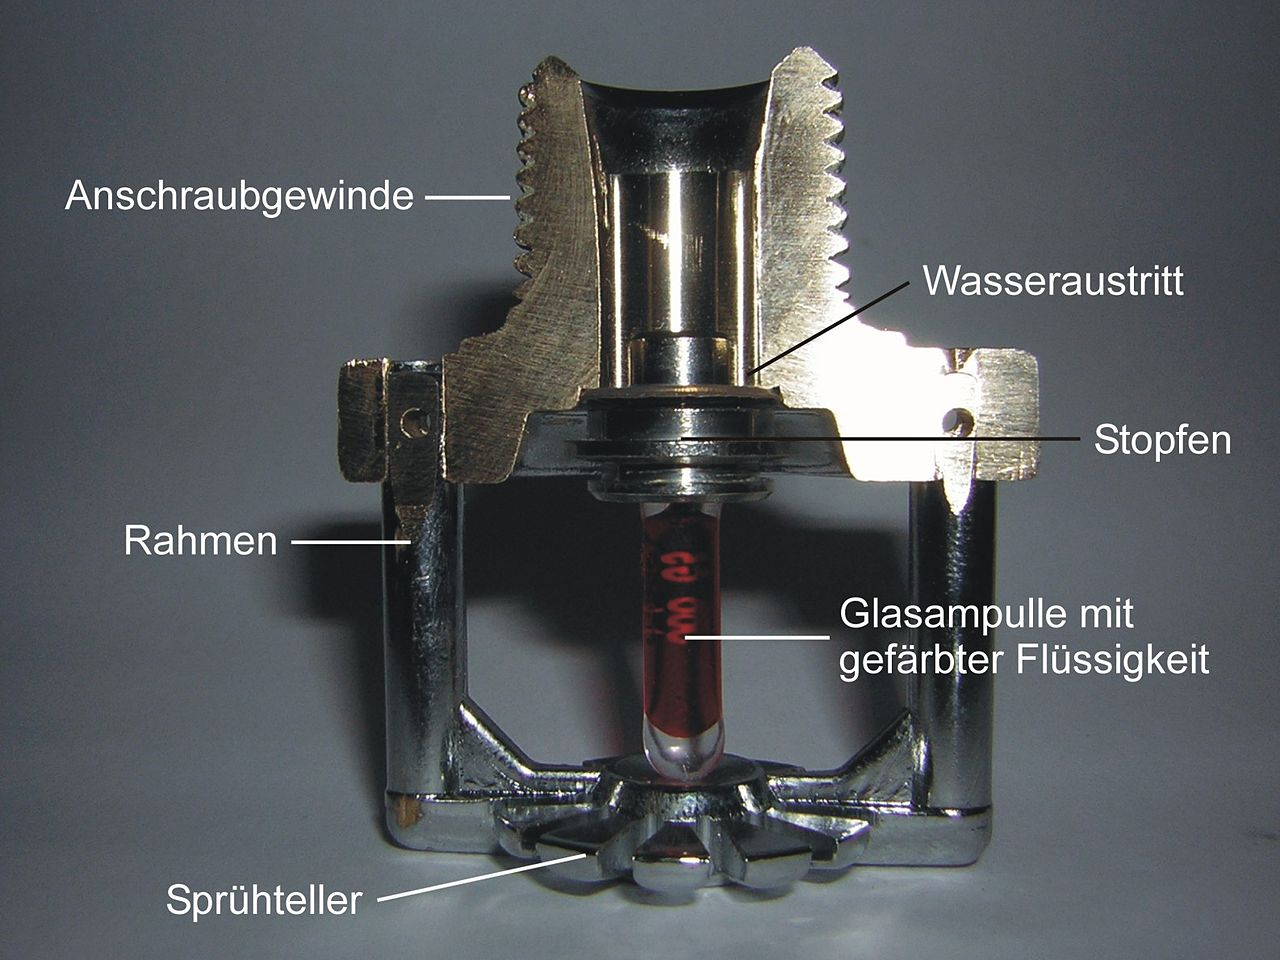
\includegraphics{images/sprinklerkopf.jpg}
    \caption{Aufbau Sprinklerkopf \cite{Sprinklerkopf}}
    \label{fig:AufbauSprinklerkopf}
\end{figure}
Unterschieden wird zwischen Glasfass- und Schmelzlot-Sprinklern. In dieser Arbeit wird auschließlich der gängigere Typ mit Glasfass betrachtet. Außerdem gibt es neben den hier betrachteten hängenden Sprinklerköpfen noch \zB Seitenwand- oder verdeckte Sprinklerköpfe.

Bei der Montage wird der Sprinklerkopf über das Anschraubgewinde mit der Sprinklerleitung verbunden. Nachdem die Sprinkleranlage mit Wasser befüllt wurde, ist der Sprinklerkopf funktionsfähig. Die Glasampulle drückt gegen den Stopfen und verhindert so ein Entweichen des Wassers. Im Brandfall dehnt sich unter Hitzeeinwirkung das Glykolgemisch in der Glasampulle aus und sprengt bei Erreichen der Auslösetemperatur das Gefäß. Der Wasserdruck schleudert den Stopfen aus dem Sitz und das Löschwasser spritzt auf den Sprühteller. Dieser erfüllt die Funktion, das Wasser gleichmäßig in einem bestimmten Radius abhängig von der Raumhöhe und dem Wasservolumenstrom zu verteilen. 


\subsection{Nennöffnungstemperatur}
\label{Ausloesetemperatur}
Die Nennöffnungstemperatur beschreibt die Temperatur des Auslöseelements, bei der die Glasampulle brechen und Wasser aus dem Sprinklerkopf f"|ließen soll. Dabei muss der Hersteller der Auslöselemente nach VdS-Richtlinie 2160:2005 bestimmte Toleranzen beachten (siehe \cite[S. 8]{VDS2160}). Der zulässige Bereich wird bei den verschiedenen Auslösetemperaturen durch ca. $\pm$ 4 \% der Nenn\-öff\-nungs\-temp\-er\-at\-ur eingegrenzt (\zB für 68 °C Nenn\-öff\-nungs\-temp\-er\-at\-ur 65 °C als untere Grenze und 71 °C als obere Grenze). Ob diese Glasfässchen in diesem Toleranzbereich liegen, wird ebenfalls stichprobenartig in einem Flüssigkeitsbad geprüft.
Für verschiedene Anwendungen gibt es entsprechende Auslösetemperaturen. Die Flüssigkeit in dem Glasf"|läschchen wird farblich gekennzeichnet und gibt Aufschluss über die Auslösetemperatur (siehe Tab: \ref{tab:Kennzeichnung}). 
\begin{table}\centering
\caption{Farbliche Kennzeichnung Auslöseelement \cite{VDS4001}}
\label{tab:Kennzeichnung}
\begin{tabular}[width=\textwidth]{@{}ccccccc@{}} \toprule
Orange&Rot&Gelb&Grün&Blau&Malve&Schwarz    \\ \midrule
57 °C&68 °C&79 °C&93-100 °C&121-141 °C&163-182 °C&204-260 °C  \\
\bottomrule
\end{tabular}
\end{table}
Die unterschiedlichen Auslösetemperaturen werden über verschieden große Luftbläschen im Element realisiert. Die Nenn\-öff\-nungs\-temp\-er\-at\-ur sollte mindestens 30 °C über der höchsten Raumtemperatur liegen, sodass es nicht zu einer Fehlauslösung kommt. In ca. 90~\% der Fälle werden im mitteleuropäischen Raum die rot codierten Glasf"|läschchen verwendet. In südlicheren Breitengraden steigt mit höheren Umgebungstemperaturen auch die Bedeutung der gelben Auslöseelemente. Nenn\-öff\-nungs\-temp\-er\-at\-ur\-en von 93~°C bis 100~°C finden oft ihren Platz unter Oberlichtern oder anderen verglasten Flächen. Blaue Glasfässchen werden häufig in industriellen Anwendungen eingesetzt und schwarze Fässchen werden nur in äußersten Ausnahmefällen verwendet.

\subsection{RTI (Response Time Index)}

Der Begriff der Ansprechzeit des Auslöseelements wurde von Heskestad und Bill als "`Response Time Index"' (auch Trägheits-Index genannt) geprägt. Je kleiner der Faktor, desto schneller erwärmt sich das Element und löst im Brandfall aus. Er beschreibt das Produkt aus der thermischen Zeitkonstante $\tau$ für das Auslöseelement und die Wurzel der assoziierten Gasgeschwindigkeit $u$ \cite{Heskestad1989}: 
\begin{equation}
  \text{RTI}=\tau u^{1/2}
  \label{fig:RTI}
\end{equation}
\begin{equation}
    \tau = \frac{mc}{hA} 
    \label{fig:tau}
\end{equation}
Hierbei ist $m$ gleich die Masse, $c$ die spezifische Wärmekapazität, $h$ der Wärmeübergangskoeffizient und $A$ die Oberf"|läche des Auslöseelements. Um den RTI für ein bestimmtes Auslöseelement zu ermitteln, wird die Glasampulle in einem Windkanal einem Luftstrom mit vordefinierten Temperatur- und Geschwindigkeitswerten nach \cite{VDS2160} ausgesetzt. Die bis zum Zerplatzen des Auslöseelements gemessene Zeitspanne wird anschließend zur Berechnung des RTI–Faktors verwendet. Es wird generell zwischen drei verschiedenen Ansprechklassen unterschieden (siehe Tab: \ref{tab:Ansprechklassen}). 

Für Bereiche mit einer hohen Personengefährdung oder Szenarien, bei denen mit einer schnellen Brandausbreitung zu rechnen ist, wird der Einsatz der Klasse "`schnell"' empfohlen \cite{MinimaxInfo}.
Unter realistischen Brandbedingungen verändert sich der RTI im Verlauf des Brandes, obwohl er in den Berechnungen und Simulationen als konstant angesehen wird. Der potentielle Fehler, der hierdurch entsteht, wurde noch nicht hinreichend untersucht \cite[Kap. 4, S. 6]{SFPE3rd}. 
\begin{table}[h]\centering
\caption{Ansprechklassen Auslöseelement \cite{VDS2160}}
\label{tab:Ansprechklassen}
\begin{tabu} to 0.4\textwidth{@{}X[c]X[c]@{}} \toprule
RTI in (m$\cdot$s)$^{0,5}$                    & Ansprechklasse \\ \midrule
< 50        & Schnell        \\
50 - 80     & Spezial        \\
80 - 200    & Standard A     \\
\bottomrule
\end{tabu}
\end{table}

\subsection{C-Faktor}
\label{sec:CFaktor}
Der Wärmeleitungsverlust der Glasampulle an den Sprinklerkopf \bzw an das Sprinklerfitting wird mit dem sogenannten C-Faktor beschrieben. Dieser wurde ebenfalls von Heskestad und Bill im Jahre 1988 \cite{Heskestad1988} eingeführt. Der C-Faktor ist ein Kennwert des gesamten Sprinklerkopfes und nicht der Glasampulle. Er ist in manchen Formeln auch ein Parameter in der Ermittlung des RTI. Da allerdings die Auslöseelemente und Sprinklerköpfe meist von verschiedenen Herstellern produziert werden, wird von den Glasampullenherstellern ein allgemeiner C-Faktor von 0,5 (m/s)$^{0,5}$ angenommen, um eine gewisse Vergleichbarkeit zu garantieren.


Mithilfe der nachfolgenden Formel kann unter konstanten Testbedingungen der C - Faktor in einem Windkanal ermittelt werden:
\begin{equation}
\label{eq:C-Faktor}
    \frac{\Delta T_g}{1+\frac{C}{\sqrt{u_c}}}=\Delta T_{ea}
\end{equation}
dabei ist $\Delta T_{ea}$ die Auslösetemperatur des Glasfässchens, $\Delta T_g$ die Gastemperatur und $u_c$ die Gasgeschwindigkeit. Die Bedeutung des C-Faktors nimmt mit höheren Gasgeschwindigkeiten und -temperaturen \cite{Heskestad1988} ab.





\section{Brandquelle}
\label{sec:Brandquelle}
Die Brandquelle kann aus unterschiedlichen Flüssigkeiten, Feststoffen oder Gasen bestehen. Sie bestimmt wie schnell sich die Brandf"|läche ausbreitet, wie hoch die maximale Wärmefreisetzungsrate ist und wie sich das Rauchgas zusammensetzt.

Bei einem natürlich ablaufenden Brand können verschiedene Brandphasen beobachtet werden. Diese unterscheiden sich in der Wärmefreisetzungsrate $\Dot{Q}$ (siehe Abb. \ref{fig:Brandverlauf}).
Laut VDI 6019 Blatt 1 \cite{VDI6019B1} kann der Brandverlauf in fünf Phasen eingeteilt werden:
\newpage
\begin{setlength}{\leftmargini}{1.85cm}
\begin{description}
    \item[\textbf{Phase 1:}] Brandentstehung mit niedriger Wärmefreisetzungsrate
    \item[\textbf{Phase 2:}] Fortentwickelter Brand mit quadratischer Zunahme der Wärmefreisetzungsrate und Brandf"|läche
    \item[\textbf{Phase 3:}] Stetiger Brand mit konstanter Wärmefreisetzungsrate und Brandf"|läche
    \item[\textbf{Phase 4:}] Kontrollierter Brand bei aktivierter selbsttätiger Löschanlage
    \item[\textbf{Phase 5:}] Brandbekämpfung durch die Feuerwehr
\end{description}
\end{setlength}

\begin{figure}
    \centering
    \includegraphics[width=0.65\textwidth]{images/Brandverlauf.pdf}
    \caption{Möglicher Brandverlauf bei Sprinklerauslösung \cite{VDI6019B1}}
    \label{fig:Brandverlauf}
\end{figure}

Für die Berechnung der Sprinklerauslösezeiten in der VDI-Richtlinie wird ausschließlich die zweite Phase für hochenergetische Brände betrachtet. Die erste Phase f"|ließt aufgrund der niedrigen Wärmefreisetzungsrate nicht in die Berechnung ein und die dritte Phase wird nicht beachtet, da davon ausgegangen wird, dass der Brandherd nicht seine maximale Wärmefreisetzungsrate erreicht und davor die Sprinkleranlage auslöst. 
\begin{table}[b!]\centering
\caption{Brandintensitätskoeffizienten \cite{VDI6019B1}}
\label{tab:Brandintensitätskoeffizient}
\begin{tabu} to 0.68\textwidth{@{}X[1,c]X[1.4,c]@{}} \toprule
Geschwindigkeit der Brandentwicklung    & Brandintensitätskoeffizient $\alpha$ ($kW/s^2$)\\ \midrule
Langsam     & 0,0029        \\
Mittel      & 0,012        \\
Schnell     & 0,047       \\
Sehr schnell& 0,188       \\
\bottomrule
\end{tabu}
\end{table}
In Phase 2 läuft die Wärmefreigabe quadratisch ab und der sogenannte Brandintensitätskoeffizient $\alpha$ wird benutzt, um den Brandverlauf abzubilden. Die Formel für die Wärmefreisetzungsrate $\Dot{Q}$ zum Zeitpunkt $t$ in Phase 2 lautet: $\Dot{Q}(t)=\alpha \cdot t^2$. 
Dies gilt als eine realistische Methode, um verschiedene Brandherde zu beschreiben \cite{SFPE5th}. Hierbei wird zwischen verschiedenen Geschwindigkeiten der Brandentwicklung unterschieden (siehe Tab: \ref{tab:Brandintensitätskoeffizient}).



\section{Geometrie des Raumes}
\label{Geometrie}
Ein weiterer erheblicher Einf"|lussfaktor für die Auslösezeit eines Sprinklerkopfes ist die Geometrie des Raumes. Während ein Unterzug an der Decke das Voranschreiten des Rauchgases zeitlich verzögern oder umleiten könnte, hätte eine zum Sprinklerkopf geneigte Deckenschräge den gegenteiligen Effekt. Hierbei würde der Rauch sich nicht radial an der Decke ausbreiten, sondern abhängig vom Deckenwinkel, den Rauch prädesteniert in eine Richtung des Raumes lenken. So könnte es zu einer schnelleren Auslösezeit kommen. Montagevorgaben und Einbauhinweise für all diese unterschiedlichen räumlichen Gegebenheiten werden in der VdS~CEA~4001 betrachtet. 

Die Rasterabstände $S$ zwischen den Sprinklern variieren je nach Brandgefahrenklasse, betragen jedoch maximal 4,6 Meter \cite[S. 100]{VDS4001}. In Abb. \ref{fig:Sprinkleranordnung} sind zwei unterschiedliche Anordnungen von Sprinklerköpfen zu erkennen. 
Um den horizontalen Abstand $r$ zwischen Brandherd und Sprinklerkopf zu ermitteln, muss vom ungünstigsten Fall ausgegangen werden. Dieser tritt ein, wenn der Brandherd genau in der Mitte zwischen vier Sprinklerköpfen liegt (siehe Abb. \ref{fig:Sprinklerabstand_genau}). Nach dem Satz des Pythagoras kann mithilfe folgender Formel der Abstand $r$ ermittelt werden: 
\begin{equation}
    r=\sqrt{\left ( \frac{S}{2} \right )^2+ \left ( \frac{S}{2} \right )^2}
\end{equation}
und durch Einsetzen des maximalen Rasterabstandes $S$:
\begin{equation}
    r=\sqrt{\left ( \frac{4{,}6 m}{2} \right )^2+ \left ( \frac{4{,}6 m}{2} \right )^2}= 3{,}25 m
\end{equation}

Bei Lagerhallen oder Sälen kann der senkrechte Abstand mehrere Meter betragen. Je höher dieser ist, desto mehr Umgebungsluft wird durch Induktion in den Plume über dem Brandherd gemischt und kühlt den Rauch ab. 
\begin{figure}
    \centering
    \includegraphics[trim=0 2cm 1cm 0,clip,width=\textwidth]{images/Sprinklerabstand.pdf}
    \caption{Abstände zwischen Deckensprinklern mit $S$ und $D$ nach \cite{DIN12845}}
    \label{fig:Sprinkleranordnung}
\end{figure}
\begin{figure}
    \centering
    \includegraphics[width=0.7\textwidth]{images/Sprinklerabstan_genau.pdf}
    \caption{Maximaler Abstand $r$ zwischen der Mitte des Brandherdes und des Sprinklerkopfes.}
    \label{fig:Sprinklerabstand_genau}
\end{figure}
Die Raumtemperatur und somit die Sprinklerkopftemperatur zum Zeitpunkt $t=0$ muss ebenfalls berücksichtigt werden. Je größer die Differenz zwischen der Umgebungs- und Auslösetemperatur, desto länger dauert die Sprinklerauslösung. Für konservative Simulationsergebnisse sollte generell die niedrigste mögliche Umgebungstemperatur für die Berechnung \bzw Simulation verwendet werden \cite{SFPE5th}. Wenn \zB am Wochenende die Raumlufttemperatur von $20$ auf $15\,^{\circ}\text{C}$ abgesenkt wird, sollte letztere als die Anfangs\-temperatur angenommen werden. 




%\chapter{Hauptteil}
\label{cha:Hauptteil}

\section{Zugrundeliegende Rechnungen}
\label{sec:zugrundeliegende}











%\chapter{Ergebnisse und Auswertung}
\label{cha:Versuchsauswertung}


\section{Untersuchung des C-Faktors}
\label{sec:Untersuchungc-faktor}
In diesem Kapitel wird untersucht, wie der C-Faktor die Sprinklerauslösezeit bei variierendem Brandintensitätskoeffizient, Raumhöhe und RTI beeinflusst. Es soll ein Wärmeleitfaktor ermittelt werden, der die Sprinklerauslösezeiten am besten vorhersagt und in den nächsten Kapiteln verwendet werden kann. 
In den nachfolgenden Diagrammen wird der C-Faktor der Auslösezeit gegenübergestellt. Hierfür werden die Ergebnisse mit den Rechenergebnissen des SFPE Handbook 3rd Ed. und den Tabellenwerten der VDI 6019-1 verglichen. Zusätzlich werden die Ergebnisse mit der bestehenden Literatur abgeglichen. 

Die Tabellenwerte aus der VDI wurden allesamt mit einem C-Faktor von 0,7~(m/s)$^{0,5}$ errechnet. Da in den Berechnungen nach SFPE Handbuch kein C-Faktor einfließt, werden die Ergebnisse als durchgezogene Geraden in den Diagrammen dargestellt.  Alle Simulationen werden mit einem vertikalen Sprinklerabstand $r$ von 3,25 m und mit C-Faktoren von 0,0/0,5/1,0 und 1,5~(m/s)$^{0,5}$ durchgeführt. 



\subsection{Variierender Brandintensitätskoeffizient}

Die Simulationen mit variierendem Brandintensitätskoeffizient werden mit einer Raumhöhe von 3 m und einem RTI des Sprinklerkopfes gleich 50~(m$\cdot$s)$^{0,5}$ durchgeführt. In Abb.~\ref{fig:Ergebnisse_C-Faktor_Alphas} ist zu erkennen, dass der Einfluss des C-Faktors bei abfallendem Brand\-in\-ten\-si\-täts\-ko\-ef\-fi\-zien\-ten zunimmt. Aufgrund der damit einhergehenden langsameren Erwärmung des Auslöseelements besteht mehr Zeit, die Wärme an den Sprinklerkopf abzugeben und der Wärmeleitfaktor steigt in seiner Bedeutung.
Außerdem ist eine annähernd lineare Steigerung der Auslösezeit bei steigendem C-Faktor zu bemerken.
Die Sprinklerauslösezeiten der Simulationen bei einem $\alpha$ von 0,188 kW/s² und einem C-Faktor von 0,65~(m/s)$^{0,5}$ ähneln den Berechnungen nach SFPE Handbuch am meisten. Bei höheren Brand\-in\-ten\-si\-täts\-ko\-ef\-fi\-zien\-ten von 0,047~kW/s² und 0,188~kW/s² ist festzustellen, dass bei einem C-Faktor von 0~(m/s)$^{0,5}$ die höchste Übereinstimmung der Auslösezeit der Simulation mit den SFPE-Berechnungen vorliegt. Abschließend ist zu bemerken, dass die Tabellenwerte aus der VDI-Tabelle sehr viel höher liegen als die Ergebnisse aus den Simulationen oder den Berechnungen nach SFPE Handbuch.


\begin{figure}
    \centering
    \includegraphics[width=0.83\textwidth]{images/Ergebnisse_C-Faktor_Alphas.pdf}
    \caption{Sprinklerauslösezeiten bei verschiedenen C-Faktoren und Brand\-in\-ten\-si\-täts\-ko\-ef\-fi\-zien\-ten ($H=3$~m, RTI $=50$~(m/s)$^{0,5}$).}
    \label{fig:Ergebnisse_C-Faktor_Alphas}
\end{figure}



\subsection{Variierende Raumhöhe}

Die Simulationen mit variierender Raumhöhe werden mit einem Brandintensitätskoeffizienten von 0,047 kW/s² und einem RTI des Sprinklerkopfes gleich 50~(m$\cdot$s)$^{0,5}$ durchgeführt. In Abb. \ref{fig:Ergebnisse_C-Faktor_Raumhoehen} sind die Raumhöhe und der C-Faktor die variablen Parameter. Es sind annähernd lineare Verläufe der Auslösezeiten über die verschiedenen C-Faktoren zu beobachten. Generell dauert die Aktivierung des Sprinklerkopfes bei steigender Raumhöhe länger. Dies wird in Kap. \ref{sec:VergleichRaumhöhen} näher betrachtet. Die Steilheit der Verläufe nimmt mit der Höhe des Raumes zu, wobei der Anstieg des Auslösezeit der Raumhöhe $H=6$~m und $H=8$~m sich ähnelt. Der Einfluss des C-Faktors bei den höheren Räumen ist größer, da auch hier mehr Wärme über einen längeren Zeitraum im Vergleich zu der niedrigeren Raumhöhe abgegeben werden kann.
Ein C-Faktor von 0~(m/s)$^{0,5}$ scheint zu den höchsten Übereinstimmungen mit den Berechnungen zu führen.  Die VDI-Tabellenwerte liegen alle mindestens 20~s über den Simulationen bei gleichem C-Faktor. 


\begin{figure}
    \centering
    \includegraphics[width=0.83\textwidth]{images/Ergebnisse_C-Faktor_Raumhoehen.pdf}
    \caption{Sprinklerauslösezeiten bei verschiedenen C-Faktoren und Raumhöhen ($\alpha=0{,}047$~kW/s², RTI $=50$~(m/s)$^{0,5}$).}
    \label{fig:Ergebnisse_C-Faktor_Raumhoehen}
\end{figure}

\subsection{Variierender RTI}

Die Simulationen mit variierendem RTI werden mit einem Brandintensitätskoeffizienten von 0,047 kW/s² und einer Raumhöhe gleich 3~m durchgeführt. RTI von 27~(m$\cdot$s)$^{0,5}$, 50~(m$\cdot$s)$^{0,5}$ und 120~(m$\cdot$s)$^{0,5}$ werden in Abb. \ref{fig:Ergebnisse_C-Faktor_RTI} untersucht. Auch hier sind annähernd lineare Verläufe der Auslösezeiten zu beobachten. Es ist anzumerken, dass der C-Faktor an Bedeutung verliert mit ansteigendem RTI. Eine Ursache hierfür könnte die größere Wärmekapazität des Auslöseelements sein. Da das Glasfässchen bei höheren RTI im Durchmesser zunimmt, kann es mehr Wärme aufnehmen und die Wärmeleitung zum Sprinklerkopf fällt weniger ins Gewicht. Dies muss weiterführend untersucht werden.
Ein C-Faktor von 0~(m/s)$^{0,5}$ führt zu den höchsten Übereinstimmungen mit den SFPE-Berechnungen. 
\begin{figure}
    \centering
    \includegraphics[width=0.83\textwidth]{images/Ergebnisse_C-Faktor_RTI.pdf}
    \caption{Sprinklerauslösezeiten bei verschiedenen C-Faktoren und RTI ($\alpha=0{,}047$~kW/s², $H=3$~m).}
    \label{fig:Ergebnisse_C-Faktor_RTI}
\end{figure}

\subsection{Auswertung}

Da für die weiteren Simulationen nur ein konstanter C-Faktor betrachtet werden soll und in dieser Arbeit keine realen Brandversuche durchgeführt werden, muss ein Blick auf bereits bestehende Untersuchungen des C-Faktors geworfen werden. In der Masterthesis von Bittern \cite{Bittern2004} wurde unter anderem untersucht, mit welchem Trägheitsindex in FDS die größten Übereinstimmungen mit den realen Brandversuchen erreicht wurden. Abb. \ref{fig:BitternC-Faktor} zeigt die Häufigkeit der prozentuellen Abweichung der Ergebnisse auf. Bittern unterscheidet zwischen Residential und Standard Response Sprinklerköpfen. Die in dieser Arbeit verwendeten Residential Sprinklerköpfe weisen einen RTI von 36~(m$\cdot$s)$^{0,5}$ und die Standard Response Sprinklerköpfe einen RTI von 95~(m$\cdot$s)$^{0,5}$ auf. 
Auf der \emph{X-Achse} werden verschiedene C-Faktoren bei unterschiedlichen Sprinklerköpfen abgebildet. Die Balkenfarbe weißt darauf hin, ob Simulationen Abweichungen der Sprinklerauslösezeiten von 20~\%, 25~\% oder 30~\% zu den Real-Versuchen aufweisen.
Die \emph{Y-Achse} zeigt zusätzlich auf, wie viel Prozent der gesamten Simulationen Abweichungen mit den oben genannten Prozentzahlen zu den Real-Versuchen haben. Knapp über 90~\% der Simulationen weisen eine kleiner 20~\% Abweichung der Sprinklerauslösezeiten im Vergleich zu den entsprechenden Real-Versuchen mit Residential Sprinklerkopf bei einem C-Faktor von 0~(m/s)$^{0,5}$ auf.
Es ist dargelegt, dass ein C-Faktor von 0~(m/s)$^{0,5}$ die höchsten Übereinstimmungen mit den Realversuchen bei schnellauslösenden Sprinklerköpfen besitzt und 0,65~(m/s)$^{0,5}$ die höchsten Übereinstimmungen bei langsamer auslösenden Sprinklerköpfen. Weiterhin kann vermutet werden, dass auch bei den Standard Response Sprinklerköpfen ein niedrigerer C-Faktor zu höheren Übereinstimmungen führen würde. 

Da dieser Arbeit keine weiteren Untersuchungen des C-Faktors vorliegen und ein C-Faktor von 0~(m/s)$^{0,5}$ in FDS die Sprinklerauslösezeiten laut Bittern am besten vorhersagt, werden alle nachfolgenden Simulationen mit einem C-Faktor von 0~(m/s)$^{0,5}$ durchgeführt. Zusätzlich ist zu bemerken, dass die höchsten Übereinstimmungen zwischen der in diesem Kapitel durchgeführten Simulationen und Berechnungen, bei einem C-Faktor von 0~(m/s)$^{0,5}$ auftreten.


\begin{figure}
    \centering
    \includegraphics[width=\textwidth]{images/BitternC-Faktor.pdf}
    \caption{Gegenüberstellung der prozentuellen Abweichung von FDS-Simulationen und Realversuchen bei unterschiedlichen Sprinklerköpfen und C-Faktoren nach \cite{Bittern2004}.}
    \label{fig:BitternC-Faktor}
\end{figure}



\section{Vergleich Simulation und Berechnung}
\label{sec:VergleichSimulationundBerechnung}

In dieser Sektion werden die Sprinklerauslösezeiten der Simulationen bei unterschiedlichen Parametern mit den SFPE-Berechnungen und VDI-Tabellenwerten verglichen.

\subsection{Vergleich RTI}

Die nachfolgenden Simulationen werden mit einer Raumhöhe von 3~m und einem Brand\-in\-ten\-si\-täts\-ko\-ef\-fi\-zien\-ten von 0,047~kW/s² durchgeführt. 
Abb.~\ref{fig:RTIVergleich} zeigt den Verlauf der Sprinklerelementtemperaturen der Simulationen im Vergleich zu denen der SFPE-Berechnungen. Die Simulationsdatenpunkte werden als durchgezogene Linie und die Berechnungsdatenpunkte als punktierte Linie dargestellt. Die Sprinklerelementtemperaturen steigen alle exponentiell und versetzt zueinander an. Da Sprinklerauslöseelemente nur mit Nenn\-öff\-nungs\-tem\-pe\-ra\-tu\-ren von bis zu 260~°C von der VdS 2160 definiert werden, sind Betrachtungen über dieser Temperatur nicht notwendig. 

Je niedriger der RTI, desto steiler steigt die Elementtemperatur an. Es ist gut erkenntlich, dass bis ca. 170~s eine sehr hohe Übereinstimmung von Simulation zu Berechnung vorhanden ist. Ab diesem Zeitpunkt steigt die Temperatur aus den Simulationen schneller an als die aus den Berechnungen nach dem SFPE-Handbuch. Zu diesem Zeitpunkt scheint ein Schwall sehr heißen Rauchgases an dem Sprinklerkopf vorbeizuströmen. Dies lässt die Sprinklerelementtemperatur sprunghaft ansteigen. In Kap.~\ref{sec:VergleichRaumhöhen} wird dies genauer untersucht.

Tab.~\ref{tab:RTIErgebnisse} verdeutlicht die hohe Übereinstimmung der Simulationsergebnisse mit den Berechnungswerten. Erst ab Nennöffnungstemperaturen größer 141~°C kommt es zu Abweichungen größer 10~s. Zusätzlich kann auch die große Differenz zu den VDI-Tabellenwerten erkannt werden.


\begin{figure}
    \centering
    \includegraphics[width=\textwidth]{images/RTIVergleich.pdf}
    \caption{Verlauf der Sprinklerelementtemperatur bei verschiedenen RTI mit Vergleich zu Berechnungen nach SFPE Handbook ($\alpha=0{,}047$~kW/s², $H=3$~m).}
    \label{fig:RTIVergleich}
\end{figure}

\begin{table}\centering
\caption{Vergleich der Sprinklerauslösezeiten (in s) zwischen Simulationen, Berechnungen nach SFPE-Handbuch und VDI-Tabellenwerten für verschiedene Nennöffnungstemperaturen (Trd; in °C)  und RTI (in (m$\cdot$s)$^{0,5}$) ($\alpha=0{,}047$~kW/s², $H=3$~m).}
\label{tab:RTIErgebnisse}
\begin{tabu} to 0.85\textwidth{@{}X[c]X[c]X[c]X[c]X[c]X[c]X[c]X@{}} \toprule
   Trd &            & RTI 27 & RTI 50 & RTI 80 & RTI 120 & RTI 180 \\
    \midrule
    & Sim.       & 91     & 102    & 116    & 129     & 145     \\
 57 & SFPE       & 91     & 104    & 117    & 130     & 146     \\
    & VDI        & 125     & 140    & 150    & 165     & 175     \\
    \midrule
    & Sim.       & 102 & 116    & 129    & 144     & 159     \\
  68& SFPE       & 102    & 116    & 129    & 144     & 162     \\
    & VDI        & 145    & 155    & 170    & 185     & 196     \\
    \midrule
    & Sim.       & 114 & 126    & 141    & 154     & 171     \\
  79& SFPE       & 112    & 126    & 141    & 156     & 175     \\
    & VDI        & 165    & 175    & 185    & 200     & 215     \\
    \midrule
    & Sim.       & 126 & 140    & 153    & 168     & 180     \\
  93& SFPE       & 125    & 139    & 154    & 171     & 191     \\
    & VDI        & 185    & 195    & 205    & 220     & 235     \\
    \midrule
    & Sim.       & 161 & 189    & 182    & 200     & 217     \\
 141& SFPE       & 163    & 178    & 194    & 213     & 236     \\
    & VDI        & 245    & 255    & 270    & 285     & 300     \\
    \midrule
    & Sim.       & 178 & 191    & 210    & 223     & 245     \\
 182& SFPE       & 193    & 208    & 224    & 244     & 268     \\
    & VDI        & 295    & 305    & 315    & 335     & 350     \\
    \bottomrule
\end{tabu}
\end{table}

\FloatBarrier

\subsection{Vergleich Raumhöhen}
\label{sec:VergleichRaumhöhen}

Die nachfolgenden Simulationen werden mit einem RTI von 50~(m$\cdot$s)$^{0,5}$ und einem Brand\-in\-ten\-si\-täts\-ko\-ef\-fi\-zien\-ten von 0,047~kW/s² durchgeführt.
Abb. \ref{fig:RaumhoehenVergleich} zeigt den Verlauf der Sprinklerelementtemperaturen der Simulationen im Vergleich zu denen der SFPE-Berechnungen. Die Simulationsdatenpunkte werden als durchgezogene Linie und die Berechnungsdatenpunkte als punktierte Linie dargestellt. Es werden die Raumhöhen 3~m, 6~m und 8~m betrachtet. Aus den Kurven lässt sich ableiten, dass je größer die Raumhöhe ist, desto langsamer die Sprinklerelementtemperatur ansteigt. 
Während wie im vorherigen Abschnitt bereits besprochen eine Abweichung der Simulationsergebnisse von den Berechnungsergebnissen erst ab ca. 170~s zu beobachten ist, kommt es bei den anderen Raumhöhen schon früher zu geringen Abweichungen. Die Verläufe der Simulationen mit den beiden größeren Raumhöhen steigen ab ca. 150~s langsamer an als die Berechnungsverläufe im Gegensatz zum Verlauf der Raumhöhe mit 3~m. 

Obwohl die Simulationsergebnisse nur leicht versetzt zu den Berechnungsergebnissen sind, bedeutet der langsame Temperaturanstieg, dass schon geringe Abweichungen der beiden Datensätze zu großen Differenzen in den Auslösezeiten führen, wie in Tab. \ref{tab:RaumhoeheErgebnisse} zu erkennen ist. Auch wenn die Zeitunterschiede bei einer niedrigen Raumhöhe nur wenige Sekunden betragen, liegen die Abweichungen bei den Raumhöhen 6~m \bzw 8~m meist bei über 10~s.

\begin{figure}
    \centering
    \includegraphics[width=\textwidth]{images/RaumhoehenVergleich.pdf}
    \caption{Verlauf der Sprinklerelementtemperatur bei verschiedenen Raumhöhen mit Vergleich zu Berechnungen nach SFPE-Handbuch ($\alpha=0{,}047$~kW/s², RTI $=50$~m).}
    \label{fig:RaumhoehenVergleich}
\end{figure}

\begin{table}\centering
\caption{Vergleich der Sprinklerauslösezeiten (in s) zwischen Simulationen, Berechnungen nach SFPE-Handbuch und VDI-Tabellenwerten für verschiedene Nennöffnungstemperaturen (Trd; in °C)  und Raumhöhen ($\alpha=0{,}047$~kW/s², RTI $=50$~m).}
\label{tab:RaumhoeheErgebnisse}
\begin{tabu} to 0.7\textwidth{@{}X[c]X[c]X[c]X[c]X[c]X@{}} \toprule
Trd    &        &H = 3 m  & H = 6 m          & H = 8 m          \\
        \midrule
            & Sim.      & 102   & 143              & 170              \\
 57         & SFPE      & 104   & 135              & 157              \\
            & VDI       & 140   & 185              & 220              \\
          \midrule
            & Sim.      & 116   & 165              & 194              \\
 68         & SFPE      & 116   & 153              & 179              \\
            & VDI       & 155   & 210              & 250              \\
          \midrule
            & Sim.      & 126   & 183              & 212              \\
79          & SFPE      & 126   & 169              & 200              \\
            & VDI       & 175   & 240              & 285              \\
          \midrule
            & Sim.      & 140   & 210              & 259              \\
 93         & SFPE      & 139   & 189              & 226              \\
            & VDI       & 195   & 270              & 320              \\
          \midrule
            & Sim.      & 189   & 271              & \textgreater 300 \\
  141       & SFPE      & 178   & 252              & 306              \\
            & VDI       & 255   & 365              & 440              \\
          \midrule
            & Sim.      & 191   & \textgreater 300 & \textgreater 300         \\
 182        & SFPE      & 208   & 301              & 371            \\
            & VDI       & 305   & 440              & 535            \\
        \bottomrule
\end{tabu}
\end{table}

In den Abb. \ref{fig:GastempVergleich} und \ref{fig:GasgeschwVergleich} werden die Gastemperatur und Gasgeschwindigkeit am Sprinklerkopf näher betrachtet. Starke Unterschiede lassen sich bei der Temperatur beobachten. Im Schnitt fällt die Gastemperatur je höher der Abstand zwischen Brandherd und Decke ist. Da bei größerer Raumhhöhe mehr Umgebungsluft in den Plume induziert wird, kühlt der Plume stärker ab und der Volumenstrom an der Decke vergrößert sich. 
Eine stärkere Fluktuation der Rauchgastemperatur ist bei $H$~=~3~m ab ca. 170~s festzustellen, welche zum Teil über 300~K beträgt. Dies ist womöglich ein Grund für den starken Anstieg der Sprinklerelementtemperatur in Abb. \ref{fig:RaumhoehenVergleich}. Unregelmäßigkeiten wie diese sind eventuell auf eine Überschreitung des Plumes an einer Meshgrenze zurückzuführen. Auch eine numerische Instabilität der Simulation ab diesem Zeitpunkt ist nicht auszuschließen.

Die Rauchgastemperatur am Sprinklerkopf weist keine bedeutsamen Abweichungen bei unterschiedlicher Raumhöhe auf. Aus dem Diagramm kann jedoch abgeleitet werden, dass eine höhere Raumhöhe zu einer höheren Rauchgasgeschwindigkeit im Deckenbereich führt. 


\begin{figure}
    \centering
    \includegraphics[width=0.83\textwidth]{images/GastempVergleich.pdf}
    \caption{Verlauf der Rauchgastemperatur am Sprinklerkopf bei verschiedenen Raumhöhen.}
    \label{fig:GastempVergleich}
\end{figure}
\begin{figure}
    \centering
    \includegraphics[width=0.83\textwidth]{images/GasgeschwVergleich.pdf}
    \caption{Verlauf der Rauchgasgeschwindigkeit am Sprinklerkopf bei verschiedenen Raumhöhen.}
    \label{fig:GasgeschwVergleich}
\end{figure}



\FloatBarrier
\clearpage
\subsection{Vergleich  Brandintensitätskoeffizienten}

Die nachfolgenden Simulationen werden mit einem RTI von 50~(m$\cdot$s)$^{0,5}$ und einer Raumhöhe von 3~m durchgeführt. Abb. \ref{fig:AlphaVergleich} zeigt den Verlauf der Sprinklerelementtemperaturen der Simulationen im Vergleich zu denen der SFPE-Berechnungen.
Die Simulationsdatenpunkte werden als durchgezogene Linie und die Berechnungsdatenpunkte als punktierte Linie dargestellt. Es werden Koeffizienten von 0,012~kW/s², 0,047~kW/s² und  0,188~kW/s² betrachtet. Je höher der Brandintensitätskoeffizient, desto schneller steigt die Sprinklerauslösetemperatur an.
Während der Verlauf der Simulation mit 0,012~kW/s² eine sehr hohe Übereinstimmung aufzeigt, ist dies bei den anderen beiden Simulationen nur bis ca. 90~s, \bzw 170~s der Fall. Tab. \ref{tab:AlphasErgebnisse} verdeutlicht die Abweichungen der Auslösezeiten zwischen Simulationen, SFPE-Berechnungen und VDI-Tabellenwerten. Differenzen betragen zwischen den Simulations- und Berechnungswerten meist nur wenige Sekunden.
\begin{figure}[h]
    \centering
    \includegraphics[width=\textwidth]{images/AlphaVergleich.pdf}
    \caption{Verlauf der Sprinklerelementtemperatur bei verschiedenen Brand\-in\-ten\-si\-täts\-ko\-ef\-fi\-zien\-ten mit Vergleich zu Berechnungen nach SFPE-Handbuch (H $=3$~m, RTI $=50$~(m/s)$^{0,5}$).}
    \label{fig:AlphaVergleich}
\end{figure}
\begin{table}\centering
\caption{Vergleich der Sprinklerauslösezeiten (in s) zwischen Simulationen, Berechnungen nach SFPE-Handbuch und VDI-Tabellenwerten für verschiedene Nennöffnungstemperaturen (Trd; in °C)  und Brand\-in\-ten\-si\-täts\-ko\-ef\-fi\-zien\-ten (in~kW/s²) (H $=3$~m, RTI $=50$~(m/s)$^{0,5}$).}
\label{tab:AlphasErgebnisse}
\begin{tabu} to 0.7\textwidth{@{}X[c]X[c]X[c]X[c]X[c]X@{}} \toprule
Trd &            & $\alpha$ = 0,012 & $\alpha$ = 0,047 & $\alpha$ = 0,188 \\
    \midrule
   & Sim. & 170              & 102              & 60               \\
57  & SFPE       & 167              & 104              & 66               \\
    & VDI        & 240              & 105              & 120              \\
        \midrule
    & Sim. & 200              & 116              & 67               \\
68  & SFPE       & 189              & 116              & 73               \\
    & VDI        & 275              & 120              & 120              \\
        \midrule
    & Sim. & 219              & 126              & 74               \\
79  & SFPE       & 209              & 126              & 79               \\
    & VDI        & 310              & 130              & 120              \\
        \midrule
    & Sim. & 259              & 140              & 81               \\
93  & SFPE       & 234              & 139              & 80               \\
    & VDI        & 350              & 140              & 120              \\
        \midrule
    & Sim. & \textgreater 300 & 189              & 97               \\
141 & SFPE       & 310              & 178              & 106              \\
    & VDI        & 475              & 180              & 145              \\
        \midrule
    & Sim. & \textgreater 300 & 191              & 110              \\
182 & SFPE       & 370              & 208              & 121              \\
    & VDI        & 570              & 215              & 165             \\
        \bottomrule
\end{tabu}
\end{table}


\subsection{Auswertung}

Aus den Vergleichen unter Betrachtung der verschiedenen Parameter ergeben die vorangegangen Simulationen, dass FDS Ergebnisse mit großer Übereinstimmung zu den Berechnungen des SFPE-Handbooks liefert. Abweichungen der Auslösetemperatur liegen bei unter 10~s für typische Nennöffnungstemperaturen. Große Schwankungen der Rauch\-gas\-tem\-pe\-ra-tur und demzufolge auch der Sprinklerelementtemperatur ab einem gewissen Zeitpunkt müssen in nachfolgenden Arbeiten näher betrachtet werden. Die veralteten Rechenansätze in der VDI 6019-1 führen zu langen Auslösezeiten, die zum Teil dutzende Sekunden über der simulierten und berechneten Auslösezeit liegen.
\clearpage


\section{Diskussion maximale spezifische Wärmefreisetzungsrate}
\label{sec:maxWaermefreisetzungsrate}
\subsection{Berechnung und Diskussion}

Laut VDI 6019-1 kann ausgesagt werden, dass für einen Quadratmeter Fläche je nach Nutzung nur eine bestimmte maximale Wärmefreisetzungsrate erreicht werden kann. Die Richtlinie führt verschiedene maximale spezifische Wärmefreisetzungsraten ($\Dot{q}_{max}$) und den dazugehörigen Brandintensitätskoeffizienten für unterschiedliche Brandlasten/Nutzungen an (siehe Tab. \ref{tab:maxWaermefreisetzungsrate}). Aus der Tabelle kann zum Beispiel abgeleitet werden, dass in einem Hotelzimmer weniger Brandlast pro Quadratmeter anfällt als auf einer Verkaufsfläche. Diese Werte schwanken in der Realität von Fall zu Fall.  
\begin{table}[b]
    \caption{Beispiele maximaler spezifischer Wärmefreisetzungsraten und Geschwindigkeiten der Brandentwicklung \cite{VDI6019B1}.}
    \centering
    \includegraphics[width=\textwidth]{images/maxWaermefreisetzungsrate.pdf}
    \label{tab:maxWaermefreisetzungsrate}
\end{table}
Dieser entgangene Einflussfaktor fiel erst spät im Entstehungsprozess dieser Arbeit auf. Bis zu diesem Kapitel wird in die gesamte Wärme über eine Brandfläche mit 1~m Kreisdurchmesser eingebracht. Dies führt zu unrealistisch hohen maximalen spezifischen Wärmefreisetzungsraten von \zB 5386~kW/m² bei $\alpha=0{,}047$~kW/s². 
Da die Berechnungen nach SFPE-Handbuch bzw. den VDI-Tabellen ebenso keine maximalen spezifischen Wärmefreisetzungsraten berücksichtigen, stimmen die Ergebnisse aus Kap. \ref{sec:VergleichSimulationundBerechnung} im wesentlichen mit den Berechnungsansätzen überein. 

Es soll hier also untersucht werden, welche Auswirkungen diese zusätzliche Limitierung auf die FDS-Simulationen hat. Für die nachfolgenden Simulationen wird die Flächennutzungsart als Verkaufsfläche festgelegt ($\Dot{q}_{max}=500$~kW/m² und $\alpha=0{,}047$~kW/s²). Entsteht ein Brand inmitten eines weitläufigen Geschäftes, ist dies der wahrscheinlich beste Anwendungsfall für eine Simulation mit einer, wie in dieser Arbeit definierten unendlichen Decke. 
Die Kennwerte für den Brandherd mit max. spez. Wärmefreisetzungsrate und Brand\-in\-ten\-si\-täts\-ko\-ef\-fi\-zien\-ten werden ähnlich wie in Kap. \ref{sec:Brandherd} berechnet. Zuerst wird die konstante Ausbreitungsgeschwindigkeit mit der max. spez. Wärmefreisetzungsrate $\Dot{q}_{max}$ und dem zugehörigen Brandintensitätskoeffizienten $\alpha$ berechnet. 

\begin{align}
    v_{aus} &= \sqrt{\frac{\alpha}{\Dot{q}_{max}\cdot \pi}} \\[20pt]
    \intertext{Diese Formel wird in der VDI-Richtlinie genannt \cite[S.13]{VDI6019B1}, allerdings wurde dort der Faktor $\pi$ vergessen. Durch Einsetzen von $\alpha$ und $\Dot{q}_{max}$ ergibt sich:} \nonumber\\
    v_{aus} &= \sqrt{\frac{0,047~\text{kW/s²}}{500~\text{kW/m²}\cdot \pi}}=0{,}00547~\text{m/s}. \\[20pt]
    \intertext{Anschließend wird der Radius $r$ ermittelt:} \nonumber\\
    r&= t_{max} \cdot v_{aus} \\[20pt]
    r&= 300~\ta{s} \cdot 0{,}00547~\text{m/s} \\[20pt]
    \intertext{und mit der Fläche $A_{Bh}$:} \nonumber\\
    A_{Bh}&=\pi \cdot r^2\\[20pt]
    A_{Bh}&=\pi \cdot (1{,}641~\text{m/s})^2 = 8{,}46~\ta{m²} \\[20pt]
    \intertext{wird die spez. Wärmefreisetzungsrate anhand folgender Formel kontrolliert:} \nonumber\\
    \Dot{q}_{max}&=\frac{\Dot{Q}_{max}}{A_{Bh}}\\[20pt]
    \Dot{q}_{max}&=\frac{4230~\ta{kW}}{8{,}46~\ta{m²}}=500~\ta{kW/m²}
\end{align}

Tab. \ref{tab:VFDBTabelle} aus dem "`Leitfaden Ingenieurmethoden des Brandschutzes"' des vfdb \cite{vfdb2013} gibt unter anderem maximale Ausbreitungsgeschwindigkeiten für verschiedene Brand\-in\-ten\-si\-täts\-ko\-ef\-fi\-zien\-ten vor. 
\begin{table}[h]
    \caption{Standardwerte für $\alpha$, $t_g$ und $v_{aus}$ \cite{vfdb2013}.}
    \centering
    \includegraphics[width=0.83\textwidth]{images/TabelleVFDB.pdf}
    \label{tab:VFDBTabelle}
\end{table}
Die errechnete Ausbreitungsgeschwindigkeit von 32,8~cm/min (0,00547~m/s) liegt damit weit unter den in der Tab. \ref{tab:maxWaermefreisetzungsrate} angegebenen 70-120 cm/min. Auch eine Betrachtung der DIN EN 1991-1-2 zeigt auf, dass für ein Einkaufszentrum (vergleichbar mit Verkaufsfläche) eine nur halb so hohe maximale spezifische Wärmefreisetzungsrate angegeben wird (siehe Tab. \ref{tab:DIN1991Tabelle}). 
\begin{table}
    \caption{Brandintensitätskoeffizient $\alpha$ (hier: Wachstumsrate) und max. spez. Wärmefreisetzungsrate $\Dot{q}_{max}$ (hier: \emph{RHR}$_f$) für verschiedene Nutzungen \cite{DIN1991}.}
    \centering
    \includegraphics[width=0.83\textwidth]{images/TabelleDIN1991.pdf}
    \label{tab:DIN1991Tabelle}
\end{table}
Interne Dokumente der ROM-Technik, die dieser Arbeit vorliegen, deuten auf eine Anpassung der VDI 6019-1 an die vorgenannten Regelwerke hin. Somit müssten in nachfolgenden Arbeiten Simulationen mit einer noch niedrigeren maximalen spezifischen Wärmefreisetzungsrate angestellt werden.

\subsection{Auswertung}
Nachfolgend wird die Simulation und deren Ergebnisse mit den vorher errechneten Werten untersucht. 
In Abb. \ref{fig:MesheinteilungmitgrBrandherd} ist die Mesheinteilung des Modells mit 3 m Raumhöhe und dem neu definierten Brandherd dargestellt.
\begin{figure}
    \centering
    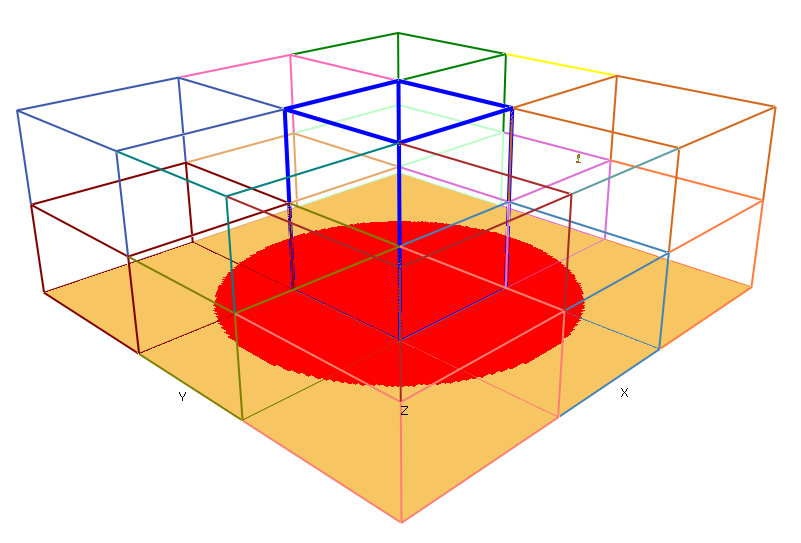
\includegraphics[width=0.83\textwidth]{images/ModellmitgrBrandherd.png}
    \caption{Mesheinteilung bei Modell mit 3 m Raumhöhe und max. spez. Wärmefreisetzungsrate}
    \label{fig:MesheinteilungmitgrBrandherd}
\end{figure}
Die rote Fläche stellt die gesamte Brandfläche bei 300~s dar. Es ist zu erkennen, dass der Brand ab einem gewissen Zeitpunkt die Grenzen des inneren Mesh überschreiten und gegen Ende der Simulationszeit in alle unteren Mesh vorgedrungen sein wird. Laut dem FDS User Guide sollte vermieden werden, dass die Brandfläche verschiedene Mesh berührt \cite[S. 40]{FDSUser}. Dies muss bei der Auswertung der Ergebnisse berücksichtigt werden.

Um den Einfluss dieses Brandherdes mit einer geringeren maximalen spezifischen Wärmefreisetzungsrate zu untersuchen, wird der zeitliche Verlauf der Sprinklerelementtemperatur bei verschiedenen Raumhöhen mit den Daten aus Kap. \ref{sec:VergleichSimulationundBerechnung} in Abb. \ref{fig:AltBrandherdVerlauf} verglichen. 
\begin{figure}
    \centering
    \includegraphics[width=\textwidth]{images/AltBrandherdVerlauf.pdf}
    \caption{Vergleich der Sprinklerelementtemperatur zwischen Simulationen mit $\Dot{q}_{max}=500$~kW/m² (Sim.*) und $\Dot{q}_{max}=5386$~kW/m² (Sim.) bei verschiedenen Raumhöhen.}
    \label{fig:AltBrandherdVerlauf}
\end{figure}
Während die beiden Verläufe mit $H=3$~m bis ca. 170~s so gut wie keine Abweichungen aufweisen, besteht ab diesem Zeitpunkt eine deutliche Divergenz. Die Elementtemperatur der Simulation mit $\Dot{q}_{max}=500$~kW/m² weicht stark vom bis dahin exponentiellen Verlauf ab und folgt bis zum Ende der Simulation einem schwächeren, annähernd linearen Verlauf. 
Allerdings beträgt die Sprinklerelementtemperatur zum Zeitpunkt von 170~s bei beiden Brandherden schon über 125~°C und die Abweichung hat nur noch einen Einfluss auf die Sprinklerköpfe mit einer Nennöffnungstemperatur von 141~°C \bzw 182~°C. 


Bei den Verläufen mit 6~m und 8~m ist keine große Abweichung erkennbar. Dies wird auch ersichtlich in Tab. \ref{tab:altBrandherdErgebnisse}, welche die Ergebnisse der verschiedenen Auslösezeiten zusätzlich noch mit den Berechnungen nach SFPE-Handbook und VDI-Tabelle vergleicht.
\begin{table}\centering
\caption{Vergleich der Sprinklerauslösezeiten (in s) zwischen Simulationen mit $\Dot{q}_{max}=500$~kW/m² (Sim.*), $\Dot{q}_{max}=5386$~kW/m² (Sim.), Berechnungen nach SFPE-Handbuch und VDI-Tabellenwerten für verschiedene Nennöffnungstemperaturen (Trd; in °C)  und Raumhöhen ($\alpha=0{,}047$~kW/s², RTI $=50$~(m/s)$^{0,5}$).}
\label{tab:altBrandherdErgebnisse}
\begin{tabu} to 0.7\textwidth{@{}X[c]X[c]X[c]X[c]X[c]X@{}} \toprule
Trd                 &       & H = 3 m & H = 6 m          & H = 8 m          \\
    \midrule
\multirow{4}{*}{57} & Sim.* & 105     & 142              & 163              \\
                    & Sim.  & 102     & 143              & 170              \\
                    & SFPE  & 104     & 135              & 157              \\
                    & VDI   & 105     & 140              & 160              \\
                    \midrule
\multirow{4}{*}{68} & Sim.* & 115     & 163              & 192              \\
                    & Sim.  & 116     & 165              & 194              \\
                    & SFPE  & 116     & 153              & 179              \\
                    & VDI   & 120     & 155              & 185              \\
                    \midrule
\multirow{4}{*}{79} & Sim.* & 127     & 183              & 221              \\
                    & Sim.  & 126     & 183              & 212              \\
                    & SFPE  & 126     & 169              & 200              \\
                    & VDI   & 130     & 175              & 205              \\
                    \midrule
\multirow{4}{*}{93} & Sim.* & 144     & 209              & 252              \\
                    & Sim.  & 140     & 210              & 259              \\
                    & SFPE  & 139     & 189              & 226              \\
                    & VDI   & 140     & 195              & 230              \\
                    \midrule
\multirow{4}{*}{141}& Sim.* & 188     & 289              & \textgreater 300 \\
                    & Sim.  & 189     & 271              & \textgreater 300 \\
                    & SFPE  & 178     & 252              & 306              \\
                    & VDI   & 180     & 260              & 315              \\
                    \midrule
\multirow{4}{*}{182}& Sim.* & 228     & \textgreater 300 & \textgreater 300 \\
                    & Sim.  & 191     & \textgreater 300 & \textgreater 300 \\
                    & SFPE  & 208     & 301              & 371              \\
                    & VDI   & 215     & 310              & 380              \\
    \bottomrule
\end{tabu}
\end{table}
Differenzen größer 10~s zwischen den beiden Simulationen sind erst ab Nennauslösetemperaturen größer 141~°C zu erkennen. Dabei liegen Auslösezeiten der Simulationen mit $\Dot{q}_{max}=500$~kW/m² aufgrund des flacheren Anstiegs der Sprinklerelementtemperatur grundsätzlich höher.

Abb.~\ref{fig:GastempAltBrandherd} und Abb.~\ref{fig:GasgeschwAltBrandherd} zeigen hierfür den Unterschied in der Gastemperatur und -geschwindigkeit am Sprinklerkopf bei einer Raumhöhe von 3~m auf.
\begin{figure}
    \centering
    \includegraphics[width=0.83\textwidth]{images/AltBrandherdGasTemp.pdf}
    \caption{Verlauf der Rauchgastemperatur am Sprinklerkopf bei verschiedenen max. spez. Wärmefreisetzungsraten mit Sim.: $\Dot{q}_{max}=5386$~kW/m² und Sim.*: $\Dot{q}_{max}=500$~kW/m².}
    \label{fig:GastempAltBrandherd}
\end{figure}
\begin{figure}
    \centering
    \includegraphics[width=0.83\textwidth]{images/AltBrandherdGasGeschw.pdf}
    \caption{Verlauf der Rauchgasgeschwindigkeit am Sprinklerkopf bei verschiedenen max. spez. Wärmefreisetzungsraten mit Sim.: $\Dot{q}_{max}=5386$~kW/m² und Sim.*: $\Dot{q}_{max}=500$~kW/m².}
    \label{fig:GasgeschwAltBrandherd}
\end{figure}
Ab ca. 170~s steigt die Gastemperatur mit $\Dot{q}_{max}=5386$~kW/m² stärker an als die Temperatur mit $\Dot{q}_{max}=500$~kW/m². Grund dafür ist die niedrigere spezifische Wärmefreisetzungsrate der Simulation mit $\Dot{q}_{max}=500$~kW/m². Da mit der im Verhältnis größeren Brandfläche auch ein größerer Plume entsteht, wird mehr Luft induziert und erwärmt. Dies führt zu einer niedrigeren Gastemperatur und somit auch zu einer niedrigeren Sprinklerelementtemperatur. Die Geschwindigkeit des Deckenstrahls erhöht sich dabei, da ein größeres Rauchvolumen an die Decke strömt. 
Ein weiterer Faktor für die Abweichung könnte auf eine Limitierung des Simulationmodells hinweisen. Da bei einer großen Brandfläche die für diese Arbeit definierte Mesheinteilung nicht ideal ist und der Brandherd ab 219~s die Meshgrenzen überschreitet, kann es zu Datenverlusten und Fehlern in der Simulation kommen.

Die Bedeutung der Brandherdgröße und maximalen spezifischen Wärmefreisetzungsrate muss in nachfolgenden Arbeiten näher betrachtet werden. Allerdings kann ausgesagt werden, dass vor allem in der Anfangsphase auch Simulationen mit einer größeren Brandherdgröße zu sehr guten Übereinstimmungen mit den Berechnungen nach SFPE-Handbook führen. 







%%%%%%%%%%%%%%%%%%%%%%%%%%%%%%%%%%%%%%%%%%%%%%%%
\FloatBarrier
\section{Visuelle Auswertung}
\label{VisuelleAuswertung}

Abb.~\ref{fig:visA} zeigt den gesamten Verlauf der Simulation mit Sprinkleraktivierung. Die Wärmefreisetzungsrate von 1~kW wird Abb.~\ref{fig:visA1} überschritten und der Brand beginnt. Der Plume des Feuers steigt auf, erreicht die Decke und der Rauch breitet sich radial an der Decke aus. In Abb.~\ref{fig:visA3} ist zu erkennen, dass der gesamte Deckenbereich mit Rauch gefüllt ist und sich eine Rauchgasschicht und raucharme Schicht etabliert hat. Bei 122,4~s hat das Sprinklerauslöseelement die Nennöffnungstemperatur von 68~°C erreicht und der Sprinklerkopf löst aus. Wasser wird rundum verteilt und verhindert ein weiteres Ausbreiten des Feuers. Die Wärmefreisetzungsrate wird begrenzt.
\begin{figure}[h]\centering
\subfigure[][]{%
\label{fig:visA1}%
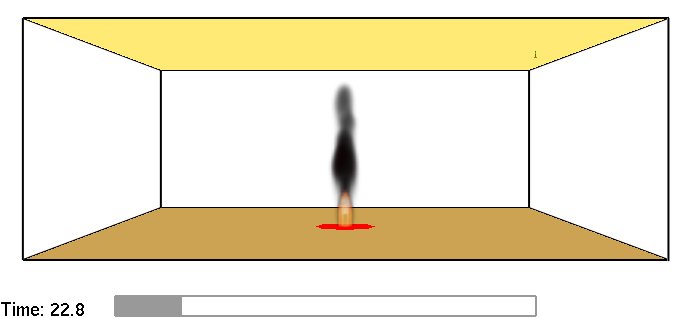
\includegraphics[width=.48\textwidth]{images/FDSBilder/VisuelleAuswertung1.png}}%
\hspace{8pt}%
\subfigure[][]{%
\label{fig:visA2}%
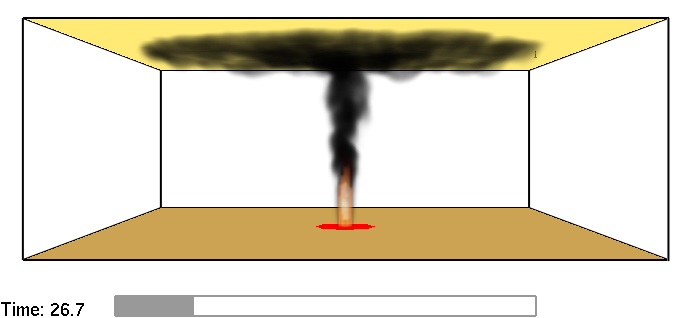
\includegraphics[width=.48\textwidth]{images/FDSBilder/VisuelleAuswertung2.png}}\\
\subfigure[][]{%
\label{fig:visA3}%
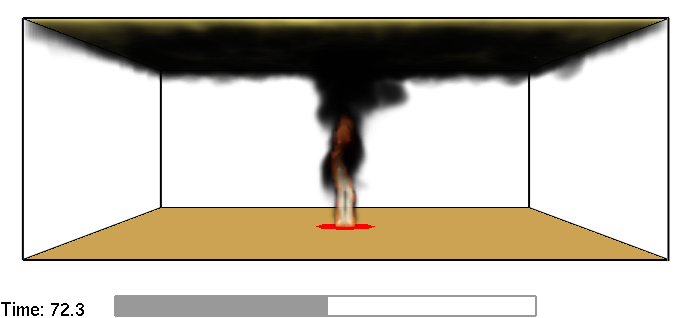
\includegraphics[width=.48\textwidth]{images/FDSBilder/VisuelleAuswertung3.png}}%
\hspace{8pt}%
\subfigure[][]{%
\label{fig:visA4}%
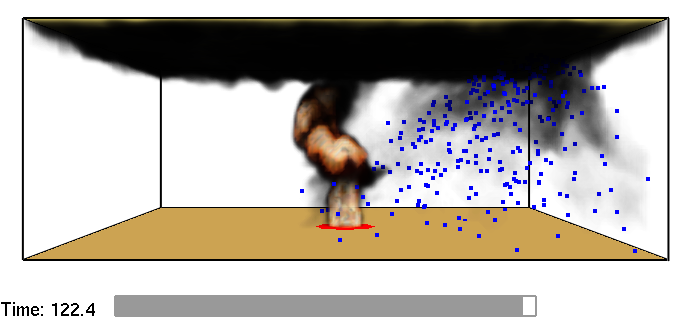
\includegraphics[width=.48\textwidth]{images/FDSBilder/VisuelleAuswertung4.png}}%
\caption{Brandverlauf mit Sprinkleraktivierung in Smokeview (H = 3~m, $\alpha=0,047$ kW/s², C = 0, Trd = 68~°C).}%
\label{fig:visA}%
\end{figure}

FDS ermöglicht es mithilfe der Plot3D Funktion, Vektoren für jede einzelne Zelle in Smokeview simulieren zu lassen. Abb.~\ref{fig:VektorenPlume} stellt den Plume und Ceiling Jet in der Vektoransicht bei 70~s dar. Es ist zu erkennen, dass der aus dem Brand entstandene Rauch mit hoher Geschwindigkeit an die Decke steigt. Kalte Umgebungsluft wird in Plume induziert und kühlt diesen ab. Eine große Verwirbelung auf der linken Seite des Plumes ist auszumachen. Auch am Ceiling Jet selbst wird Luft induziert. Das Rauchgas ist deutlich abgekühlt, wenn es den Sprinklerkopf erreicht. 
\begin{figure}
    \centering
    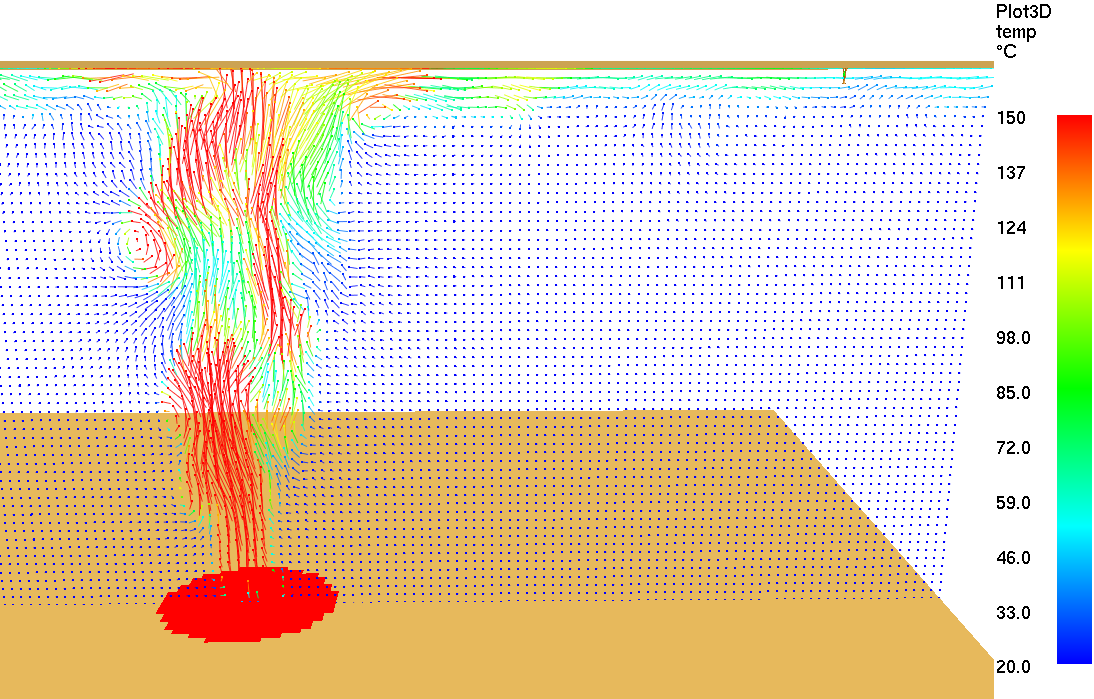
\includegraphics[width=\textwidth]{images/FDSBilder/VektorenPlume.png}
    \caption{Vektordarstellung bei Sekunde 70 (H = 3~m, $\alpha=0,047$ kW/s², C = 0, Trd = 68~°C).}
    \label{fig:VektorenPlume}
\end{figure}
Eine nähere Betrachtung des Bereiches um den Sprinklerkopf herum, zeigt zum selben Zeitpunkt, die Verwirbelungen um den Sprinklerkopf herum auf (siehe Abb.~\ref{fig:VektorenSprinkler}). Wellen heißer Luft erreichen das Auslöseelement. Dieses wird meist horizontal aus Richtung des Brandherdes angeströmt.
\begin{figure}
    \centering
    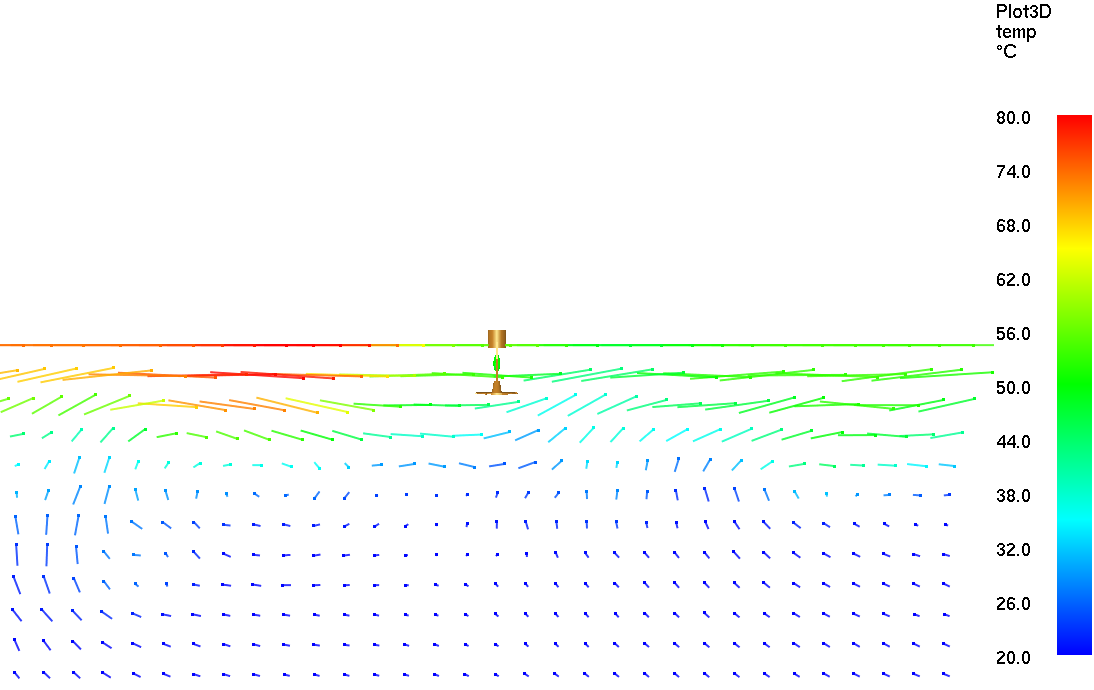
\includegraphics[width=\textwidth]{images/FDSBilder/VektorSprinklerkopf.png}
    \caption{Vektordarstellung am Sprinklerkopf bei Sekunde 70 (H = 3~m, $\alpha=0,047$ kW/s², C = 0, Trd = 68~°C).}
    \label{fig:VektorenSprinkler}
\end{figure}
\clearpage
\SuperPar
Abb.~\ref{fig:PlumeTemp} zeigt eine weitere Anwendung der Plot3D Funktion in Smokeview. Hierbei werden alle Zellenpunkte, die eine bestimmte Temperatur aufweisen, miteinander verbunden und schattiert. In diesem Fall wird die Isofläche des 62,8~°C heißen Rauchgases bei 70~s dargestellt. Man erkennt den aufsteigenden Plume und Ceiling Jet und die relativ gleichmäßige Verteilung an der Decke. Die Verwirbelung an der linken Seite des Plumes aus Abb.~\ref{fig:VektorenPlume} ist ebenfalls zu erkennen.
\begin{figure}[h]
    \centering
    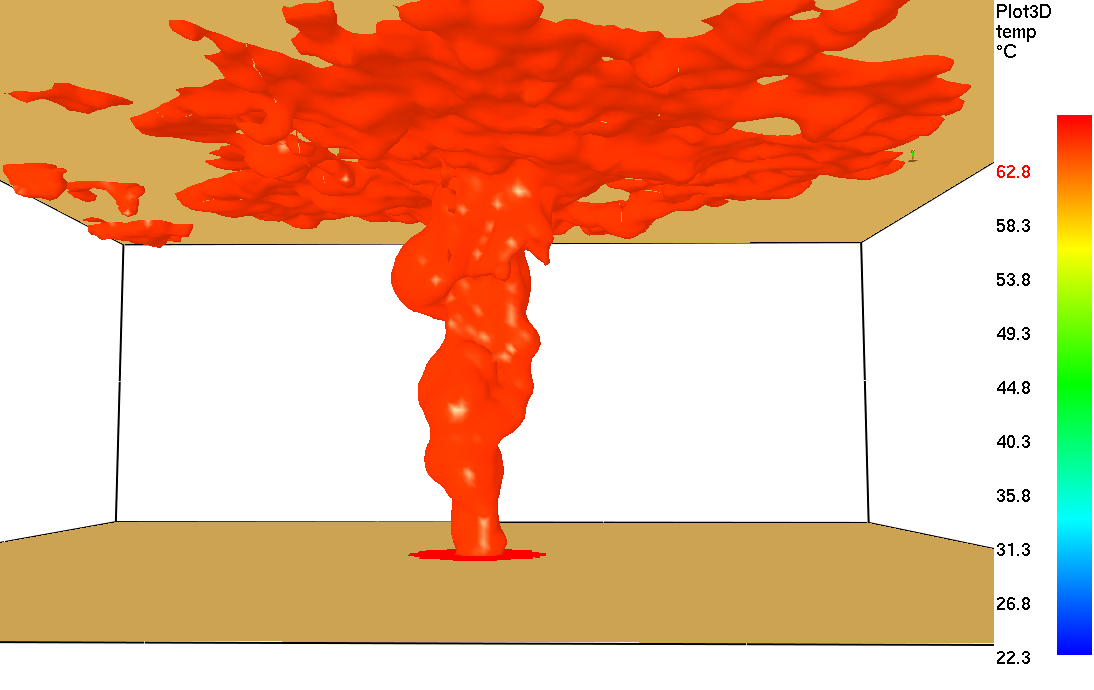
\includegraphics[width=\textwidth]{images/FDSBilder/PlumeTemp.png}
    \caption{Vektordarstellung am Sprinklerkopf bei Sekunde 70 (H = 3~m, $\alpha=0,047$ kW/s², C = 0, Trd = 68~°C).}
    \label{fig:PlumeTemp}
\end{figure}
\clearpage
\SuperPar
Zuletzt wird in Abb.~\ref{fig:PlotEcken} die Isoflächen der Luftgeschwindigkeit untersucht. Die dargestellten Flächen, besitzen eine Luftgeschwindigkeit von 0,04~m/s bei 70~s der Simulation. In der Mitte des Raumes ist die Luftgeschwindigkeit, außer ein paar kleine Ausnahmen, schneller als 0,04~m/s und in den Ecken des Raumes langsamer als dieser Wert. Es scheint, dass die Nachströmung der Luft nicht gleichmäßig aus allen Richtungen erfolgt. Da der Brandherd eine kreisförmige Fläche besitzt, müsste die Luft auch aus den Ecken strömen. Dies ist wahrscheinlich auf die mangelhafte Druckauflösung von FDS an den Raumgrenzen zurückzuführen.

\begin{figure}[h]
    \centering
    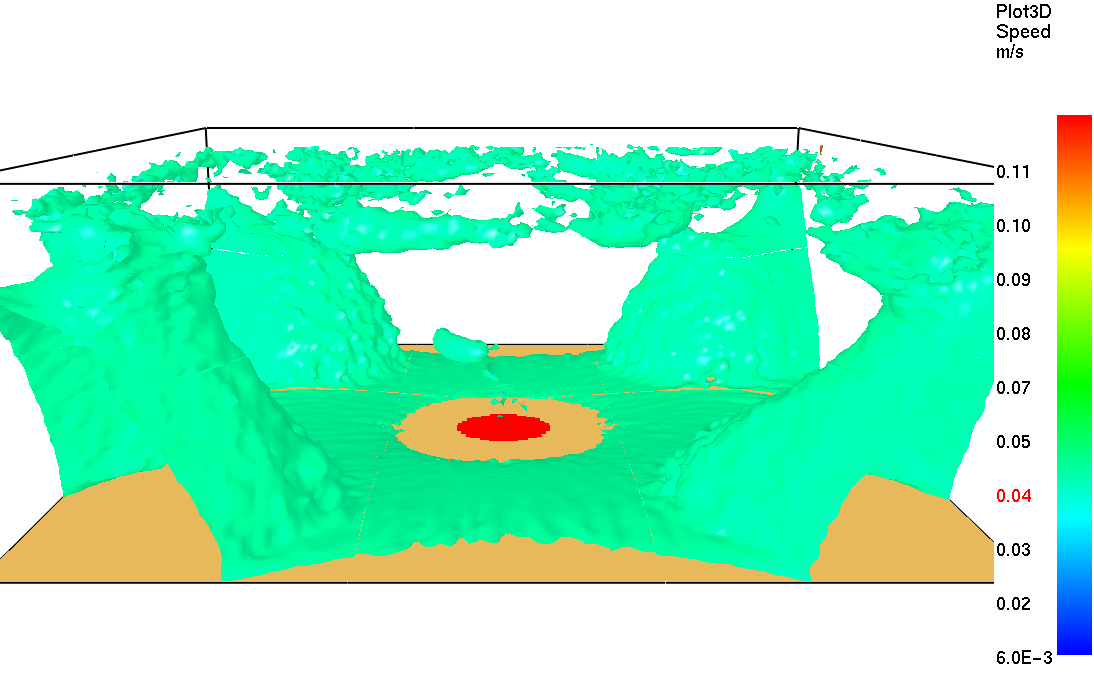
\includegraphics[width=\textwidth]{images/FDSBilder/PlotEcken.png}
    \caption{Vektordarstellung am Sprinklerkopf bei Sekunde 70 (H = 3~m, $\alpha=0,047$ kW/s², C = 0, Trd = 68~°C).}
    \label{fig:PlotEcken}
\end{figure}













\begin{comment}
\begin{figure}%
\centering
\subfigure[][]{%
\label{fig:visA1}%
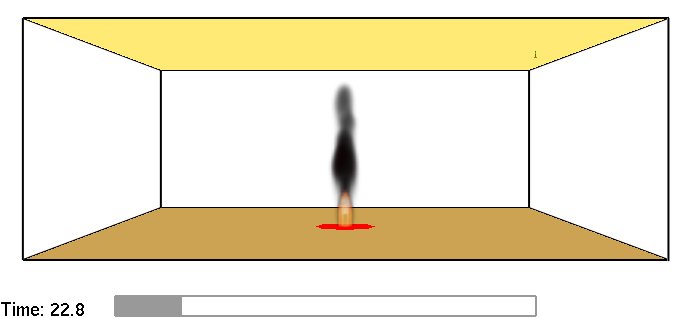
\includegraphics[width=.45\textwidth]{images/FDSBilder/VisuelleAuswertung1.png}}%
\hspace{8pt}%
\subfigure[][]{%
\label{fig:visA2}%
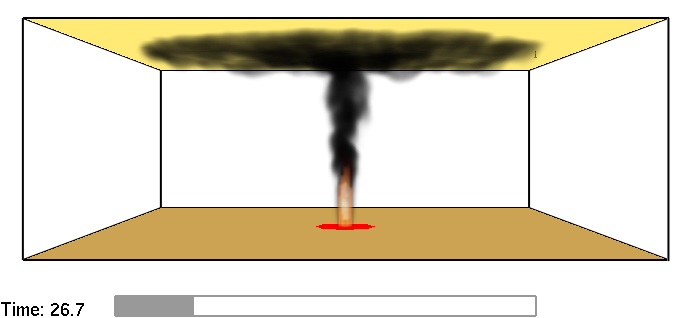
\includegraphics[width=.45\textwidth]{images/FDSBilder/VisuelleAuswertung2.png}}\\
\subfigure[][]{%
\label{fig:visA3}%
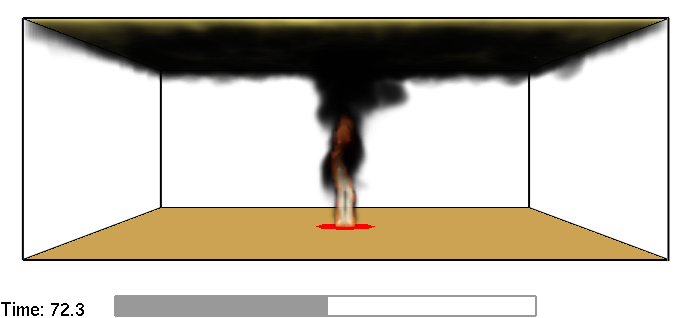
\includegraphics[width=.45\textwidth]{images/FDSBilder/VisuelleAuswertung3.png}}%
\hspace{8pt}%
\subfigure[][]{%
\label{fig:visA4}%
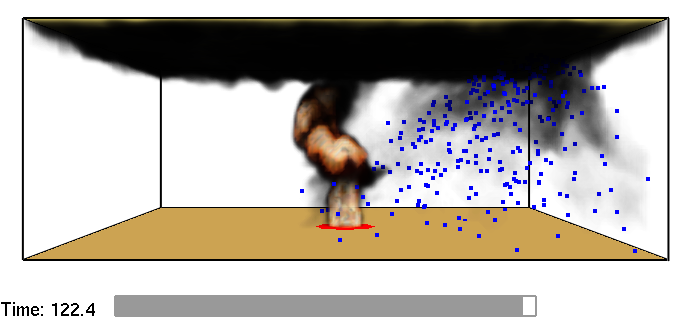
\includegraphics[width=.45\textwidth]{images/FDSBilder/VisuelleAuswertung4.png}}%
\caption{Brandverlauf mit Sprinkleraktivierung bei H = 3~m, $\alpha=0,047$ kW/s², C = 0, Trd = 68~°C.
\subref{fig:visA1} describes the first subfigure;
\subref{fig:visA2} describes the second subfigure;
\subref{fig:visA3} describes the third subfigure;
and,\subref{fig:visA4} describes the last subfigure.}%
\label{fig:visA}%
\end{figure}
\end{comment} 


%\chapter{Fazit und Ausblick}
\label{cha:Fazit}


%%%%%%%%%%%%%%%%%%%%%%%%%%%%%%%%%%%%%%%%%%%%%%%%%%%%%%%%%%%%%%%
\begin{comment}
Sprinklerauslösezeiten vorauszusagen gestaltet sich aufgrund vieler verschiedener Einflussgrößen schwierig. Zwar gibt es Berechnungsansätze, welche idealisierte Brandvorgänge abbilden können, es fehlen jedoch wichtige Variablen wie \zB die in den vorherigen Kapiteln angesprochene spezifische maximale Wärmefreisetzungsrate oder die Wärmestrahlung.
Wie in dieser Arbeit aufgezeigt wird, kann FDS mit großer Übereinstimmung zu den Berechnungen Sprinklerauslösezeiten vorhersagen. Es gilt in nachfolgenden Arbeiten zu untersuchen, wie gut FDS auch komplexere und der Realität nähere Brandszenarien abbilden kann. 
Außerdem sollten weitere Parameter, die in dieser Arbeit nicht beachtet werden, genauer untersucht werden. Was passiert, wenn sich das Auslöseelement im Windschatten des Sprinklerarms befindet? Wie wirkt sich ein Unterzug an der Decke auf die Rauchausbreitung und Auslösezeit aus?
FDS kann bei diesen Fragen Hilfestellung leisten, allerdings sind intrinsische Herausforderungen, wie \zB die Gridauflösung und -aufteilung zuerst zu bewältigen. Die Rechendauer für die simulierten Räume in dieser Arbeit betrug meist ca. 18~Stunden. Wenn Brandszenarien mit mehreren zusammenhängenden Räumen oder gar ganze Gebäude simuliert werden sollen, steigt natürlich auch die Rechendauer \bzw die Qualität der Ergebnisse nimmt mit einer geringeren Auflösung ab.

Die VDI-Richtlinie 6019-1:2006 entspricht nicht mehr dem derzeitigen wissenschaftlichen Stand, wie diese Arbeit bestätigen konnte, allerdings befindet sie sich momentan in der Erneuerung. Die in den Tabellen der VDI 6019-1 angeführten Sprinklerauslösezeiten sind zu hoch angesetzt. Simulationen, die angestellt werden um Brandschutzkonzepte zu validieren und Entrauchungsanlagen auszulegen, benötigen Informationen zum Sprinklerverhalten. Mithilfe dieser Auslösezeiten kann bestimmt werden, wann die Wärmefreisetzungsrate durch die Sprinkleranlage begrenzt wird und welche Menge an Rauch freigesetzt wird. Somit kann geschlussfolgert werden, dass zu lange Sprinklerauslösezeiten zu überdimensionierten Entrauchungsanlagen führen. Größere Kanäle und Anlagen brauchen mehr Platz und erhöhen die Kosten.
In Zukunft könnte mithilfe von FDS die Simulation des Brandherdes und der Sprinkler zusammen mit Entrauchungssimulationen durchgeführt werden, allerdings sind die oben genannten Einschränkungen von FDS zu berücksichtigen. 

Bei der Entstehung dieser Arbeit wird ein zweiter Vergleich mit den Berechnungen des SFPE-Handbooks gezogen, da diese die aktuellen Berechnungsansätze für Sprinklerauslösezeiten beinhalten. FDS liefert eine überzeugende Übereinstimmung der Sprinklerauslösezeiten zu den Berechnungen. Abweichungen betragen meist nur wenige Sekunden. Große Unregelmäßigkeiten treten meist erst auf, wenn die gebräuchlichen Nennöffnungstemperaturen der Sprinklerauslöselemente bereits überschritten wurden. Auch niedrige maximale spezifische Wärmefreisetzungsraten unterstützen die Berechnungsansätze, müssen allerdings genauer untersucht werden. Diese Arbeit zeigt auf, dass FDS in der Lage ist, Sprinklerauslösezeiten zufriedenstellend vorherzusagen.  
\end{comment}
%%%%%%%%%%%%%%%%%%%%%%%%%%%%%%%%%%%%%%%%%%%%%%%%%%%%%%%%%%%%%

Sprinklerauslösezeiten berechnen bzw. simulieren zu können, ist entscheidend für eine gewissenhafte und korrekte Entrauchungssimulation. Zu welchem Zeitpunkt die Sprinkleranlage auslöst, bestimmt, wann die Wärmefreisetzungsrate begrenzt und die Alarmierungskette in Gang gesetzt wird. Anschließend kann damit berechnet werden, welche Mengen an Rauch freigesetzt werden. Mit diesen Daten werden Brandschutzkonzepte überprüft und Entrauchungsanlagen ausgelegt. Zu klein dimensionierte Entrauchungsanlagen führen im Notfall zu einer Gefährdung von Menschenleben durch mangelnde Rauchfreihaltung der Flucht- und Rettungswege. Überdimensionierte Anlagen dagegen benötigen mehr Platz und erhöhen die Baukosten. Da die Leistung der zweiten Brandphase exponentiell ansteigt, entscheiden wenige Minuten über Wärmefreisetzungsraten im Megawattbereich.

Wie diese Arbeit aufzeigt, kann FDS mit großer Übereinstimmung zu den Berechnungen des SFPE-Handbooks Sprinklerauslösezeiten vorhersagen. Die Untersuchung des C-Faktors ergibt, dass sowohl die Literatur, als auch die angestellten Simulationen im Vergleich zu den Berechnungen einen C-Faktor von 0~(m/s)$^{0,5}$ unterstützen.
Große Unregelmäßigkeiten treten meist erst auf, wenn die gebräuchlichen Nenn\-öff\-nungs\-tem\-pe\-ra\-tur\-en der Sprinklerauslöseelemente bereits überschritten wurden. Auch niedrige maximale spezifische Wärmefreisetzungsraten unterstützen die Berechnungsansätze, müssen allerdings genauer untersucht werden. 
%Diese Arbeit zeigt auf, dass FDS in der Lage ist, Sprinklerauslösezeiten hinreichend vorherzusagen.  

Die VDI-Richtlinie 6019-1:2006 entspricht nicht mehr dem derzeitigen wissenschaftlichen Stand, wie diese Arbeit bestätigen konnte, allerdings befindet sie sich aus diesem Grund in der Überarbeitung. Die in den Tabellen der VDI 6019-1 angeführten Sprinklerauslösezeiten sind zu hoch angesetzt. Es wird sich hier auf eine wissenschaftliche Veröffentlichung berufen, die fehlerhafte Formeln beinhaltet.

Die Rechendauer für die simulierten Räume in dieser Arbeit betrug meist ca. 18~Stunden. Wenn Brandszenarien mit mehreren zusammenhängenden Räumen oder gar großvolumige Bereiche mit komplexen Geometrien simuliert werden sollen, steigt damit auch die Rechendauer \bzw die Qualität der Ergebnisse nimmt mit einer geringeren Auflösung ab.

Es gilt in nachfolgenden Arbeiten zu analysieren, wie gut FDS auch komplexere und der Realität nähere Brandszenarien abbilden kann. 
Außerdem sollten weitere Parameter, die in dieser Arbeit nicht beachtet werden, genauer untersucht werden. Was passiert, wenn sich das Auslöseelement im Windschatten des Sprinklerarms befindet? Wie wirkt sich ein Unterzug an der Decke auf die Rauchausbreitung und Auslösezeit aus?
FDS kann bei diesen Fragen Hilfestellung leisten, allerdings sind intrinsische Herausforderungen wie \zB die Gridauflösung und -aufteilung zuerst zu bewältigen. 
%%%%%%%%%%%%%%%%%%%%%%%%%%%%%%%%%%%%%%%%%%%%%%%%%%%%%%%%%%%%%

\begin{comment}
Insgesamt kann davon ausgegangen werden, dass in Zukunft immer mehr Brandschutzkonzepte mithilfe von CFD-Software validiert werden. 

 Echte Brandversuche sind sehr teuer und stellen keine wirtschaftliche Alternative dar.

zeigt aber auch die vielen möglichkeiten von fds auf

In Deutschland beträgt die maximale Auslösezeit für Sprinkler gemäß VDI 6019 Blatt 1{\cite{VDI6019B1}} 900 Sekunden. 
Fazit:

langsam ansteigende Elementtemperatur führt zu ungenaueren ergebnissen mit fds 



brandherd am boden oft unrealistisch. bei räumen mit hoher Deckenhöhe befindet sich die Brandlast wahrscheinlich auch weiter unter der Decke.




Sprinkler dürfen auch nicht zu früh öffnen 

SFPE Handbuch geht nicht auf die max. spez. Wärmefreisetzungsrate


was in zukunft beachtet werden muss:
\begin{itemize}
    \item HRR Kurve ist treppenförmig. entspricht nicht genau der t2 kurve
    \item unterschiedliche gasarten müssten untersucht werden
    \item Modell muss weiter verbessert werden
\end{itemize}

\end{comment}


%%%----------------------------------------------------------
\appendix                                            % Anhang 
%%%----------------------------------------------------------
\chapter{Ergänzende Inhalte} % \chapter{Inhalt der CD-ROM/DVD}
\label{app:materials}


Auflistung der ergänzenden Materialien zu dieser Arbeit, die zur digitalen Archivierung an der 
Hochschule eingereicht wurden (als ZIP-Datei).

% Nur als Beispiel, die Struktur sollte man an die eigenen Bedürfnisse anpassen!

\section{PDF-Dateien}
\begin{FileList}{/}
\fitem{thesis.pdf} Finale Master-/Bachelorarbeit (Gesamtdokument)
\end{FileList}

\section{Mediendaten}
\begin{FileList}{/media}
\fitem{*.ai, *.pdf} Adobe Illustrator-Dateien
\fitem{*.jpg, *.png} Rasterbilder
\fitem{*.mp3} Audio-Dateien
\fitem{*.mp4} Video-Dateien
\end{FileList}


\section{Online-Quellen (PDF-Kopien)}
\begin{FileList}{/online-sources}
\fitem{Reliquienschrein-Wikipedia.pdf} {\backtrackerfalse\parencite{WikiReliquienschrein2023}}
\end{FileList}
	% Inhalt der CD-ROM/DVD
\chapter{FDS Input-Dateien}
\label{ch:InputDateien}

\section{Brandintensitätskoeffizient}
\subsection*{Brandintensitätskoeffizient gleich 0,012~kW/s²}
\begin{lstlisting}[emptylines=0,basicstyle=\tiny]
&HEAD CHID='OffenerRaum', TITLE='0,012 bis 400s' /

&MESH ID='mesh1', COLOR='MAROON', IJK=56,56,30, XB=1.,3.8,6.2,9.,0.,1.5, MPI_PROCESS=0 /
&MESH ID='mesh2', COLOR='MELON',IJK=48,56,30, XB=3.8,6.2,6.2,9.,0.,1.5, MPI_PROCESS=1 /
&MESH ID='mesh3', COLOR='MINT', IJK=56,56,30, XB=6.2,9.,6.2,9.,0.,1.5, MPI_PROCESS=2 /
&MESH ID='mesh4', COLOR='OLIVE', IJK=56,48,30, XB=1.,3.8,3.8,6.2,0.,1.5, MPI_PROCESS=3 /
&MESH ID='mesh5', COLOR='ORCHID', IJK=56,48,30, XB=6.2,9.,3.8,6.2,0.,1.5, MPI_PROCESS=4 /
&MESH ID='mesh6', COLOR='SALMON', IJK=56,56,30, XB=1.,3.8,1.,3.8,0.,1.5, MPI_PROCESS=5 /
&MESH ID='mesh7', COLOR='STEEL BLUE', IJK=48,56,30, XB=3.8,6.2,1.,3.8,0.,1.5, MPI_PROCESS=6 /
&MESH ID='mesh8', COLOR='FLESH', IJK=56,56,30, XB=6.2,9.,1.,3.8,0.,1.5, MPI_PROCESS=7 /
&MESH ID='mesh9', COLOR='BLUE', IJK=48,48,60, XB=3.8,6.2,3.8,6.2,0.,3., MPI_PROCESS=8 /
&MESH ID='mesh10', COLOR='CHOCOLATE', IJK=56,56,30, XB=6.2,9.,1.,3.8,1.5,3., MPI_PROCESS=9 /
&MESH ID='mesh11', COLOR='COBALT', IJK=56,56,30, XB=1.,3.8,6.2,9.,1.5,3., MPI_PROCESS=10 /
&MESH ID='mesh12', COLOR='HOT PINK',IJK=48,56,30, XB=3.8,6.2,6.2,9.,1.5,3., MPI_PROCESS=11 /
&MESH ID='mesh13', COLOR='KELLY GREEN', IJK=56,56,30, XB=6.2,9.,6.2,9.,1.5,3., MPI_PROCESS=12 /
&MESH ID='mesh14', COLOR='TEAL', IJK=56,48,30, XB=1.,3.8,3.8,6.2,1.5,3., MPI_PROCESS=13 /
&MESH ID='mesh15', COLOR='YELLOW', IJK=56,48,30, XB=6.2,9.,3.8,6.2,1.5,3., MPI_PROCESS=14 /
&MESH ID='mesh16', COLOR='BROWN', IJK=56,56,30, XB=1.,3.8,1.,3.8,1.5,3., MPI_PROCESS=15 /
&MESH ID='mesh17', COLOR='CADET BLUE', IJK=48,56,30, XB=3.8,6.2,1.,3.8,1.5,3., MPI_PROCESS=16 /

&MISC VERBOSE=.TRUE./
&RADI RADIATION=.FALSE. /

&TIME T_END=400. /


&REAC FUEL = 'METHANE', SOOT_YIELD = 0.2, CO_YIELD = 0.10, RADIATIVE_FRACTION=0.3 /

&SURF ID='BURNER', HRRPUA=1086.5, TAU_MF=0.01 /
&VENT XB=4.25,5.75,4.25,5.75,0.00,0.00, XYZ=5.0,5.0,0.00, RADIUS=0.75, SPREAD_RATE=0.001875, COLOR='RED', SURF_ID='BURNER' /


&VENT MB='XMIN', SURF_ID='OPEN' /  
&VENT MB='XMAX', SURF_ID='OPEN' /  
&VENT MB='YMIN', SURF_ID='OPEN' /  
&VENT MB='YMAX', SURF_ID='OPEN' / 
 
&SPEC ID='WATER VAPOR' /
&PART ID='my droplets', DIAMETER=1000., SPEC_ID='WATER VAPOR' /
&PROP ID='K-11', QUANTITY='SPRINKLER LINK TEMPERATURE', RTI=50., C_FACTOR=0.0, ACTIVATION_TEMPERATURE=680., PART_ID='my droplets', FLOW_RATE=300.0, PARTICLE_VELOCITY=10., SMOKEVIEW_ID='sprinkler_pendent' /
&DEVC ID='Spr-1', XYZ=5.0,1.75,2.97, PROP_ID='K-11' /

&DEVC XYZ=5.0,1.75,2.97, QUANTITY='TEMPERATURE', ID='T-1'/
&DEVC XYZ=5.0,1.75,2.97, QUANTITY='VELOCITY', ID='U-1'/


&CTRL ID='kill', FUNCTION_TYPE='KILL', INPUT_ID='delay' /
&CTRL ID='delay', FUNCTION_TYPE='TIME_DELAY', INPUT_ID='Spr-1', DELAY=5. /

&DUMP DT_HRR=1.0, DT_BNDF=1.0, DT_DEVC=1.0 /

&SLCF PBX=5., QUANTITY='TEMPERATURE' /
&SLCF PBZ=2.95, QUANTITY='TEMPERATURE' /
&SLCF PBX=5., QUANTITY='VELOCITY' /



&TAIL /


\end{lstlisting}

\subsection*{Brandintensitätskoeffizient gleich 0,188~kW/s²}
\begin{lstlisting}[emptylines=0,basicstyle=\tiny]
&HEAD CHID='OffenerRaum', TITLE='0,188 bis 300s' /

&MESH ID='mesh1', COLOR='MAROON', IJK=56,56,30, XB=1.,3.8,6.2,9.,0.,1.5, MPI_PROCESS=0 /
&MESH ID='mesh2', COLOR='MELON',IJK=48,56,30, XB=3.8,6.2,6.2,9.,0.,1.5, MPI_PROCESS=1 /
&MESH ID='mesh3', COLOR='MINT', IJK=56,56,30, XB=6.2,9.,6.2,9.,0.,1.5, MPI_PROCESS=2 /
&MESH ID='mesh4', COLOR='OLIVE', IJK=56,48,30, XB=1.,3.8,3.8,6.2,0.,1.5, MPI_PROCESS=3 /
&MESH ID='mesh5', COLOR='ORCHID', IJK=56,48,30, XB=6.2,9.,3.8,6.2,0.,1.5, MPI_PROCESS=4 /
&MESH ID='mesh6', COLOR='SALMON', IJK=56,56,30, XB=1.,3.8,1.,3.8,0.,1.5, MPI_PROCESS=5 /
&MESH ID='mesh7', COLOR='STEEL BLUE', IJK=48,56,30, XB=3.8,6.2,1.,3.8,0.,1.5, MPI_PROCESS=6 /
&MESH ID='mesh8', COLOR='FLESH', IJK=56,56,30, XB=6.2,9.,1.,3.8,0.,1.5, MPI_PROCESS=7 /
&MESH ID='mesh9', COLOR='BLUE', IJK=48,48,60, XB=3.8,6.2,3.8,6.2,0.,3., MPI_PROCESS=8 /
&MESH ID='mesh10', COLOR='CHOCOLATE', IJK=56,56,30, XB=6.2,9.,1.,3.8,1.5,3., MPI_PROCESS=9 /
&MESH ID='mesh11', COLOR='COBALT', IJK=56,56,30, XB=1.,3.8,6.2,9.,1.5,3., MPI_PROCESS=10 /
&MESH ID='mesh12', COLOR='HOT PINK',IJK=48,56,30, XB=3.8,6.2,6.2,9.,1.5,3., MPI_PROCESS=11 /
&MESH ID='mesh13', COLOR='KELLY GREEN', IJK=56,56,30, XB=6.2,9.,6.2,9.,1.5,3., MPI_PROCESS=12 /
&MESH ID='mesh14', COLOR='TEAL', IJK=56,48,30, XB=1.,3.8,3.8,6.2,1.5,3., MPI_PROCESS=13 /
&MESH ID='mesh15', COLOR='YELLOW', IJK=56,48,30, XB=6.2,9.,3.8,6.2,1.5,3., MPI_PROCESS=14 /
&MESH ID='mesh16', COLOR='BROWN', IJK=56,56,30, XB=1.,3.8,1.,3.8,1.5,3., MPI_PROCESS=15 /
&MESH ID='mesh17', COLOR='CADET BLUE', IJK=48,56,30, XB=3.8,6.2,1.,3.8,1.5,3., MPI_PROCESS=16 /
&MISC VERBOSE=.TRUE./
&RADI RADIATION=.FALSE. /

&TIME T_END=300. /


&REAC FUEL = 'METHANE', SOOT_YIELD = 0.2, CO_YIELD = 0.10, RADIATIVE_FRACTION=0.3 /

&SURF ID='BURNER', HRRPUA=21543., TAU_MF=0.01 /
&VENT XB=4.5,5.5,4.5,5.5,0.00,0.00, XYZ=5.0,5.0,0.00, RADIUS=0.5, SPREAD_RATE=0.001666, COLOR='RED', SURF_ID='BURNER' /


&VENT MB='XMIN', SURF_ID='OPEN' /  
&VENT MB='XMAX', SURF_ID='OPEN' /  
&VENT MB='YMIN', SURF_ID='OPEN' /  
&VENT MB='YMAX', SURF_ID='OPEN' / 
 
&SPEC ID='WATER VAPOR' /
&PART ID='my droplets', DIAMETER=1000., SPEC_ID='WATER VAPOR' /
&PROP ID='K-11', QUANTITY='SPRINKLER LINK TEMPERATURE', RTI=50., C_FACTOR=0.0, ACTIVATION_TEMPERATURE=6800., PART_ID='my droplets', FLOW_RATE=300.0, PARTICLE_VELOCITY=10., SMOKEVIEW_ID='sprinkler_pendent' /
&DEVC ID='Spr-1', XYZ=5.0,1.75,2.97, PROP_ID='K-11' /

&DEVC XYZ=5.0,1.75,2.97, QUANTITY='TEMPERATURE', ID='T-1'/
&DEVC XYZ=5.0,1.75,2.97, QUANTITY='VELOCITY', ID='U-1'/


&CTRL ID='kill', FUNCTION_TYPE='KILL', INPUT_ID='delay' /
&CTRL ID='delay', FUNCTION_TYPE='TIME_DELAY', INPUT_ID='Spr-1', DELAY=5. /


&DUMP DT_HRR=1.0, DT_BNDF=1.0, DT_DEVC=1.0 /

&SLCF PBX=5., QUANTITY='TEMPERATURE' /
&SLCF PBZ=2.95, QUANTITY='TEMPERATURE' /
&SLCF PBX=5., QUANTITY='VELOCITY' /



&TAIL /


\end{lstlisting}
%%%%%%%%%%%%%%%%%%%%%%%%%%%%%%%%%%%%%%%%%%%%%%%%%%%%%%%%%%%%%%%%%
\section{Brandherd mit 500 kW/m² max. spez. Wärmeleistung}
\subsection*{Raumhöhe gleich 3 m}
\begin{lstlisting}[emptylines=0,basicstyle=\tiny]
&HEAD CHID='OffenerRaum', TITLE='H=3m, a=0,047, C=0 mit alt Brandherd' /

&MESH ID='mesh1', COLOR='MAROON', IJK=56,56,30, XB=1.,3.8,6.2,9.,0.,1.5, MPI_PROCESS=0 /
&MESH ID='mesh2', COLOR='MELON',IJK=48,56,30, XB=3.8,6.2,6.2,9.,0.,1.5, MPI_PROCESS=1 /
&MESH ID='mesh3', COLOR='MINT', IJK=56,56,30, XB=6.2,9.,6.2,9.,0.,1.5, MPI_PROCESS=2 /
&MESH ID='mesh4', COLOR='OLIVE', IJK=56,48,30, XB=1.,3.8,3.8,6.2,0.,1.5, MPI_PROCESS=3 /
&MESH ID='mesh5', COLOR='ORCHID', IJK=56,48,30, XB=6.2,9.,3.8,6.2,0.,1.5, MPI_PROCESS=4 /
&MESH ID='mesh6', COLOR='SALMON', IJK=56,56,30, XB=1.,3.8,1.,3.8,0.,1.5, MPI_PROCESS=5 /
&MESH ID='mesh7', COLOR='STEEL BLUE', IJK=48,56,30, XB=3.8,6.2,1.,3.8,0.,1.5, MPI_PROCESS=6 /
&MESH ID='mesh8', COLOR='FLESH', IJK=56,56,30, XB=6.2,9.,1.,3.8,0.,1.5, MPI_PROCESS=7 /
&MESH ID='mesh9', COLOR='BLUE', IJK=48,48,60, XB=3.8,6.2,3.8,6.2,0.,3., MPI_PROCESS=8 /
&MESH ID='mesh10', COLOR='CHOCOLATE', IJK=56,56,30, XB=6.2,9.,1.,3.8,1.5,3., MPI_PROCESS=9 /
&MESH ID='mesh11', COLOR='COBALT', IJK=56,56,30, XB=1.,3.8,6.2,9.,1.5,3., MPI_PROCESS=10 /
&MESH ID='mesh12', COLOR='HOT PINK',IJK=48,56,30, XB=3.8,6.2,6.2,9.,1.5,3., MPI_PROCESS=11 /
&MESH ID='mesh13', COLOR='KELLY GREEN', IJK=56,56,30, XB=6.2,9.,6.2,9.,1.5,3., MPI_PROCESS=12 /
&MESH ID='mesh14', COLOR='TEAL', IJK=56,48,30, XB=1.,3.8,3.8,6.2,1.5,3., MPI_PROCESS=13 /
&MESH ID='mesh15', COLOR='YELLOW', IJK=56,48,30, XB=6.2,9.,3.8,6.2,1.5,3., MPI_PROCESS=14 /
&MESH ID='mesh16', COLOR='BROWN', IJK=56,56,30, XB=1.,3.8,1.,3.8,1.5,3., MPI_PROCESS=15 /
&MESH ID='mesh17', COLOR='CADET BLUE', IJK=48,56,30, XB=3.8,6.2,1.,3.8,1.5,3., MPI_PROCESS=16 /

&MISC VERBOSE=.TRUE./
&RADI RADIATION=.FALSE. /

&TIME T_END=300. /

&REAC FUEL = 'METHANE', SOOT_YIELD = 0.2, CO_YIELD = 0.10, RADIATIVE_FRACTION=0.3 /

&SURF ID='BURNER', HRRPUA=500., TAU_MF=0.01 /
&VENT XB=3.359,6.641,3.359,6.641,0.0,0.0, XYZ=5.0,5.0,0.0, RADIUS=1.641, SPREAD_RATE=0.00547, COLOR='RED', SURF_ID='BURNER' /


&VENT MB='XMIN', SURF_ID='OPEN' /  
&VENT MB='XMAX', SURF_ID='OPEN' /  
&VENT MB='YMIN', SURF_ID='OPEN' /  
&VENT MB='YMAX', SURF_ID='OPEN' / 
 
&SPEC ID='WATER VAPOR' /
&PART ID='my droplets', DIAMETER=1000., SPEC_ID='WATER VAPOR' /
&PROP ID='K-11', QUANTITY='SPRINKLER LINK TEMPERATURE', RTI=50., C_FACTOR=0.0, ACTIVATION_TEMPERATURE=6800., PART_ID='my droplets', FLOW_RATE=300.0, PARTICLE_VELOCITY=10., SMOKEVIEW_ID='sprinkler_pendent' /
&DEVC ID='Spr-1', XYZ=5.0,1.75,2.97, PROP_ID='K-11' /

&DEVC XYZ=5.0,1.75,2.97, QUANTITY='TEMPERATURE', ID='T-1'/
&DEVC XYZ=5.0,1.75,2.97, QUANTITY='VELOCITY', ID='U-1'/


&CTRL ID='kill', FUNCTION_TYPE='KILL', INPUT_ID='trigger' /
&CTRL ID='trigger', FUNCTION_TYPE='ALL', INPUT_ID='sprinklerActivated', 'delay' /
&CTRL ID='delay', FUNCTION_TYPE='TIME_DELAY', INPUT_ID='sprinklerActivated', DELAY=5. /
&CTRL ID='sprinklerActivated', FUNCTION_TYPE='AT_LEAST', N=1, INPUT_ID='Spr-1' /
&CTRL ID='Spr-1 Activated', FUNCTION_TYPE='AT_LEAST', N=1, INPUT_ID='Spr-1' /


&DUMP DT_HRR=1.0, DT_BNDF=1.0, DT_DEVC=1.0 /

&SLCF PBX=5., QUANTITY='TEMPERATURE' /
&SLCF PBZ=2.95, QUANTITY='TEMPERATURE' /
&SLCF PBX=5., QUANTITY='VELOCITY' /


&MISC RESTART=.FALSE.

&TAIL /
\end{lstlisting}

\subsection*{Raumhöhe gleich 6 m}
\begin{lstlisting}[emptylines=0,basicstyle=\tiny]
&HEAD CHID='OffenerRaum', TITLE='H=6 mit alt. Brandherd' /

&MESH ID='mesh1', COLOR='MAROON', IJK=28,28,30, XB=1.,3.8,6.2,9.,0.,3., MPI_PROCESS=0 /
&MESH ID='mesh2', COLOR='MELON',IJK=24,28,30, XB=3.8,6.2,6.2,9.,0.,3., MPI_PROCESS=1 /
&MESH ID='mesh3', COLOR='MINT', IJK=28,28,30, XB=6.2,9.,6.2,9.,0.,3., MPI_PROCESS=2 /
&MESH ID='mesh4', COLOR='OLIVE', IJK=28,24,30, XB=1.,3.8,3.8,6.2,0.,3., MPI_PROCESS=3 /
&MESH ID='mesh5', COLOR='ORCHID', IJK=28,24,30, XB=6.2,9.,3.8,6.2,0.,3., MPI_PROCESS=4 /
&MESH ID='mesh6', COLOR='SALMON', IJK=28,28,30, XB=1.,3.8,1.,3.8,0.,3., MPI_PROCESS=5 /
&MESH ID='mesh7', COLOR='STEEL BLUE', IJK=24,28,30, XB=3.8,6.2,1.,3.8,0.,3., MPI_PROCESS=6 /
&MESH ID='mesh8', COLOR='FLESH', IJK=28,28,30, XB=6.2,9.,1.,3.8,0.,3., MPI_PROCESS=7 /
&MESH ID='mesh9', COLOR='CYAN', IJK=24,24,45, XB=3.8,6.2,3.8,6.2,0.,4.5, MPI_PROCESS=8 /
&MESH ID='mesh10', COLOR='BLUE', IJK=24,24,15, XB=3.8,6.2,3.8,6.2,4.5,6., MPI_PROCESS=9 /
&MESH ID='mesh11', COLOR='CHOCOLATE', IJK=28,28,30, XB=1.,3.8,6.2,9.,3.,6., MPI_PROCESS=10 /
&MESH ID='mesh12', COLOR='COBALT',IJK=24,28,30, XB=3.8,6.2,6.2,9.,3.,6., MPI_PROCESS=11 /
&MESH ID='mesh13', COLOR='HOT PINK', IJK=28,28,30, XB=6.2,9.,6.2,9.,3.,6., MPI_PROCESS=12 /
&MESH ID='mesh14', COLOR='KELLY GREEN', IJK=28,24,30, XB=1.,3.8,3.8,6.2,3.,6., MPI_PROCESS=13 /
&MESH ID='mesh15', COLOR='TEAL', IJK=28,24,30, XB=6.2,9.,3.8,6.2,3.,6., MPI_PROCESS=14 /
&MESH ID='mesh16', COLOR='YELLOW', IJK=28,28,30, XB=1.,3.8,1.,3.8,3.,6., MPI_PROCESS=15 /
&MESH ID='mesh17', COLOR='BROWN', IJK=24,28,30, XB=3.8,6.2,1.,3.8,3.,6., MPI_PROCESS=16 /
&MESH ID='mesh18', COLOR='CADET BLUE', IJK=28,28,30, XB=6.2,9.,1.,3.8,3.,6., MPI_PROCESS=17 /

&MISC VERBOSE=.TRUE./
&RADI RADIATION=.FALSE. /

&TIME T_END=300. /

&DUMP DT_RESTART=5. /


&REAC FUEL = 'METHANE', SOOT_YIELD = 0.2, CO_YIELD = 0.10, RADIATIVE_FRACTION=0.3 /

&SURF ID='BURNER', HRRPUA=500., TAU_MF=0.01 /
&VENT XB=3.359,6.641,3.359,6.641,0.0,0.0, XYZ=5.0,5.0,0.0, RADIUS=1.641, SPREAD_RATE=0.00547, COLOR='RED', SURF_ID='BURNER' /


&VENT MB='XMIN', SURF_ID='OPEN' /  
&VENT MB='XMAX', SURF_ID='OPEN' /  
&VENT MB='YMIN', SURF_ID='OPEN' /  
&VENT MB='YMAX', SURF_ID='OPEN' / 

 
&SPEC ID='WATER VAPOR' /
&PART ID='my droplets', DIAMETER=1000., SPEC_ID='WATER VAPOR' /
&PROP ID='K-11', QUANTITY='SPRINKLER LINK TEMPERATURE', RTI=50., C_FACTOR=0.0, ACTIVATION_TEMPERATURE=6800., PART_ID='my droplets', FLOW_RATE=300.0, PARTICLE_VELOCITY=10., SMOKEVIEW_ID='sprinkler_pendent' /
&DEVC ID='Spr-1', XYZ=5.0,1.75,5.97, PROP_ID='K-11' /

&DEVC XYZ=5.0,1.75,5.97, QUANTITY='TEMPERATURE', ID='T-1'/
&DEVC XYZ=5.0,1.75,5.97, QUANTITY='VELOCITY', ID='U-1'/


&CTRL ID='kill', FUNCTION_TYPE='KILL', INPUT_ID='delay' /
&CTRL ID='delay', FUNCTION_TYPE='TIME_DELAY', INPUT_ID='Spr-1', DELAY=5. /




&DUMP DT_HRR=1.0, DT_BNDF=1.0, DT_DEVC=1.0 /

&SLCF PBX=5., QUANTITY='TEMPERATURE' /
&SLCF PBZ=2.95, QUANTITY='TEMPERATURE' /
&SLCF PBX=5., QUANTITY='VELOCITY' /


&MISC RESTART=.FALSE.

&TAIL /
\end{lstlisting}

\subsection*{Raumhöhe gleich 8 m}
\begin{lstlisting}[emptylines=0,basicstyle=\tiny]
&HEAD CHID='OffenerRaum', TITLE='H=8 mit alt. Brandherd' /

&MESH ID='mesh1', COLOR='MAROON', IJK=28,28,40, XB=1.,3.8,6.2,9.,0.,4., MPI_PROCESS=0 /
&MESH ID='mesh2', COLOR='MELON',IJK=24,28,40, XB=3.8,6.2,6.2,9.,0.,4., MPI_PROCESS=1 /
&MESH ID='mesh3', COLOR='MINT', IJK=28,28,40, XB=6.2,9.,6.2,9.,0.,4., MPI_PROCESS=2 /
&MESH ID='mesh4', COLOR='OLIVE', IJK=28,24,40, XB=1.,3.8,3.8,6.2,0.,4., MPI_PROCESS=3 /
&MESH ID='mesh5', COLOR='ORCHID', IJK=28,24,40, XB=6.2,9.,3.8,6.2,0.,4., MPI_PROCESS=4 /
&MESH ID='mesh6', COLOR='SALMON', IJK=28,28,40, XB=1.,3.8,1.,3.8,0.,4., MPI_PROCESS=5 /
&MESH ID='mesh7', COLOR='STEEL BLUE', IJK=24,28,40, XB=3.8,6.2,1.,3.8,0.,4., MPI_PROCESS=6 /
&MESH ID='mesh8', COLOR='FLESH', IJK=28,28,40, XB=6.2,9.,1.,3.8,0.,4., MPI_PROCESS=7 /
&MESH ID='mesh9', COLOR='CYAN', IJK=24,24,45, XB=3.8,6.2,3.8,6.2,0.,4.5, MPI_PROCESS=8 /
&MESH ID='mesh10', COLOR='BLUE', IJK=24,24,35, XB=3.8,6.2,3.8,6.2,4.5,8., MPI_PROCESS=9 /
&MESH ID='mesh11', COLOR='CHOCOLATE', IJK=28,28,40, XB=1.,3.8,6.2,9.,4.,8., MPI_PROCESS=10 /
&MESH ID='mesh12', COLOR='COBALT',IJK=24,28,40, XB=3.8,6.2,6.2,9.,4.,8., MPI_PROCESS=11 /
&MESH ID='mesh13', COLOR='HOT PINK', IJK=28,28,40, XB=6.2,9.,6.2,9.,4.,8., MPI_PROCESS=12 /
&MESH ID='mesh14', COLOR='KELLY GREEN', IJK=28,24,40, XB=1.,3.8,3.8,6.2,4.,8., MPI_PROCESS=13 /
&MESH ID='mesh15', COLOR='TEAL', IJK=28,24,40, XB=6.2,9.,3.8,6.2,4.,8., MPI_PROCESS=14 /
&MESH ID='mesh16', COLOR='YELLOW', IJK=28,28,40, XB=1.,3.8,1.,3.8,4.,8., MPI_PROCESS=15 /
&MESH ID='mesh17', COLOR='BROWN', IJK=24,28,40, XB=3.8,6.2,1.,3.8,4.,8., MPI_PROCESS=16 /
&MESH ID='mesh18', COLOR='CADET BLUE', IJK=28,28,40, XB=6.2,9.,1.,3.8,4.,8., MPI_PROCESS=17 /



&MISC VERBOSE=.TRUE./
&RADI RADIATION=.FALSE. /

&TIME T_END=300. /

&DUMP DT_RESTART=5. /


&REAC FUEL = 'METHANE', SOOT_YIELD = 0.2, CO_YIELD = 0.10, RADIATIVE_FRACTION=0.3 /

&SURF ID='BURNER', HRRPUA=500., TAU_MF=0.01 /
&VENT XB=3.359,6.641,3.359,6.641,0.0,0.0, XYZ=5.0,5.0,0.0, RADIUS=1.641, SPREAD_RATE=0.00547, COLOR='RED', SURF_ID='BURNER' /



&VENT MB='XMIN', SURF_ID='OPEN' /  
&VENT MB='XMAX', SURF_ID='OPEN' /  
&VENT MB='YMIN', SURF_ID='OPEN' /  
&VENT MB='YMAX', SURF_ID='OPEN' / 

 
&SPEC ID='WATER VAPOR' /
&PART ID='my droplets', DIAMETER=1000., SPEC_ID='WATER VAPOR' /
&PROP ID='K-11', QUANTITY='SPRINKLER LINK TEMPERATURE', RTI=50., C_FACTOR=0., ACTIVATION_TEMPERATURE=6800., PART_ID='my droplets', FLOW_RATE=300.0, PARTICLE_VELOCITY=10., SMOKEVIEW_ID='sprinkler_pendent' /
&DEVC ID='Spr-1', XYZ=5.0,1.75,7.97, PROP_ID='K-11' /

&DEVC XYZ=5.0,1.75,7.97, QUANTITY='TEMPERATURE', ID='T-1'/
&DEVC XYZ=5.0,1.75,7.97, QUANTITY='VELOCITY', ID='U-1'/


&CTRL ID='kill', FUNCTION_TYPE='KILL', INPUT_ID='trigger' /
&CTRL ID='trigger', FUNCTION_TYPE='ALL', INPUT_ID='sprinklerActivated', 'delay' /
&CTRL ID='delay', FUNCTION_TYPE='TIME_DELAY', INPUT_ID='sprinklerActivated', DELAY=5. /
&CTRL ID='sprinklerActivated', FUNCTION_TYPE='AT_LEAST', N=1, INPUT_ID='Spr-1' /
&CTRL ID='Spr-1 Activated', FUNCTION_TYPE='AT_LEAST', N=1, INPUT_ID='Spr-1' /



&DUMP DT_HRR=1.0, DT_BNDF=1.0, DT_DEVC=1.0 /

&SLCF PBX=5., QUANTITY='TEMPERATURE' /
&SLCF PBZ=2.95, QUANTITY='TEMPERATURE' /
&SLCF PBX=5., QUANTITY='VELOCITY' /


&MISC RESTART=.FALSE.

&TAIL /
\end{lstlisting}


%%%%%%%%%%%%%%%%%%%%%%%%%%%%%%%%%%%%%%%%%%%%%%%%%%%%%%%%%%%%%%%%%%%%%%%%
\section{C-Faktor Untersuchung}
Für die Untersuchung des C-Faktors variiert dieser in den nachfolgenden Dateien in Zeile 32 zwischen 0.0/0.5/1.0 und 1.5.
\subsection*{Raumhöhe gleich 3~m}
\subsubsection{$\alpha$ = 0,012~kW/s²}
\begin{lstlisting}[emptylines=0, basicstyle=\tiny]
    
&HEAD CHID='OffenerRaum', TITLE='H=3m, a=0,012, C=0' /

&MESH ID='mesh1', COLOR='MAROON', IJK=56,56,30, XB=1.,3.8,6.2,9.,0.,1.5, MPI_PROCESS=0 /
&MESH ID='mesh2', COLOR='MELON',IJK=48,56,30, XB=3.8,6.2,6.2,9.,0.,1.5, MPI_PROCESS=1 /
&MESH ID='mesh3', COLOR='MINT', IJK=56,56,30, XB=6.2,9.,6.2,9.,0.,1.5, MPI_PROCESS=2 /
&MESH ID='mesh4', COLOR='OLIVE', IJK=56,48,30, XB=1.,3.8,3.8,6.2,0.,1.5, MPI_PROCESS=3 /
&MESH ID='mesh5', COLOR='ORCHID', IJK=56,48,30, XB=6.2,9.,3.8,6.2,0.,1.5, MPI_PROCESS=4 /
&MESH ID='mesh6', COLOR='SALMON', IJK=56,56,30, XB=1.,3.8,1.,3.8,0.,1.5, MPI_PROCESS=5 /
&MESH ID='mesh7', COLOR='STEEL BLUE', IJK=48,56,30, XB=3.8,6.2,1.,3.8,0.,1.5, MPI_PROCESS=6 /
&MESH ID='mesh8', COLOR='FLESH', IJK=56,56,30, XB=6.2,9.,1.,3.8,0.,1.5, MPI_PROCESS=7 /
&MESH ID='mesh9', COLOR='BLUE', IJK=48,48,60, XB=3.8,6.2,3.8,6.2,0.,3., MPI_PROCESS=8 /
&MESH ID='mesh10', COLOR='CHOCOLATE', IJK=56,56,30, XB=6.2,9.,1.,3.8,1.5,3., MPI_PROCESS=9 /
&MESH ID='mesh11', COLOR='COBALT', IJK=56,56,30, XB=1.,3.8,6.2,9.,1.5,3., MPI_PROCESS=10 /
&MESH ID='mesh12', COLOR='HOT PINK',IJK=48,56,30, XB=3.8,6.2,6.2,9.,1.5,3., MPI_PROCESS=11 /
&MESH ID='mesh13', COLOR='KELLY GREEN', IJK=56,56,30, XB=6.2,9.,6.2,9.,1.5,3., MPI_PROCESS=12 /
&MESH ID='mesh14', COLOR='TEAL', IJK=56,48,30, XB=1.,3.8,3.8,6.2,1.5,3., MPI_PROCESS=13 /
&MESH ID='mesh15', COLOR='YELLOW', IJK=56,48,30, XB=6.2,9.,3.8,6.2,1.5,3., MPI_PROCESS=14 /
&MESH ID='mesh16', COLOR='BROWN', IJK=56,56,30, XB=1.,3.8,1.,3.8,1.5,3., MPI_PROCESS=15 /
&MESH ID='mesh17', COLOR='CADET BLUE', IJK=48,56,30, XB=3.8,6.2,1.,3.8,1.5,3., MPI_PROCESS=16 /

&MISC VERBOSE=.TRUE./
&RADI RADIATION=.FALSE. /

&TIME T_END=600. /

&DUMP DT_RESTART=5. /

&REAC FUEL = 'METHANE', SOOT_YIELD = 0.2, CO_YIELD = 0.10, RADIATIVE_FRACTION=0.3 /

&SURF ID='BURNER', HRRPUA=2444.6, TAU_MF=0.01 /
&VENT XB=4.25,5.75,4.25,5.75,0.00,0.00, XYZ=5.0,5.0,0.00, RADIUS=0.75, SPREAD_RATE=0.00125, COLOR='RED', SURF_ID='BURNER' /


&VENT MB='XMIN', SURF_ID='OPEN' /  
&VENT MB='XMAX', SURF_ID='OPEN' /  
&VENT MB='YMIN', SURF_ID='OPEN' /  
&VENT MB='YMAX', SURF_ID='OPEN' / 
 
&SPEC ID='WATER VAPOR' /
&PART ID='my droplets', DIAMETER=1000., SPEC_ID='WATER VAPOR' /
&PROP ID='K-11', QUANTITY='SPRINKLER LINK TEMPERATURE', RTI=50., C_FACTOR=0.0, ACTIVATION_TEMPERATURE=68., PART_ID='my droplets', FLOW_RATE=300.0, PARTICLE_VELOCITY=10., SMOKEVIEW_ID='sprinkler_pendent' /
&DEVC ID='Spr-1', XYZ=5.0,1.75,2.97, PROP_ID='K-11' /

&DEVC XYZ=5.0,1.75,2.97, QUANTITY='TEMPERATURE', ID='T-1'/
&DEVC XYZ=5.0,1.75,2.97, QUANTITY='VELOCITY', ID='U-1'/


&CTRL ID='kill', FUNCTION_TYPE='KILL', INPUT_ID='trigger' /
&CTRL ID='trigger', FUNCTION_TYPE='ALL', INPUT_ID='sprinklerActivated', 'delay' /
&CTRL ID='delay', FUNCTION_TYPE='TIME_DELAY', INPUT_ID='sprinklerActivated', DELAY=5. /
&CTRL ID='sprinklerActivated', FUNCTION_TYPE='AT_LEAST', N=1, INPUT_ID='Spr-1' /
&CTRL ID='Spr-1 Activated', FUNCTION_TYPE='AT_LEAST', N=1, INPUT_ID='Spr-1' /


&DUMP DT_HRR=1.0, DT_BNDF=1.0, DT_DEVC=1.0 /

&SLCF PBX=5., QUANTITY='TEMPERATURE' /
&SLCF PBZ=2.95, QUANTITY='TEMPERATURE' /
&SLCF PBX=5., QUANTITY='VELOCITY' /



&TAIL /
\end{lstlisting}

\subsubsection{$\alpha$ = 0,047~kW/s²}
\begin{lstlisting}[
    emptylines=0,basicstyle=\tiny]
&HEAD CHID='OffenerRaum', TITLE='H=3m, a=0,047, C=0' /

&MESH ID='mesh1', COLOR='MAROON', IJK=56,56,30, XB=1.,3.8,6.2,9.,0.,1.5, MPI_PROCESS=0 /
&MESH ID='mesh2', COLOR='MELON',IJK=48,56,30, XB=3.8,6.2,6.2,9.,0.,1.5, MPI_PROCESS=1 /
&MESH ID='mesh3', COLOR='MINT', IJK=56,56,30, XB=6.2,9.,6.2,9.,0.,1.5, MPI_PROCESS=2 /
&MESH ID='mesh4', COLOR='OLIVE', IJK=56,48,30, XB=1.,3.8,3.8,6.2,0.,1.5, MPI_PROCESS=3 /
&MESH ID='mesh5', COLOR='ORCHID', IJK=56,48,30, XB=6.2,9.,3.8,6.2,0.,1.5, MPI_PROCESS=4 /
&MESH ID='mesh6', COLOR='SALMON', IJK=56,56,30, XB=1.,3.8,1.,3.8,0.,1.5, MPI_PROCESS=5 /
&MESH ID='mesh7', COLOR='STEEL BLUE', IJK=48,56,30, XB=3.8,6.2,1.,3.8,0.,1.5, MPI_PROCESS=6 /
&MESH ID='mesh8', COLOR='FLESH', IJK=56,56,30, XB=6.2,9.,1.,3.8,0.,1.5, MPI_PROCESS=7 /
&MESH ID='mesh9', COLOR='BLUE', IJK=48,48,60, XB=3.8,6.2,3.8,6.2,0.,3., MPI_PROCESS=8 /
&MESH ID='mesh10', COLOR='CHOCOLATE', IJK=56,56,30, XB=6.2,9.,1.,3.8,1.5,3., MPI_PROCESS=9 /
&MESH ID='mesh11', COLOR='COBALT', IJK=56,56,30, XB=1.,3.8,6.2,9.,1.5,3., MPI_PROCESS=10 /
&MESH ID='mesh12', COLOR='HOT PINK',IJK=48,56,30, XB=3.8,6.2,6.2,9.,1.5,3., MPI_PROCESS=11 /
&MESH ID='mesh13', COLOR='KELLY GREEN', IJK=56,56,30, XB=6.2,9.,6.2,9.,1.5,3., MPI_PROCESS=12 /
&MESH ID='mesh14', COLOR='TEAL', IJK=56,48,30, XB=1.,3.8,3.8,6.2,1.5,3., MPI_PROCESS=13 /
&MESH ID='mesh15', COLOR='YELLOW', IJK=56,48,30, XB=6.2,9.,3.8,6.2,1.5,3., MPI_PROCESS=14 /
&MESH ID='mesh16', COLOR='BROWN', IJK=56,56,30, XB=1.,3.8,1.,3.8,1.5,3., MPI_PROCESS=15 /
&MESH ID='mesh17', COLOR='CADET BLUE', IJK=48,56,30, XB=3.8,6.2,1.,3.8,1.5,3., MPI_PROCESS=16 /

&MISC VERBOSE=.TRUE./
&RADI RADIATION=.FALSE. /

&TIME T_END=300. /

&DUMP DT_RESTART=5. /

&REAC FUEL = 'METHANE', SOOT_YIELD = 0.2, CO_YIELD = 0.10, RADIATIVE_FRACTION=0.3 /

&SURF ID='BURNER', HRRPUA=5385.8, TAU_MF=0.01 /
&VENT XB=4.5,5.5,4.5,5.5,0.0,0.0, XYZ=5.0,5.0,0.0, RADIUS=0.5, SPREAD_RATE=0.001666, COLOR='RED', SURF_ID='BURNER' /


&VENT MB='XMIN', SURF_ID='OPEN' /  
&VENT MB='XMAX', SURF_ID='OPEN' /  
&VENT MB='YMIN', SURF_ID='OPEN' /  
&VENT MB='YMAX', SURF_ID='OPEN' / 
 
&SPEC ID='WATER VAPOR' /
&PART ID='my droplets', DIAMETER=1000., SPEC_ID='WATER VAPOR' /
&PROP ID='K-11', QUANTITY='SPRINKLER LINK TEMPERATURE', RTI=50., C_FACTOR=0.0, ACTIVATION_TEMPERATURE=68., PART_ID='my droplets', FLOW_RATE=300.0, PARTICLE_VELOCITY=10., SMOKEVIEW_ID='sprinkler_pendent' /
&DEVC ID='Spr-1', XYZ=5.0,1.75,2.97, PROP_ID='K-11' /

&DEVC XYZ=5.0,1.75,2.97, QUANTITY='TEMPERATURE', ID='T-1'/
&DEVC XYZ=5.0,1.75,2.97, QUANTITY='VELOCITY', ID='U-1'/


&CTRL ID='kill', FUNCTION_TYPE='KILL', INPUT_ID='trigger' /
&CTRL ID='trigger', FUNCTION_TYPE='ALL', INPUT_ID='sprinklerActivated', 'delay' /
&CTRL ID='delay', FUNCTION_TYPE='TIME_DELAY', INPUT_ID='sprinklerActivated', DELAY=5. /
&CTRL ID='sprinklerActivated', FUNCTION_TYPE='AT_LEAST', N=1, INPUT_ID='Spr-1' /
&CTRL ID='Spr-1 Activated', FUNCTION_TYPE='AT_LEAST', N=1, INPUT_ID='Spr-1' /


&DUMP DT_HRR=1.0, DT_BNDF=1.0, DT_DEVC=1.0 /

&SLCF PBX=5., QUANTITY='TEMPERATURE' /
&SLCF PBZ=2.95, QUANTITY='TEMPERATURE' /
&SLCF PBX=5., QUANTITY='VELOCITY' /


&MISC RESTART=.FALSE.

&TAIL /

    
\end{lstlisting}
\subsubsection{$\alpha$ = 0,188~kW/s²}
\begin{lstlisting}[
    emptylines=0,basicstyle=\tiny]
&HEAD CHID='OffenerRaum', TITLE='H=3m, a=0,188, C=0' /

&MESH ID='mesh1', COLOR='MAROON', IJK=56,56,30, XB=1.,3.8,6.2,9.,0.,1.5, MPI_PROCESS=0 /
&MESH ID='mesh2', COLOR='MELON',IJK=48,56,30, XB=3.8,6.2,6.2,9.,0.,1.5, MPI_PROCESS=1 /
&MESH ID='mesh3', COLOR='MINT', IJK=56,56,30, XB=6.2,9.,6.2,9.,0.,1.5, MPI_PROCESS=2 /
&MESH ID='mesh4', COLOR='OLIVE', IJK=56,48,30, XB=1.,3.8,3.8,6.2,0.,1.5, MPI_PROCESS=3 /
&MESH ID='mesh5', COLOR='ORCHID', IJK=56,48,30, XB=6.2,9.,3.8,6.2,0.,1.5, MPI_PROCESS=4 /
&MESH ID='mesh6', COLOR='SALMON', IJK=56,56,30, XB=1.,3.8,1.,3.8,0.,1.5, MPI_PROCESS=5 /
&MESH ID='mesh7', COLOR='STEEL BLUE', IJK=48,56,30, XB=3.8,6.2,1.,3.8,0.,1.5, MPI_PROCESS=6 /
&MESH ID='mesh8', COLOR='FLESH', IJK=56,56,30, XB=6.2,9.,1.,3.8,0.,1.5, MPI_PROCESS=7 /
&MESH ID='mesh9', COLOR='BLUE', IJK=48,48,60, XB=3.8,6.2,3.8,6.2,0.,3., MPI_PROCESS=8 /
&MESH ID='mesh10', COLOR='CHOCOLATE', IJK=56,56,30, XB=6.2,9.,1.,3.8,1.5,3., MPI_PROCESS=9 /
&MESH ID='mesh11', COLOR='COBALT', IJK=56,56,30, XB=1.,3.8,6.2,9.,1.5,3., MPI_PROCESS=10 /
&MESH ID='mesh12', COLOR='HOT PINK',IJK=48,56,30, XB=3.8,6.2,6.2,9.,1.5,3., MPI_PROCESS=11 /
&MESH ID='mesh13', COLOR='KELLY GREEN', IJK=56,56,30, XB=6.2,9.,6.2,9.,1.5,3., MPI_PROCESS=12 /
&MESH ID='mesh14', COLOR='TEAL', IJK=56,48,30, XB=1.,3.8,3.8,6.2,1.5,3., MPI_PROCESS=13 /
&MESH ID='mesh15', COLOR='YELLOW', IJK=56,48,30, XB=6.2,9.,3.8,6.2,1.5,3., MPI_PROCESS=14 /
&MESH ID='mesh16', COLOR='BROWN', IJK=56,56,30, XB=1.,3.8,1.,3.8,1.5,3., MPI_PROCESS=15 /
&MESH ID='mesh17', COLOR='CADET BLUE', IJK=48,56,30, XB=3.8,6.2,1.,3.8,1.5,3., MPI_PROCESS=16 /
&MISC VERBOSE=.TRUE./
&RADI RADIATION=.FALSE. /

&TIME T_END=300. /

&DUMP DT_RESTART=5. /

&REAC FUEL = 'METHANE', SOOT_YIELD = 0.2, CO_YIELD = 0.10, RADIATIVE_FRACTION=0.3 /

&SURF ID='BURNER', HRRPUA=21543., TAU_MF=0.01 /
&VENT XB=4.5,5.5,4.5,5.5,0.00,0.00, XYZ=5.0,5.0,0.00, RADIUS=0.5, SPREAD_RATE=0.001666, COLOR='RED', SURF_ID='BURNER' /


&VENT MB='XMIN', SURF_ID='OPEN' /  
&VENT MB='XMAX', SURF_ID='OPEN' /  
&VENT MB='YMIN', SURF_ID='OPEN' /  
&VENT MB='YMAX', SURF_ID='OPEN' / 
 
&SPEC ID='WATER VAPOR' /
&PART ID='my droplets', DIAMETER=1000., SPEC_ID='WATER VAPOR' /
&PROP ID='K-11', QUANTITY='SPRINKLER LINK TEMPERATURE', RTI=50., C_FACTOR=0.0, ACTIVATION_TEMPERATURE=68., PART_ID='my droplets', FLOW_RATE=300.0, PARTICLE_VELOCITY=10., SMOKEVIEW_ID='sprinkler_pendent' /
&DEVC ID='Spr-1', XYZ=5.0,1.75,2.97, PROP_ID='K-11' /

&DEVC XYZ=5.0,1.75,2.97, QUANTITY='TEMPERATURE', ID='T-1'/
&DEVC XYZ=5.0,1.75,2.97, QUANTITY='VELOCITY', ID='U-1'/


&CTRL ID='kill', FUNCTION_TYPE='KILL', INPUT_ID='trigger' /
&CTRL ID='trigger', FUNCTION_TYPE='ALL', INPUT_ID='sprinklerActivated', 'delay' /
&CTRL ID='delay', FUNCTION_TYPE='TIME_DELAY', INPUT_ID='sprinklerActivated', DELAY=5. /
&CTRL ID='sprinklerActivated', FUNCTION_TYPE='AT_LEAST', N=1, INPUT_ID='Spr-1' /
&CTRL ID='Spr-1 Activated', FUNCTION_TYPE='AT_LEAST', N=1, INPUT_ID='Spr-1' /


&DUMP DT_HRR=1.0, DT_BNDF=1.0, DT_DEVC=1.0 /

&SLCF PBX=5., QUANTITY='TEMPERATURE' /
&SLCF PBZ=2.95, QUANTITY='TEMPERATURE' /
&SLCF PBX=5., QUANTITY='VELOCITY' /



&TAIL /

    
\end{lstlisting}
\subsubsection{Verschiedene RTI}
\begin{lstlisting}[emptylines=0,basicstyle=\tiny]
&HEAD CHID='OffenerRaum', TITLE='RTI=27, H=3m, a=0,047, C=0' /

&MESH ID='mesh1', COLOR='MAROON', IJK=56,56,30, XB=1.,3.8,6.2,9.,0.,1.5, MPI_PROCESS=0 /
&MESH ID='mesh2', COLOR='MELON',IJK=48,56,30, XB=3.8,6.2,6.2,9.,0.,1.5, MPI_PROCESS=1 /
&MESH ID='mesh3', COLOR='MINT', IJK=56,56,30, XB=6.2,9.,6.2,9.,0.,1.5, MPI_PROCESS=2 /
&MESH ID='mesh4', COLOR='OLIVE', IJK=56,48,30, XB=1.,3.8,3.8,6.2,0.,1.5, MPI_PROCESS=3 /
&MESH ID='mesh5', COLOR='ORCHID', IJK=56,48,30, XB=6.2,9.,3.8,6.2,0.,1.5, MPI_PROCESS=4 /
&MESH ID='mesh6', COLOR='SALMON', IJK=56,56,30, XB=1.,3.8,1.,3.8,0.,1.5, MPI_PROCESS=5 /
&MESH ID='mesh7', COLOR='STEEL BLUE', IJK=48,56,30, XB=3.8,6.2,1.,3.8,0.,1.5, MPI_PROCESS=6 /
&MESH ID='mesh8', COLOR='FLESH', IJK=56,56,30, XB=6.2,9.,1.,3.8,0.,1.5, MPI_PROCESS=7 /
&MESH ID='mesh9', COLOR='BLUE', IJK=48,48,60, XB=3.8,6.2,3.8,6.2,0.,3., MPI_PROCESS=8 /
&MESH ID='mesh10', COLOR='CHOCOLATE', IJK=56,56,30, XB=6.2,9.,1.,3.8,1.5,3., MPI_PROCESS=9 /
&MESH ID='mesh11', COLOR='COBALT', IJK=56,56,30, XB=1.,3.8,6.2,9.,1.5,3., MPI_PROCESS=10 /
&MESH ID='mesh12', COLOR='HOT PINK',IJK=48,56,30, XB=3.8,6.2,6.2,9.,1.5,3., MPI_PROCESS=11 /
&MESH ID='mesh13', COLOR='KELLY GREEN', IJK=56,56,30, XB=6.2,9.,6.2,9.,1.5,3., MPI_PROCESS=12 /
&MESH ID='mesh14', COLOR='TEAL', IJK=56,48,30, XB=1.,3.8,3.8,6.2,1.5,3., MPI_PROCESS=13 /
&MESH ID='mesh15', COLOR='YELLOW', IJK=56,48,30, XB=6.2,9.,3.8,6.2,1.5,3., MPI_PROCESS=14 /
&MESH ID='mesh16', COLOR='BROWN', IJK=56,56,30, XB=1.,3.8,1.,3.8,1.5,3., MPI_PROCESS=15 /
&MESH ID='mesh17', COLOR='CADET BLUE', IJK=48,56,30, XB=3.8,6.2,1.,3.8,1.5,3., MPI_PROCESS=16 /

&MISC VERBOSE=.TRUE./
&RADI RADIATION=.FALSE. /

&TIME T_END=300. /

&DUMP DT_RESTART=5. /

&REAC FUEL = 'METHANE', SOOT_YIELD = 0.2, CO_YIELD = 0.10, RADIATIVE_FRACTION=0.3 /

&SURF ID='BURNER', HRRPUA=5385.8, TAU_MF=0.01 /
&VENT XB=4.5,5.5,4.5,5.5,0.0,0.0, XYZ=5.0,5.0,0.0, RADIUS=0.5, SPREAD_RATE=0.001666, COLOR='RED', SURF_ID='BURNER' /

&VENT MB='XMIN', SURF_ID='OPEN' /  
&VENT MB='XMAX', SURF_ID='OPEN' /  
&VENT MB='YMIN', SURF_ID='OPEN' /  
&VENT MB='YMAX', SURF_ID='OPEN' / 
 
&SPEC ID='WATER VAPOR' /
&PART ID='my droplets', DIAMETER=1000., SPEC_ID='WATER VAPOR' /
&PROP ID='K-11', QUANTITY='SPRINKLER LINK TEMPERATURE', RTI=27., C_FACTOR=0.0, ACTIVATION_TEMPERATURE=68., PART_ID='my droplets', FLOW_RATE=300.0, PARTICLE_VELOCITY=10., SMOKEVIEW_ID='sprinkler_pendent' /
&DEVC ID='Spr-1', XYZ=5.0,1.75,2.97, PROP_ID='K-11' /

&DEVC XYZ=5.0,1.75,2.97, QUANTITY='TEMPERATURE', ID='T-1'/
&DEVC XYZ=5.0,1.75,2.97, QUANTITY='VELOCITY', ID='U-1'/


&CTRL ID='kill', FUNCTION_TYPE='KILL', INPUT_ID='trigger' /
&CTRL ID='trigger', FUNCTION_TYPE='ALL', INPUT_ID='sprinklerActivated', 'delay' /
&CTRL ID='delay', FUNCTION_TYPE='TIME_DELAY', INPUT_ID='sprinklerActivated', DELAY=5. /
&CTRL ID='sprinklerActivated', FUNCTION_TYPE='AT_LEAST', N=1, INPUT_ID='Spr-1' /
&CTRL ID='Spr-1 Activated', FUNCTION_TYPE='AT_LEAST', N=1, INPUT_ID='Spr-1' /


&DUMP DT_HRR=1.0, DT_BNDF=1.0, DT_DEVC=1.0 /

&SLCF PBX=5., QUANTITY='TEMPERATURE' /
&SLCF PBZ=2.95, QUANTITY='TEMPERATURE' /
&SLCF PBX=5., QUANTITY='VELOCITY' /



&TAIL /

    
\end{lstlisting}

\subsection*{Raumhöhe gleich 6~m}
\begin{lstlisting}[emptylines=0,basicstyle=\tiny]
&HEAD CHID='OffenerRaum', TITLE='a=0,047, C=0, H=6' /

&MESH ID='mesh1', COLOR='MAROON', IJK=28,28,30, XB=1.,3.8,6.2,9.,0.,3., MPI_PROCESS=0 /
&MESH ID='mesh2', COLOR='MELON',IJK=24,28,30, XB=3.8,6.2,6.2,9.,0.,3., MPI_PROCESS=1 /
&MESH ID='mesh3', COLOR='MINT', IJK=28,28,30, XB=6.2,9.,6.2,9.,0.,3., MPI_PROCESS=2 /
&MESH ID='mesh4', COLOR='OLIVE', IJK=28,24,30, XB=1.,3.8,3.8,6.2,0.,3., MPI_PROCESS=3 /
&MESH ID='mesh5', COLOR='ORCHID', IJK=28,24,30, XB=6.2,9.,3.8,6.2,0.,3., MPI_PROCESS=4 /
&MESH ID='mesh6', COLOR='SALMON', IJK=28,28,30, XB=1.,3.8,1.,3.8,0.,3., MPI_PROCESS=5 /
&MESH ID='mesh7', COLOR='STEEL BLUE', IJK=24,28,30, XB=3.8,6.2,1.,3.8,0.,3., MPI_PROCESS=6 /
&MESH ID='mesh8', COLOR='FLESH', IJK=28,28,30, XB=6.2,9.,1.,3.8,0.,3., MPI_PROCESS=7 /
&MESH ID='mesh9', COLOR='CYAN', IJK=24,24,45, XB=3.8,6.2,3.8,6.2,0.,4.5, MPI_PROCESS=8 /
&MESH ID='mesh10', COLOR='BLUE', IJK=24,24,15, XB=3.8,6.2,3.8,6.2,4.5,6., MPI_PROCESS=9 /
&MESH ID='mesh11', COLOR='CHOCOLATE', IJK=28,28,30, XB=1.,3.8,6.2,9.,3.,6., MPI_PROCESS=10 /
&MESH ID='mesh12', COLOR='COBALT',IJK=24,28,30, XB=3.8,6.2,6.2,9.,3.,6., MPI_PROCESS=11 /
&MESH ID='mesh13', COLOR='HOT PINK', IJK=28,28,30, XB=6.2,9.,6.2,9.,3.,6., MPI_PROCESS=12 /
&MESH ID='mesh14', COLOR='KELLY GREEN', IJK=28,24,30, XB=1.,3.8,3.8,6.2,3.,6., MPI_PROCESS=13 /
&MESH ID='mesh15', COLOR='TEAL', IJK=28,24,30, XB=6.2,9.,3.8,6.2,3.,6., MPI_PROCESS=14 /
&MESH ID='mesh16', COLOR='YELLOW', IJK=28,28,30, XB=1.,3.8,1.,3.8,3.,6., MPI_PROCESS=15 /
&MESH ID='mesh17', COLOR='BROWN', IJK=24,28,30, XB=3.8,6.2,1.,3.8,3.,6., MPI_PROCESS=16 /
&MESH ID='mesh18', COLOR='CADET BLUE', IJK=28,28,30, XB=6.2,9.,1.,3.8,3.,6., MPI_PROCESS=17 /

&MISC VERBOSE=.TRUE./
&RADI RADIATION=.FALSE. /

&TIME T_END=300. /

&DUMP DT_RESTART=5. /


&REAC FUEL = 'METHANE', SOOT_YIELD = 0.2, CO_YIELD = 0.10, RADIATIVE_FRACTION=0.3 /

&SURF ID='BURNER', HRRPUA=5385.8, TAU_MF=0.01 /
&VENT XB=4.5,5.5,4.5,5.5,0.0,0.0, XYZ=5.0,5.0,0.0, RADIUS=0.5, SPREAD_RATE=0.001666, COLOR='RED', SURF_ID='BURNER' /


&VENT MB='XMIN', SURF_ID='OPEN' /  
&VENT MB='XMAX', SURF_ID='OPEN' /  
&VENT MB='YMIN', SURF_ID='OPEN' /  
&VENT MB='YMAX', SURF_ID='OPEN' / 

 
&SPEC ID='WATER VAPOR' /
&PART ID='my droplets', DIAMETER=1000., SPEC_ID='WATER VAPOR' /
&PROP ID='K-11', QUANTITY='SPRINKLER LINK TEMPERATURE', RTI=50., C_FACTOR=0.0, ACTIVATION_TEMPERATURE=68., PART_ID='my droplets', FLOW_RATE=300.0, PARTICLE_VELOCITY=10., SMOKEVIEW_ID='sprinkler_pendent' /
&DEVC ID='Spr-1', XYZ=5.0,1.75,5.97, PROP_ID='K-11' /

&DEVC XYZ=5.0,1.75,5.97, QUANTITY='TEMPERATURE', ID='T-1'/
&DEVC XYZ=5.0,1.75,5.97, QUANTITY='VELOCITY', ID='U-1'/


&CTRL ID='kill', FUNCTION_TYPE='KILL', INPUT_ID='delay' /
&CTRL ID='delay', FUNCTION_TYPE='TIME_DELAY', INPUT_ID='Spr-1', DELAY=5. /




&DUMP DT_HRR=1.0, DT_BNDF=1.0, DT_DEVC=1.0 /

&SLCF PBX=5., QUANTITY='TEMPERATURE' /
&SLCF PBZ=2.95, QUANTITY='TEMPERATURE' /
&SLCF PBX=5., QUANTITY='VELOCITY' /


&MISC RESTART=.FALSE.

&TAIL /

    
\end{lstlisting}

\subsection*{Raumhöhe gleich 8~m}
\begin{lstlisting}[emptylines=0,basicstyle=\tiny]
&HEAD CHID='OffenerRaum', TITLE='a=0,047, C=0, H=8' /

&MESH ID='mesh1', COLOR='MAROON', IJK=28,28,40, XB=1.,3.8,6.2,9.,0.,4., MPI_PROCESS=0 /
&MESH ID='mesh2', COLOR='MELON',IJK=24,28,40, XB=3.8,6.2,6.2,9.,0.,4., MPI_PROCESS=1 /
&MESH ID='mesh3', COLOR='MINT', IJK=28,28,40, XB=6.2,9.,6.2,9.,0.,4., MPI_PROCESS=2 /
&MESH ID='mesh4', COLOR='OLIVE', IJK=28,24,40, XB=1.,3.8,3.8,6.2,0.,4., MPI_PROCESS=3 /
&MESH ID='mesh5', COLOR='ORCHID', IJK=28,24,40, XB=6.2,9.,3.8,6.2,0.,4., MPI_PROCESS=4 /
&MESH ID='mesh6', COLOR='SALMON', IJK=28,28,40, XB=1.,3.8,1.,3.8,0.,4., MPI_PROCESS=5 /
&MESH ID='mesh7', COLOR='STEEL BLUE', IJK=24,28,40, XB=3.8,6.2,1.,3.8,0.,4., MPI_PROCESS=6 /
&MESH ID='mesh8', COLOR='FLESH', IJK=28,28,40, XB=6.2,9.,1.,3.8,0.,4.5, MPI_PROCESS=7 /
&MESH ID='mesh9', COLOR='CYAN', IJK=24,24,45, XB=3.8,6.2,3.8,6.2,0.,4.5, MPI_PROCESS=8 /
&MESH ID='mesh10', COLOR='BLUE', IJK=24,24,35, XB=3.8,6.2,3.8,6.2,4.5,8., MPI_PROCESS=9 /
&MESH ID='mesh11', COLOR='CHOCOLATE', IJK=28,28,40, XB=1.,3.8,6.2,9.,4.,8., MPI_PROCESS=10 /
&MESH ID='mesh12', COLOR='COBALT',IJK=24,28,40, XB=3.8,6.2,6.2,9.,4.,8., MPI_PROCESS=11 /
&MESH ID='mesh13', COLOR='HOT PINK', IJK=28,28,40, XB=6.2,9.,6.2,9.,4.,8., MPI_PROCESS=12 /
&MESH ID='mesh14', COLOR='KELLY GREEN', IJK=28,24,40, XB=1.,3.8,3.8,6.2,4.,8., MPI_PROCESS=13 /
&MESH ID='mesh15', COLOR='TEAL', IJK=28,24,40, XB=6.2,9.,3.8,6.2,4.,8., MPI_PROCESS=14 /
&MESH ID='mesh16', COLOR='YELLOW', IJK=28,28,40, XB=1.,3.8,1.,3.8,4.,8., MPI_PROCESS=15 /
&MESH ID='mesh17', COLOR='BROWN', IJK=24,28,40, XB=3.8,6.2,1.,3.8,4.,8., MPI_PROCESS=16 /
&MESH ID='mesh18', COLOR='CADET BLUE', IJK=28,28,40, XB=6.2,9.,1.,3.8,4.,8., MPI_PROCESS=17 /


&MISC VERBOSE=.TRUE./
&RADI RADIATION=.FALSE. /

&TIME T_END=400. /

&DUMP DT_RESTART=5. /


&REAC FUEL = 'METHANE', SOOT_YIELD = 0.2, CO_YIELD = 0.10, RADIATIVE_FRACTION=0.3 /

&SURF ID='BURNER', HRRPUA=4255.5, TAU_MF=0.01 /
&VENT XB=4.25,5.75,4.25,5.75,0.0,0.0, XYZ=5.0,5.0,0.0, RADIUS=0.75, SPREAD_RATE=0.001875, COLOR='RED', SURF_ID='BURNER' /


&VENT MB='XMIN', SURF_ID='OPEN' /  
&VENT MB='XMAX', SURF_ID='OPEN' /  
&VENT MB='YMIN', SURF_ID='OPEN' /  
&VENT MB='YMAX', SURF_ID='OPEN' / 

 
&SPEC ID='WATER VAPOR' /
&PART ID='my droplets', DIAMETER=1000., SPEC_ID='WATER VAPOR' /
&PROP ID='K-11', QUANTITY='SPRINKLER LINK TEMPERATURE', RTI=50., C_FACTOR=0., ACTIVATION_TEMPERATURE=68., PART_ID='my droplets', FLOW_RATE=300.0, PARTICLE_VELOCITY=10., SMOKEVIEW_ID='sprinkler_pendent' /
&DEVC ID='Spr-1', XYZ=5.0,1.75,7.97, PROP_ID='K-11' /

&DEVC XYZ=5.0,1.75,7.97, QUANTITY='TEMPERATURE', ID='T-1'/
&DEVC XYZ=5.0,1.75,7.97, QUANTITY='VELOCITY', ID='U-1'/


&CTRL ID='kill', FUNCTION_TYPE='KILL', INPUT_ID='trigger' /
&CTRL ID='trigger', FUNCTION_TYPE='ALL', INPUT_ID='sprinklerActivated', 'delay' /
&CTRL ID='delay', FUNCTION_TYPE='TIME_DELAY', INPUT_ID='sprinklerActivated', DELAY=5. /
&CTRL ID='sprinklerActivated', FUNCTION_TYPE='AT_LEAST', N=1, INPUT_ID='Spr-1' /
&CTRL ID='Spr-1 Activated', FUNCTION_TYPE='AT_LEAST', N=1, INPUT_ID='Spr-1' /



&DUMP DT_HRR=1.0, DT_BNDF=1.0, DT_DEVC=1.0 /

&SLCF PBX=5., QUANTITY='TEMPERATURE' /
&SLCF PBZ=2.95, QUANTITY='TEMPERATURE' /
&SLCF PBX=5., QUANTITY='VELOCITY' /


&MISC RESTART=.FALSE.

&TAIL /

    
\end{lstlisting}
%%%%%%%%%%%%%%%%%%%%%%%%%%%%%%%%%%%%%%%%%%%%%%%%
\section{Plot3D}
\begin{lstlisting}[emptylines=0,basicstyle=\tiny]
&HEAD CHID='OffenerRaum', TITLE='H=3m, a=0,047, C=0, Plot3d Test' /

&MESH ID='mesh1', COLOR='MAROON', IJK=56,56,30, XB=1.,3.8,6.2,9.,0.,1.5, MPI_PROCESS=0 /
&MESH ID='mesh2', COLOR='MELON',IJK=48,56,30, XB=3.8,6.2,6.2,9.,0.,1.5, MPI_PROCESS=1 /
&MESH ID='mesh3', COLOR='MINT', IJK=56,56,30, XB=6.2,9.,6.2,9.,0.,1.5, MPI_PROCESS=2 /
&MESH ID='mesh4', COLOR='OLIVE', IJK=56,48,30, XB=1.,3.8,3.8,6.2,0.,1.5, MPI_PROCESS=3 /
&MESH ID='mesh5', COLOR='ORCHID', IJK=56,48,30, XB=6.2,9.,3.8,6.2,0.,1.5, MPI_PROCESS=4 /
&MESH ID='mesh6', COLOR='SALMON', IJK=56,56,30, XB=1.,3.8,1.,3.8,0.,1.5, MPI_PROCESS=5 /
&MESH ID='mesh7', COLOR='STEEL BLUE', IJK=48,56,30, XB=3.8,6.2,1.,3.8,0.,1.5, MPI_PROCESS=6 /
&MESH ID='mesh8', COLOR='FLESH', IJK=56,56,30, XB=6.2,9.,1.,3.8,0.,1.5, MPI_PROCESS=7 /
&MESH ID='mesh9', COLOR='BLUE', IJK=48,48,60, XB=3.8,6.2,3.8,6.2,0.,3., MPI_PROCESS=8 /
&MESH ID='mesh10', COLOR='CHOCOLATE', IJK=56,56,30, XB=6.2,9.,1.,3.8,1.5,3., MPI_PROCESS=9 /
&MESH ID='mesh11', COLOR='COBALT', IJK=56,56,30, XB=1.,3.8,6.2,9.,1.5,3., MPI_PROCESS=10 /
&MESH ID='mesh12', COLOR='HOT PINK',IJK=48,56,30, XB=3.8,6.2,6.2,9.,1.5,3., MPI_PROCESS=11 /
&MESH ID='mesh13', COLOR='KELLY GREEN', IJK=56,56,30, XB=6.2,9.,6.2,9.,1.5,3., MPI_PROCESS=12 /
&MESH ID='mesh14', COLOR='TEAL', IJK=56,48,30, XB=1.,3.8,3.8,6.2,1.5,3., MPI_PROCESS=13 /
&MESH ID='mesh15', COLOR='YELLOW', IJK=56,48,30, XB=6.2,9.,3.8,6.2,1.5,3., MPI_PROCESS=14 /
&MESH ID='mesh16', COLOR='BROWN', IJK=56,56,30, XB=1.,3.8,1.,3.8,1.5,3., MPI_PROCESS=15 /
&MESH ID='mesh17', COLOR='CADET BLUE', IJK=48,56,30, XB=3.8,6.2,1.,3.8,1.5,3., MPI_PROCESS=16 /

&MISC VERBOSE=.TRUE./
&RADI RADIATION=.FALSE. /

&TIME T_END=300. /

&DUMP DT_RESTART=5. /

&REAC FUEL = 'METHANE', SOOT_YIELD = 0.2, CO_YIELD = 0.10, RADIATIVE_FRACTION=0.3 /

&SURF ID='BURNER', HRRPUA=5385.8, TAU_MF=0.01 /
&VENT XB=4.5,5.5,4.5,5.5,0.0,0.0, XYZ=5.0,5.0,0.0, RADIUS=0.5, SPREAD_RATE=0.001666, COLOR='RED', SURF_ID='BURNER' /


&VENT MB='XMIN', SURF_ID='OPEN' /  
&VENT MB='XMAX', SURF_ID='OPEN' /  
&VENT MB='YMIN', SURF_ID='OPEN' /  
&VENT MB='YMAX', SURF_ID='OPEN' / 
 
&SPEC ID='WATER VAPOR' /
&PART ID='my droplets', DIAMETER=1000., SPEC_ID='WATER VAPOR' /
&PROP ID='K-11', QUANTITY='SPRINKLER LINK TEMPERATURE', RTI=50., C_FACTOR=0.0, ACTIVATION_TEMPERATURE=68., PART_ID='my droplets', FLOW_RATE=300.0, PARTICLE_VELOCITY=10., SMOKEVIEW_ID='sprinkler_pendent' /
&DEVC ID='Spr-1', XYZ=5.0,1.75,2.97, PROP_ID='K-11' /

&DEVC XYZ=5.0,1.75,2.97, QUANTITY='TEMPERATURE', ID='T-1'/
&DEVC XYZ=5.0,1.75,2.97, QUANTITY='VELOCITY', ID='U-1'/


&CTRL ID='kill', FUNCTION_TYPE='KILL', INPUT_ID='trigger' /
&CTRL ID='trigger', FUNCTION_TYPE='ALL', INPUT_ID='sprinklerActivated', 'delay' /
&CTRL ID='delay', FUNCTION_TYPE='TIME_DELAY', INPUT_ID='sprinklerActivated', DELAY=5. /
&CTRL ID='sprinklerActivated', FUNCTION_TYPE='AT_LEAST', N=1, INPUT_ID='Spr-1' /
&CTRL ID='Spr-1 Activated', FUNCTION_TYPE='AT_LEAST', N=1, INPUT_ID='Spr-1' /


&DUMP DT_HRR=1.0, DT_BNDF=1.0, DT_DEVC=1.0, DT_PL3D=1.0 /
&DUMP PLOT3D_QUANTITY(1:5)='TEMPERATURE', 'U-VELOCITY', 'V-VELOCITY', 'W-VELOCITY', 'HRRPUV' /

&SLCF PBX=5., QUANTITY='TEMPERATURE' /
&SLCF PBZ=2.95, QUANTITY='TEMPERATURE' /
&SLCF PBX=5., QUANTITY='VELOCITY' /


&MISC RESTART=.FALSE.

&TAIL /


\end{lstlisting}
%%%%%%%%%%%%%%%%%%%%%%%%%%%%%%%%%%%%%%%%%%%%%%%%%%

\section{Raumhöhen}
\subsection*{Raumhöhe gleich 6}
\begin{lstlisting}[emptylines=0,basicstyle=\tiny]
&HEAD CHID='OffenerRaum', TITLE='H=6m bis 300s' /

&MESH ID='mesh1', COLOR='MAROON', IJK=28,28,30, XB=1.,3.8,6.2,9.,0.,3., MPI_PROCESS=0 /
&MESH ID='mesh2', COLOR='MELON',IJK=24,28,30, XB=3.8,6.2,6.2,9.,0.,3., MPI_PROCESS=1 /
&MESH ID='mesh3', COLOR='MINT', IJK=28,28,30, XB=6.2,9.,6.2,9.,0.,3., MPI_PROCESS=2 /
&MESH ID='mesh4', COLOR='OLIVE', IJK=28,24,30, XB=1.,3.8,3.8,6.2,0.,3., MPI_PROCESS=3 /
&MESH ID='mesh5', COLOR='ORCHID', IJK=28,24,30, XB=6.2,9.,3.8,6.2,0.,3., MPI_PROCESS=4 /
&MESH ID='mesh6', COLOR='SALMON', IJK=28,28,30, XB=1.,3.8,1.,3.8,0.,3., MPI_PROCESS=5 /
&MESH ID='mesh7', COLOR='STEEL BLUE', IJK=24,28,30, XB=3.8,6.2,1.,3.8,0.,3., MPI_PROCESS=6 /
&MESH ID='mesh8', COLOR='FLESH', IJK=28,28,30, XB=6.2,9.,1.,3.8,0.,3., MPI_PROCESS=7 /
&MESH ID='mesh9', COLOR='CYAN', IJK=24,24,45, XB=3.8,6.2,3.8,6.2,0.,4.5, MPI_PROCESS=8 /
&MESH ID='mesh10', COLOR='BLUE', IJK=24,24,15, XB=3.8,6.2,3.8,6.2,4.5,6., MPI_PROCESS=9 /
&MESH ID='mesh11', COLOR='CHOCOLATE', IJK=28,28,30, XB=1.,3.8,6.2,9.,3.,6., MPI_PROCESS=10 /
&MESH ID='mesh12', COLOR='COBALT',IJK=24,28,30, XB=3.8,6.2,6.2,9.,3.,6., MPI_PROCESS=11 /
&MESH ID='mesh13', COLOR='HOT PINK', IJK=28,28,30, XB=6.2,9.,6.2,9.,3.,6., MPI_PROCESS=12 /
&MESH ID='mesh14', COLOR='KELLY GREEN', IJK=28,24,30, XB=1.,3.8,3.8,6.2,3.,6., MPI_PROCESS=13 /
&MESH ID='mesh15', COLOR='TEAL', IJK=28,24,30, XB=6.2,9.,3.8,6.2,3.,6., MPI_PROCESS=14 /
&MESH ID='mesh16', COLOR='YELLOW', IJK=28,28,30, XB=1.,3.8,1.,3.8,3.,6., MPI_PROCESS=15 /
&MESH ID='mesh17', COLOR='BROWN', IJK=24,28,30, XB=3.8,6.2,1.,3.8,3.,6., MPI_PROCESS=16 /
&MESH ID='mesh18', COLOR='CADET BLUE', IJK=28,28,30, XB=6.2,9.,1.,3.8,3.,6., MPI_PROCESS=17 /

&MISC VERBOSE=.TRUE./
&RADI RADIATION=.FALSE. /

&TIME T_END=300. /


&REAC FUEL = 'METHANE', SOOT_YIELD = 0.2, CO_YIELD = 0.10, RADIATIVE_FRACTION=0.3 /

&SURF ID='BURNER', HRRPUA=5385.8, TAU_MF=0.01 /
&VENT XB=4.5,5.5,4.5,5.5,0.0,0.0, XYZ=5.0,5.0,0.0, RADIUS=0.5, SPREAD_RATE=0.001666, COLOR='RED', SURF_ID='BURNER' /


&VENT MB='XMIN', SURF_ID='OPEN' /  
&VENT MB='XMAX', SURF_ID='OPEN' /  
&VENT MB='YMIN', SURF_ID='OPEN' /  
&VENT MB='YMAX', SURF_ID='OPEN' / 

 
&SPEC ID='WATER VAPOR' /
&PART ID='my droplets', DIAMETER=1000., SPEC_ID='WATER VAPOR' /
&PROP ID='K-11', QUANTITY='SPRINKLER LINK TEMPERATURE', RTI=50., C_FACTOR=0.0, ACTIVATION_TEMPERATURE=6800., PART_ID='my droplets', FLOW_RATE=300.0, PARTICLE_VELOCITY=10., SMOKEVIEW_ID='sprinkler_pendent' /
&DEVC ID='Spr-1', XYZ=5.0,1.75,5.97, PROP_ID='K-11' /

&DEVC XYZ=5.0,1.75,5.97, QUANTITY='TEMPERATURE', ID='T-1'/
&DEVC XYZ=5.0,1.75,5.97, QUANTITY='VELOCITY', ID='U-1'/


&CTRL ID='kill', FUNCTION_TYPE='KILL', INPUT_ID='delay' /
&CTRL ID='delay', FUNCTION_TYPE='TIME_DELAY', INPUT_ID='Spr-1', DELAY=5. /


&DUMP DT_HRR=1.0, DT_BNDF=1.0, DT_DEVC=1.0 /

&SLCF PBX=5., QUANTITY='TEMPERATURE' /
&SLCF PBZ=2.95, QUANTITY='TEMPERATURE' /
&SLCF PBX=5., QUANTITY='VELOCITY' /


&TAIL /


\end{lstlisting}

\subsection*{Raumhöhe gleich 8}
\begin{lstlisting}[emptylines=0,basicstyle=\tiny]
&HEAD CHID='OffenerRaum', TITLE='H=8m bis 300s' /

&MESH ID='mesh1', COLOR='MAROON', IJK=28,28,40, XB=1.,3.8,6.2,9.,0.,4., MPI_PROCESS=0 /
&MESH ID='mesh2', COLOR='MELON',IJK=24,28,40, XB=3.8,6.2,6.2,9.,0.,4., MPI_PROCESS=1 /
&MESH ID='mesh3', COLOR='MINT', IJK=28,28,40, XB=6.2,9.,6.2,9.,0.,4., MPI_PROCESS=2 /
&MESH ID='mesh4', COLOR='OLIVE', IJK=28,24,40, XB=1.,3.8,3.8,6.2,0.,4., MPI_PROCESS=3 /
&MESH ID='mesh5', COLOR='ORCHID', IJK=28,24,40, XB=6.2,9.,3.8,6.2,0.,4., MPI_PROCESS=4 /
&MESH ID='mesh6', COLOR='SALMON', IJK=28,28,40, XB=1.,3.8,1.,3.8,0.,4., MPI_PROCESS=5 /
&MESH ID='mesh7', COLOR='STEEL BLUE', IJK=24,28,40, XB=3.8,6.2,1.,3.8,0.,4., MPI_PROCESS=6 /
&MESH ID='mesh8', COLOR='FLESH', IJK=28,28,40, XB=6.2,9.,1.,3.8,0.,4., MPI_PROCESS=7 /
&MESH ID='mesh9', COLOR='CYAN', IJK=24,24,45, XB=3.8,6.2,3.8,6.2,0.,4.5, MPI_PROCESS=8 /
&MESH ID='mesh10', COLOR='BLUE', IJK=24,24,35, XB=3.8,6.2,3.8,6.2,4.5,8., MPI_PROCESS=9 /
&MESH ID='mesh11', COLOR='CHOCOLATE', IJK=28,28,40, XB=1.,3.8,6.2,9.,4.,8., MPI_PROCESS=10 /
&MESH ID='mesh12', COLOR='COBALT',IJK=24,28,40, XB=3.8,6.2,6.2,9.,4.,8., MPI_PROCESS=11 /
&MESH ID='mesh13', COLOR='HOT PINK', IJK=28,28,40, XB=6.2,9.,6.2,9.,4.,8., MPI_PROCESS=12 /
&MESH ID='mesh14', COLOR='KELLY GREEN', IJK=28,24,40, XB=1.,3.8,3.8,6.2,4.,8., MPI_PROCESS=13 /
&MESH ID='mesh15', COLOR='TEAL', IJK=28,24,40, XB=6.2,9.,3.8,6.2,4.,8., MPI_PROCESS=14 /
&MESH ID='mesh16', COLOR='YELLOW', IJK=28,28,40, XB=1.,3.8,1.,3.8,4.,8., MPI_PROCESS=15 /
&MESH ID='mesh17', COLOR='BROWN', IJK=24,28,40, XB=3.8,6.2,1.,3.8,4.,8., MPI_PROCESS=16 /
&MESH ID='mesh18', COLOR='CADET BLUE', IJK=28,28,40, XB=6.2,9.,1.,3.8,4.,8., MPI_PROCESS=17 /


&MISC VERBOSE=.TRUE./
&RADI RADIATION=.FALSE. /

&TIME T_END=400. /


&REAC FUEL = 'METHANE', SOOT_YIELD = 0.2, CO_YIELD = 0.10, RADIATIVE_FRACTION=0.3 /

&SURF ID='BURNER', HRRPUA=4255.5, TAU_MF=0.01 /
&VENT XB=4.25,5.75,4.25,5.75,0.0,0.0, XYZ=5.0,5.0,0.0, RADIUS=0.75, SPREAD_RATE=0.001875, COLOR='RED', SURF_ID='BURNER' /


&VENT MB='XMIN', SURF_ID='OPEN' /  
&VENT MB='XMAX', SURF_ID='OPEN' /  
&VENT MB='YMIN', SURF_ID='OPEN' /  
&VENT MB='YMAX', SURF_ID='OPEN' / 

 
&SPEC ID='WATER VAPOR' /
&PART ID='my droplets', DIAMETER=1000., SPEC_ID='WATER VAPOR' /
&PROP ID='K-11', QUANTITY='SPRINKLER LINK TEMPERATURE', RTI=50., C_FACTOR=0., ACTIVATION_TEMPERATURE=6800., PART_ID='my droplets', FLOW_RATE=300.0, PARTICLE_VELOCITY=10., SMOKEVIEW_ID='sprinkler_pendent' /
&DEVC ID='Spr-1', XYZ=5.0,1.75,7.97, PROP_ID='K-11' /

&DEVC XYZ=5.0,1.75,7.97, QUANTITY='TEMPERATURE', ID='T-1'/
&DEVC XYZ=5.0,1.75,7.97, QUANTITY='VELOCITY', ID='U-1'/


&CTRL ID='kill', FUNCTION_TYPE='KILL', INPUT_ID='delay' /
&CTRL ID='delay', FUNCTION_TYPE='TIME_DELAY', INPUT_ID='Spr-1', DELAY=5. /




&DUMP DT_HRR=1.0, DT_BNDF=1.0, DT_DEVC=1.0 /

&SLCF PBX=5., QUANTITY='TEMPERATURE' /
&SLCF PBZ=2.95, QUANTITY='TEMPERATURE' /
&SLCF PBX=5., QUANTITY='VELOCITY' /


&MISC RESTART=.FALSE.

&TAIL /


\end{lstlisting}
%%%%%%%%%%%%%%%%%%%%%%%%%%%%%%%%%%%%%%%%%%%%%%%%%%
\section{RTI}
Bei der Untersuchung des RTI variiert dieser in Zeile 31 zwischen 27/50/80/120 und 180..
\begin{lstlisting}[emptylines=0,basicstyle=\tiny]
&HEAD CHID='OffenerRaum', TITLE='RTI_27 bis 300s' /

&MESH ID='mesh1', COLOR='MAROON', IJK=56,56,30, XB=1.,3.8,6.2,9.,0.,1.5, MPI_PROCESS=0 /
&MESH ID='mesh2', COLOR='MELON',IJK=48,56,30, XB=3.8,6.2,6.2,9.,0.,1.5, MPI_PROCESS=1 /
&MESH ID='mesh3', COLOR='MINT', IJK=56,56,30, XB=6.2,9.,6.2,9.,0.,1.5, MPI_PROCESS=2 /
&MESH ID='mesh4', COLOR='OLIVE', IJK=56,48,30, XB=1.,3.8,3.8,6.2,0.,1.5, MPI_PROCESS=3 /
&MESH ID='mesh5', COLOR='ORCHID', IJK=56,48,30, XB=6.2,9.,3.8,6.2,0.,1.5, MPI_PROCESS=4 /
&MESH ID='mesh6', COLOR='SALMON', IJK=56,56,30, XB=1.,3.8,1.,3.8,0.,1.5, MPI_PROCESS=5 /
&MESH ID='mesh7', COLOR='STEEL BLUE', IJK=48,56,30, XB=3.8,6.2,1.,3.8,0.,1.5, MPI_PROCESS=6 /
&MESH ID='mesh8', COLOR='FLESH', IJK=56,56,30, XB=6.2,9.,1.,3.8,0.,1.5, MPI_PROCESS=7 /
&MESH ID='mesh9', COLOR='BLUE', IJK=48,48,60, XB=3.8,6.2,3.8,6.2,0.,3., MPI_PROCESS=8 /
&MESH ID='mesh10', COLOR='CHOCOLATE', IJK=56,56,30, XB=6.2,9.,1.,3.8,1.5,3., MPI_PROCESS=9 /
&MESH ID='mesh11', COLOR='COBALT', IJK=56,56,30, XB=1.,3.8,6.2,9.,1.5,3., MPI_PROCESS=10 /
&MESH ID='mesh12', COLOR='HOT PINK',IJK=48,56,30, XB=3.8,6.2,6.2,9.,1.5,3., MPI_PROCESS=11 /
&MESH ID='mesh13', COLOR='KELLY GREEN', IJK=56,56,30, XB=6.2,9.,6.2,9.,1.5,3., MPI_PROCESS=12 /
&MESH ID='mesh14', COLOR='TEAL', IJK=56,48,30, XB=1.,3.8,3.8,6.2,1.5,3., MPI_PROCESS=13 /
&MESH ID='mesh15', COLOR='YELLOW', IJK=56,48,30, XB=6.2,9.,3.8,6.2,1.5,3., MPI_PROCESS=14 /
&MESH ID='mesh16', COLOR='BROWN', IJK=56,56,30, XB=1.,3.8,1.,3.8,1.5,3., MPI_PROCESS=15 /
&MESH ID='mesh17', COLOR='CADET BLUE', IJK=48,56,30, XB=3.8,6.2,1.,3.8,1.5,3., MPI_PROCESS=16 /

&MISC VERBOSE=.TRUE./
&RADI RADIATION=.FALSE. /

&TIME T_END=300. /

&DUMP DT_RESTART=5. /

&REAC FUEL = 'METHANE', SOOT_YIELD = 0.2, CO_YIELD = 0.10, RADIATIVE_FRACTION=0.3 /

&SURF ID='BURNER', HRRPUA=5385.8, TAU_MF=0.01 /
&VENT XB=4.5,5.5,4.5,5.5,0.0,0.0, XYZ=5.0,5.0,0.0, RADIUS=0.5, SPREAD_RATE=0.001666, COLOR='RED', SURF_ID='BURNER' /


&VENT MB='XMIN', SURF_ID='OPEN' /  
&VENT MB='XMAX', SURF_ID='OPEN' /  
&VENT MB='YMIN', SURF_ID='OPEN' /  
&VENT MB='YMAX', SURF_ID='OPEN' / 
 
&SPEC ID='WATER VAPOR' /
&PART ID='my droplets', DIAMETER=1000., SPEC_ID='WATER VAPOR' /
&PROP ID='K-11', QUANTITY='SPRINKLER LINK TEMPERATURE', RTI=27., C_FACTOR=0.0, ACTIVATION_TEMPERATURE=6800., PART_ID='my droplets', FLOW_RATE=300.0, PARTICLE_VELOCITY=10., SMOKEVIEW_ID='sprinkler_pendent' /
&DEVC ID='Spr-1', XYZ=5.0,1.75,2.97, PROP_ID='K-11' /

&DEVC XYZ=5.0,1.75,2.97, QUANTITY='TEMPERATURE', ID='T-1'/
&DEVC XYZ=5.0,1.75,2.97, QUANTITY='VELOCITY', ID='U-1'/


&CTRL ID='kill', FUNCTION_TYPE='KILL', INPUT_ID='delay' /
&CTRL ID='delay', FUNCTION_TYPE='TIME_DELAY', INPUT_ID='Spr-1', DELAY=5. /


&DUMP DT_HRR=1.0, DT_BNDF=1.0, DT_DEVC=1.0 /

&SLCF PBX=5., QUANTITY='TEMPERATURE' /
&SLCF PBZ=2.95, QUANTITY='TEMPERATURE' /
&SLCF PBX=5., QUANTITY='VELOCITY' /


&MISC RESTART=.FALSE.

&TAIL /


\end{lstlisting}



%%%%%%%%%%%%%%%%%%%%%%%%%%%%%%%%%%%%%%%%%



\section{Mesh Sensitivity Study}
\subsection*{Raumhöhe gleich 3~m}
\subsubsection{Zellenlänge gleich 2,5 cm}
\begin{lstlisting}[emptylines=0,basicstyle=\tiny]
&HEAD CHID='OffenerRaum', TITLE='XX' /

&MESH ID='mesh1', COLOR='MAROON', IJK=112,112,120, XB=1.,3.8,6.2,9.,0.,3., MPI_PROCESS=0 /
&MESH ID='mesh2', COLOR='MELON',IJK=96,112,120, XB=3.8,6.2,6.2,9.,0.,3., MPI_PROCESS=1 /
&MESH ID='mesh3', COLOR='MINT', IJK=112,112,120, XB=6.2,9.,6.2,9.,0.,3., MPI_PROCESS=2 /
&MESH ID='mesh4', COLOR='OLIVE', IJK=112,96,120, XB=1.,3.8,3.8,6.2,0.,3., MPI_PROCESS=3 /
&MESH ID='mesh5', COLOR='ORCHID', IJK=112,96,120, XB=6.2,9.,3.8,6.2,0.,3., MPI_PROCESS=4 /
&MESH ID='mesh6', COLOR='SALMON', IJK=112,112,120, XB=1.,3.8,1.,3.8,0.,3., MPI_PROCESS=5 /
&MESH ID='mesh7', COLOR='STEEL BLUE', IJK=96,112,120, XB=3.8,6.2,1.,3.8,0.,3., MPI_PROCESS=6 /
&MESH ID='mesh8', COLOR='FLESH', IJK=112,112,120, XB=6.2,9.,1.,3.8,0.,3., MPI_PROCESS=7 /
&MESH ID='mesh9', COLOR='CYAN', IJK=96,96,60, XB=3.8,6.2,3.8,6.2,0.,1.5, MPI_PROCESS=8 /
&MESH ID='mesh10', COLOR='BLUE', IJK=96,96,60, XB=3.8,6.2,3.8,6.2,1.5,3., MPI_PROCESS=9 /


&MISC VERBOSE=.TRUE./
&RADI RADIATION=.TRUE. /

&TIME T_END=300. /

&DUMP DT_RESTART=5. /

&OBST XB=4.5,5.5,4.5,5.5,0.0,0.05, ID='box' /
&REAC FUEL = 'METHANE', SOOT_YIELD = 0.2, CO_YIELD = 0.10, RADIATIVE_FRACTION=0.2 /

&SURF ID='BURNER', HRRPUA=5500., TAU_MF=0.01 /
&VENT XB=4.5,5.5,4.5,5.5,0.05,0.05, XYZ=5.0,5.0,0.05, RADIUS=0.5, SPREAD_RATE=0.001666, COLOR='RED', SURF_ID='BURNER' /

&SURF ID='Floor', NET_HEAT_FLUX=0. /

&VENT MB='XMIN', SURF_ID='OPEN' /  
&VENT MB='XMAX', SURF_ID='OPEN' /  
&VENT MB='YMIN', SURF_ID='OPEN' /  
&VENT MB='YMAX', SURF_ID='OPEN' / 
&VENT MB='ZMIN', SURF_ID='Floor' /
 
&SPEC ID='WATER VAPOR' /
&PART ID='my droplets', DIAMETER=1000., SPEC_ID='WATER VAPOR' /
&PROP ID='K-11', QUANTITY='SPRINKLER LINK TEMPERATURE', RTI=50., C_FACTOR=0.7, ACTIVATION_TEMPERATURE=68., PART_ID='my droplets', FLOW_RATE=100.0, PARTICLE_VELOCITY=10., SMOKEVIEW_ID='sprinkler_pendent' /
&DEVC ID='Spr-1', XYZ=5.0,1.75,2.97, PROP_ID='K-11' /

&DEVC XYZ=5.0,1.75,2.97, QUANTITY='TEMPERATURE', ID='T-1'/
&DEVC XYZ=5.0,1.75,2.97, QUANTITY='VELOCITY', ID='U-1'/


&CTRL ID='kill', FUNCTION_TYPE='KILL', INPUT_ID='trigger' /
&CTRL ID='trigger', FUNCTION_TYPE='ALL', INPUT_ID='sprinklerActivated', 'delay' /
&CTRL ID='delay', FUNCTION_TYPE='TIME_DELAY', INPUT_ID='sprinklerActivated', DELAY=5. /
&CTRL ID='sprinklerActivated', FUNCTION_TYPE='AT_LEAST', N=1, INPUT_ID='Spr-1' /
&CTRL ID='Spr-1 Activated', FUNCTION_TYPE='AT_LEAST', N=1, INPUT_ID='Spr-1' /

&BNDF QUANTITY='NET HEAT FLUX', PART_ID='box'/

&DUMP DT_HRR=1.0, DT_BNDF=1.0, DT_DEVC=1.0, DT_PL3D=1.0 /
&DUMP PLOT3D_QUANTITY(1:5)='TEMPERATURE', 'U-VELOCITY', 'V-VELOCITY', 'W-VELOCITY', 'HRRPUV' /

&SLCF PBX=5., QUANTITY='TEMPERATURE' /
&SLCF PBZ=2.95, QUANTITY='TEMPERATURE' /
&SLCF PBX=5., QUANTITY='VELOCITY' /


&MISC RESTART=.FALSE.

&TAIL /


\end{lstlisting}

\subsubsection{Zellenlänge gleich 5 cm}
\begin{lstlisting}[emptylines=0,basicstyle=\tiny]
&HEAD CHID='OffenerRaum', TITLE='5,0 300s' /

&MESH ID='mesh1', COLOR='MAROON', IJK=56,56,30, XB=1.,3.8,6.2,9.,0.,1.5, MPI_PROCESS=0 /
&MESH ID='mesh2', COLOR='MELON',IJK=48,56,30, XB=3.8,6.2,6.2,9.,0.,1.5, MPI_PROCESS=1 /
&MESH ID='mesh3', COLOR='MINT', IJK=56,56,30, XB=6.2,9.,6.2,9.,0.,1.5, MPI_PROCESS=2 /
&MESH ID='mesh4', COLOR='OLIVE', IJK=56,48,30, XB=1.,3.8,3.8,6.2,0.,1.5, MPI_PROCESS=3 /
&MESH ID='mesh5', COLOR='ORCHID', IJK=56,48,30, XB=6.2,9.,3.8,6.2,0.,1.5, MPI_PROCESS=4 /
&MESH ID='mesh6', COLOR='SALMON', IJK=56,56,30, XB=1.,3.8,1.,3.8,0.,1.5, MPI_PROCESS=5 /
&MESH ID='mesh7', COLOR='STEEL BLUE', IJK=48,56,30, XB=3.8,6.2,1.,3.8,0.,1.5, MPI_PROCESS=6 /
&MESH ID='mesh8', COLOR='FLESH', IJK=56,56,30, XB=6.2,9.,1.,3.8,0.,1.5, MPI_PROCESS=7 /
&MESH ID='mesh9', COLOR='BLUE', IJK=48,48,60, XB=3.8,6.2,3.8,6.2,0.,3., MPI_PROCESS=8 /
&MESH ID='mesh10', COLOR='CHOCOLATE', IJK=56,56,30, XB=6.2,9.,1.,3.8,1.5,3., MPI_PROCESS=9 /
&MESH ID='mesh11', COLOR='COBALT', IJK=56,56,30, XB=1.,3.8,6.2,9.,1.5,3., MPI_PROCESS=10 /
&MESH ID='mesh12', COLOR='HOT PINK',IJK=48,56,30, XB=3.8,6.2,6.2,9.,1.5,3., MPI_PROCESS=11 /
&MESH ID='mesh13', COLOR='KELLY GREEN', IJK=56,56,30, XB=6.2,9.,6.2,9.,1.5,3., MPI_PROCESS=12 /
&MESH ID='mesh14', COLOR='TEAL', IJK=56,48,30, XB=1.,3.8,3.8,6.2,1.5,3., MPI_PROCESS=13 /
&MESH ID='mesh15', COLOR='YELLOW', IJK=56,48,30, XB=6.2,9.,3.8,6.2,1.5,3., MPI_PROCESS=14 /
&MESH ID='mesh16', COLOR='BROWN', IJK=56,56,30, XB=1.,3.8,1.,3.8,1.5,3., MPI_PROCESS=15 /
&MESH ID='mesh17', COLOR='CADET BLUE', IJK=48,56,30, XB=3.8,6.2,1.,3.8,1.5,3., MPI_PROCESS=16 /


&MISC VERBOSE=.TRUE./
&RADI RADIATION=.FALSE. /

&TIME T_END=300. /


&REAC FUEL = 'METHANE', SOOT_YIELD = 0.2, CO_YIELD = 0.10, RADIATIVE_FRACTION=0.3 /

&SURF ID='BURNER', HRRPUA=5385.8, TAU_MF=0.01 /
&VENT XB=4.5,5.5,4.5,5.5,0.0,0.0, XYZ=5.0,5.0,0.0, RADIUS=0.5, SPREAD_RATE=0.001666, COLOR='RED', SURF_ID='BURNER' /



&VENT MB='XMIN', SURF_ID='OPEN' /  
&VENT MB='XMAX', SURF_ID='OPEN' /  
&VENT MB='YMIN', SURF_ID='OPEN' /  
&VENT MB='YMAX', SURF_ID='OPEN' / 

 
&SPEC ID='WATER VAPOR' /
&PART ID='my droplets', DIAMETER=1000., SPEC_ID='WATER VAPOR' /
&PROP ID='K-11', QUANTITY='SPRINKLER LINK TEMPERATURE', RTI=50., C_FACTOR=0.7, ACTIVATION_TEMPERATURE=6800., PART_ID='my droplets', FLOW_RATE=300.0, PARTICLE_VELOCITY=10., SMOKEVIEW_ID='sprinkler_pendent' /
&DEVC ID='Spr-1', XYZ=5.0,1.75,2.97, PROP_ID='K-11' /

&DEVC XYZ=5.0,1.75,2.97, QUANTITY='TEMPERATURE', ID='T-1'/
&DEVC XYZ=5.0,1.75,2.97, QUANTITY='VELOCITY', ID='U-1'/


&CTRL ID='kill', FUNCTION_TYPE='KILL', INPUT_ID='trigger' /
&CTRL ID='trigger', FUNCTION_TYPE='ALL', INPUT_ID='sprinklerActivated', 'delay' /
&CTRL ID='delay', FUNCTION_TYPE='TIME_DELAY', INPUT_ID='sprinklerActivated', DELAY=5. /
&CTRL ID='sprinklerActivated', FUNCTION_TYPE='AT_LEAST', N=1, INPUT_ID='Spr-1' /
&CTRL ID='Spr-1 Activated', FUNCTION_TYPE='AT_LEAST', N=1, INPUT_ID='Spr-1' /



&DUMP DT_HRR=1.0, DT_BNDF=1.0, DT_DEVC=1.0 /

&SLCF PBX=5., QUANTITY='TEMPERATURE' /
&SLCF PBZ=2.95, QUANTITY='TEMPERATURE' /
&SLCF PBX=5., QUANTITY='VELOCITY' /


&MISC RESTART=.FALSE.

&TAIL /


\end{lstlisting}

\subsubsection{Zellenlänge gleich 10 cm}
\begin{lstlisting}[emptylines=0,basicstyle=\tiny]
 &HEAD CHID='OffenerRaum', TITLE='10_300s' /

&MESH ID='mesh1', COLOR='MAROON', IJK=28,28,15, XB=1.,3.8,6.2,9.,0.,1.5, MPI_PROCESS=0 /
&MESH ID='mesh2', COLOR='MELON',IJK=24,28,15, XB=3.8,6.2,6.2,9.,0.,1.5, MPI_PROCESS=1 /
&MESH ID='mesh3', COLOR='MINT', IJK=28,28,15, XB=6.2,9.,6.2,9.,0.,1.5, MPI_PROCESS=2 /
&MESH ID='mesh4', COLOR='OLIVE', IJK=28,24,15, XB=1.,3.8,3.8,6.2,0.,1.5, MPI_PROCESS=3 /
&MESH ID='mesh5', COLOR='ORCHID', IJK=28,24,15, XB=6.2,9.,3.8,6.2,0.,1.5, MPI_PROCESS=4 /
&MESH ID='mesh6', COLOR='SALMON', IJK=28,28,15, XB=1.,3.8,1.,3.8,0.,1.5, MPI_PROCESS=5 /
&MESH ID='mesh7', COLOR='STEEL BLUE', IJK=24,28,15, XB=3.8,6.2,1.,3.8,0.,1.5, MPI_PROCESS=6 /
&MESH ID='mesh8', COLOR='FLESH', IJK=28,28,15, XB=6.2,9.,1.,3.8,0.,1.5, MPI_PROCESS=7 /
&MESH ID='mesh9', COLOR='BLUE', IJK=24,24,30, XB=3.8,6.2,3.8,6.2,0.,3., MPI_PROCESS=8 /
&MESH ID='mesh10', COLOR='CHOCOLATE', IJK=28,28,15, XB=6.2,9.,1.,3.8,1.5,3., MPI_PROCESS=9 /
&MESH ID='mesh11', COLOR='COBALT', IJK=28,28,15, XB=1.,3.8,6.2,9.,1.5,3., MPI_PROCESS=10 /
&MESH ID='mesh12', COLOR='HOT PINK',IJK=24,28,15, XB=3.8,6.2,6.2,9.,1.5,3., MPI_PROCESS=11 /
&MESH ID='mesh13', COLOR='KELLY GREEN', IJK=28,28,15, XB=6.2,9.,6.2,9.,1.5,3., MPI_PROCESS=12 /
&MESH ID='mesh14', COLOR='TEAL', IJK=28,24,15, XB=1.,3.8,3.8,6.2,1.5,3., MPI_PROCESS=13 /
&MESH ID='mesh15', COLOR='YELLOW', IJK=28,24,15, XB=6.2,9.,3.8,6.2,1.5,3., MPI_PROCESS=14 /
&MESH ID='mesh16', COLOR='BROWN', IJK=28,28,15, XB=1.,3.8,1.,3.8,1.5,3., MPI_PROCESS=15 /
&MESH ID='mesh17', COLOR='CADET BLUE', IJK=24,28,15, XB=3.8,6.2,1.,3.8,1.5,3., MPI_PROCESS=16 /


&MISC VERBOSE=.TRUE./
&RADI RADIATION=.FALSE. /

&TIME T_END=300. /

&REAC FUEL = 'METHANE', SOOT_YIELD = 0.2, CO_YIELD = 0.10, RADIATIVE_FRACTION=0.3 /

&SURF ID='BURNER', HRRPUA=5385.8, TAU_MF=0.01 /
&VENT XB=4.5,5.5,4.5,5.5,0.0,0.0, XYZ=5.0,5.0,0.0, RADIUS=0.5, SPREAD_RATE=0.001666, COLOR='RED', SURF_ID='BURNER' /



&VENT MB='XMIN', SURF_ID='OPEN' /  
&VENT MB='XMAX', SURF_ID='OPEN' /  
&VENT MB='YMIN', SURF_ID='OPEN' /  
&VENT MB='YMAX', SURF_ID='OPEN' / 

 
&SPEC ID='WATER VAPOR' /
&PART ID='my droplets', DIAMETER=1000., SPEC_ID='WATER VAPOR' /
&PROP ID='K-11', QUANTITY='SPRINKLER LINK TEMPERATURE', RTI=50., C_FACTOR=0.7, ACTIVATION_TEMPERATURE=6800., PART_ID='my droplets', FLOW_RATE=300.0, PARTICLE_VELOCITY=10., SMOKEVIEW_ID='sprinkler_pendent' /
&DEVC ID='Spr-1', XYZ=5.0,1.75,2.97, PROP_ID='K-11' /

&DEVC XYZ=5.0,1.75,2.97, QUANTITY='TEMPERATURE', ID='T-1'/
&DEVC XYZ=5.0,1.75,2.97, QUANTITY='VELOCITY', ID='U-1'/


&CTRL ID='kill', FUNCTION_TYPE='KILL', INPUT_ID='trigger' /
&CTRL ID='trigger', FUNCTION_TYPE='ALL', INPUT_ID='sprinklerActivated', 'delay' /
&CTRL ID='delay', FUNCTION_TYPE='TIME_DELAY', INPUT_ID='sprinklerActivated', DELAY=5. /
&CTRL ID='sprinklerActivated', FUNCTION_TYPE='AT_LEAST', N=1, INPUT_ID='Spr-1' /
&CTRL ID='Spr-1 Activated', FUNCTION_TYPE='AT_LEAST', N=1, INPUT_ID='Spr-1' /



&DUMP DT_HRR=1.0, DT_BNDF=1.0, DT_DEVC=1.0 /
&DUMP PLOT3D_QUANTITY(1:5)='TEMPERATURE', 'U-VELOCITY', 'V-VELOCITY', 'W-VELOCITY', 'HRRPUV' /

&SLCF PBX=5., QUANTITY='TEMPERATURE' /
&SLCF PBZ=2.95, QUANTITY='TEMPERATURE' /
&SLCF PBX=5., QUANTITY='VELOCITY' /


&MISC RESTART=.FALSE.

&TAIL /


\end{lstlisting}

\subsubsection{Zellenlänge gleich 20 cm}
\begin{lstlisting}[emptylines=0,basicstyle=\tiny]
&HEAD CHID='OffenerRaum', TITLE='XX20 300s richtig' /

&MESH ID='mesh1', COLOR='MAROON', IJK=14,14,15, XB=1.,3.8,6.2,9.,0.,3., MPI_PROCESS=0 /
&MESH ID='mesh2', COLOR='MELON',IJK=12,14,15, XB=3.8,6.2,6.2,9.,0.,3., MPI_PROCESS=1 /
&MESH ID='mesh3', COLOR='MINT', IJK=14,14,15, XB=6.2,9.,6.2,9.,0.,3., MPI_PROCESS=2 /
&MESH ID='mesh4', COLOR='OLIVE', IJK=14,12,15, XB=1.,3.8,3.8,6.2,0.,3., MPI_PROCESS=3 /
&MESH ID='mesh5', COLOR='ORCHID', IJK=14,12,15, XB=6.2,9.,3.8,6.2,0.,3., MPI_PROCESS=4 /
&MESH ID='mesh6', COLOR='SALMON', IJK=14,14,15, XB=1.,3.8,1.,3.8,0.,3., MPI_PROCESS=5 /
&MESH ID='mesh7', COLOR='STEEL BLUE', IJK=12,14,15, XB=3.8,6.2,1.,3.8,0.,3., MPI_PROCESS=6 /
&MESH ID='mesh8', COLOR='FLESH', IJK=14,14,15, XB=6.2,9.,1.,3.8,0.,3., MPI_PROCESS=7 /
&MESH ID='mesh9', COLOR='CYAN', IJK=12,12,7, XB=3.8,6.2,3.8,6.2,0.,1.4, MPI_PROCESS=8 /
&MESH ID='mesh10', COLOR='BLUE', IJK=12,12,8, XB=3.8,6.2,3.8,6.2,1.4,3., MPI_PROCESS=9 /


&MISC VERBOSE=.TRUE./
&RADI RADIATION=.FALSE. /

&TIME T_END=300. /

&DUMP DT_RESTART=5. /

&REAC FUEL = 'METHANE', SOOT_YIELD = 0.2, CO_YIELD = 0.10, RADIATIVE_FRACTION=0.3 /

&SURF ID='BURNER', HRRPUA=5500., TAU_MF=0.01 /
&VENT XB=4.5,5.5,4.5,5.5,0.0,0.0, XYZ=5.0,5.0,0.0, RADIUS=0.5, SPREAD_RATE=0.001666, COLOR='RED', SURF_ID='BURNER' /


&VENT MB='XMIN', SURF_ID='OPEN' /  
&VENT MB='XMAX', SURF_ID='OPEN' /  
&VENT MB='YMIN', SURF_ID='OPEN' /  
&VENT MB='YMAX', SURF_ID='OPEN' / 

 
&SPEC ID='WATER VAPOR' /
&PART ID='my droplets', DIAMETER=1000., SPEC_ID='WATER VAPOR' /
&PROP ID='K-11', QUANTITY='SPRINKLER LINK TEMPERATURE', RTI=50., C_FACTOR=0.7, ACTIVATION_TEMPERATURE=6800., PART_ID='my droplets', FLOW_RATE=300.0, PARTICLE_VELOCITY=10., SMOKEVIEW_ID='sprinkler_pendent' /
&DEVC ID='Spr-1', XYZ=5.0,1.75,2.97, PROP_ID='K-11' /

&DEVC XYZ=5.0,1.75,2.97, QUANTITY='TEMPERATURE', ID='T-1'/
&DEVC XYZ=5.0,1.75,2.97, QUANTITY='VELOCITY', ID='U-1'/


&CTRL ID='kill', FUNCTION_TYPE='KILL', INPUT_ID='trigger' /
&CTRL ID='trigger', FUNCTION_TYPE='ALL', INPUT_ID='sprinklerActivated', 'delay' /
&CTRL ID='delay', FUNCTION_TYPE='TIME_DELAY', INPUT_ID='sprinklerActivated', DELAY=5. /
&CTRL ID='sprinklerActivated', FUNCTION_TYPE='AT_LEAST', N=1, INPUT_ID='Spr-1' /
&CTRL ID='Spr-1 Activated', FUNCTION_TYPE='AT_LEAST', N=1, INPUT_ID='Spr-1' /



&DUMP DT_HRR=1.0, DT_BNDF=1.0, DT_DEVC=1.0 /


&SLCF PBX=5., QUANTITY='TEMPERATURE' /
&SLCF PBZ=2.95, QUANTITY='TEMPERATURE' /
&SLCF PBX=5., QUANTITY='VELOCITY' /


&MISC RESTART=.FALSE.

&TAIL /


\end{lstlisting}

\subsection*{Raumhöhe gleich 6~m}
\subsubsection{Zellenlänge gleich 5 cm}
\begin{lstlisting}[emptylines=0,basicstyle=\tiny]
&HEAD CHID='OffenerRaum', TITLE='XX5,0_300s' /

&MESH ID='mesh1', COLOR='MAROON', IJK=56,56,60, XB=1.,3.8,6.2,9.,0.,3., MPI_PROCESS=0 /
&MESH ID='mesh2', COLOR='MELON',IJK=48,56,60, XB=3.8,6.2,6.2,9.,0.,3., MPI_PROCESS=1 /
&MESH ID='mesh3', COLOR='MINT', IJK=56,56,60, XB=6.2,9.,6.2,9.,0.,3., MPI_PROCESS=2 /
&MESH ID='mesh4', COLOR='OLIVE', IJK=56,48,60, XB=1.,3.8,3.8,6.2,0.,3., MPI_PROCESS=3 /
&MESH ID='mesh5', COLOR='ORCHID', IJK=56,48,60, XB=6.2,9.,3.8,6.2,0.,3., MPI_PROCESS=4 /
&MESH ID='mesh6', COLOR='SALMON', IJK=56,56,60, XB=1.,3.8,1.,3.8,0.,3., MPI_PROCESS=5 /
&MESH ID='mesh7', COLOR='STEEL BLUE', IJK=48,56,60, XB=3.8,6.2,1.,3.8,0.,3., MPI_PROCESS=6 /
&MESH ID='mesh8', COLOR='FLESH', IJK=56,56,60, XB=6.2,9.,1.,3.8,0.,3., MPI_PROCESS=7 /
&MESH ID='mesh9', COLOR='CYAN', IJK=48,48,30, XB=3.8,6.2,3.8,6.2,0.,1.5, MPI_PROCESS=8 /
&MESH ID='mesh10', COLOR='BLUE', IJK=48,48,30, XB=3.8,6.2,3.8,6.2,1.5,3., MPI_PROCESS=9 /
&MESH ID='mesh11', COLOR='MAROON', IJK=56,56,60, XB=1.,3.8,6.2,9.,3.,6., MPI_PROCESS=10 /
&MESH ID='mesh12', COLOR='MELON',IJK=48,56,60, XB=3.8,6.2,6.2,9.,3.,6., MPI_PROCESS=11 /
&MESH ID='mesh13', COLOR='MINT', IJK=56,56,60, XB=6.2,9.,6.2,9.,3.,6., MPI_PROCESS=12 /
&MESH ID='mesh14', COLOR='OLIVE', IJK=56,48,60, XB=1.,3.8,3.8,6.2,3.,6., MPI_PROCESS=13 /
&MESH ID='mesh15', COLOR='ORCHID', IJK=56,48,60, XB=6.2,9.,3.8,6.2,3.,6., MPI_PROCESS=14 /
&MESH ID='mesh16', COLOR='SALMON', IJK=56,56,60, XB=1.,3.8,1.,3.8,3.,6., MPI_PROCESS=15 /
&MESH ID='mesh17', COLOR='STEEL BLUE', IJK=48,56,60, XB=3.8,6.2,1.,3.8,3.,6., MPI_PROCESS=16 /
&MESH ID='mesh18', COLOR='FLESH', IJK=56,56,60, XB=6.2,9.,1.,3.8,3.,6., MPI_PROCESS=17 /
&MESH ID='mesh19', COLOR='CYAN', IJK=48,48,30, XB=3.8,6.2,3.8,6.2,3.,4.5, MPI_PROCESS=18 /
&MESH ID='mesh20', COLOR='BLUE', IJK=48,48,30, XB=3.8,6.2,3.8,6.2,4.5,6., MPI_PROCESS=19 /

&MISC VERBOSE=.TRUE./
&RADI RADIATION=.FALSE. /

&TIME T_END=300. /

&DUMP DT_RESTART=5. /

&REAC FUEL = 'METHANE', SOOT_YIELD = 0.2, CO_YIELD = 0.10, RADIATIVE_FRACTION=0.3 /

&SURF ID='BURNER', HRRPUA=5386., TAU_MF=0.01 /
&VENT XB=4.5,5.5,4.5,5.5,0.0,0.0, XYZ=5.0,5.0,0.0, RADIUS=0.5, SPREAD_RATE=0.001666, COLOR='RED', SURF_ID='BURNER' /


&VENT MB='XMIN', SURF_ID='OPEN' /  
&VENT MB='XMAX', SURF_ID='OPEN' /  
&VENT MB='YMIN', SURF_ID='OPEN' /  
&VENT MB='YMAX', SURF_ID='OPEN' / 

 
&SPEC ID='WATER VAPOR' /
&PART ID='my droplets', DIAMETER=1000., SPEC_ID='WATER VAPOR' /
&PROP ID='K-11', QUANTITY='SPRINKLER LINK TEMPERATURE', RTI=50., C_FACTOR=0.7, ACTIVATION_TEMPERATURE=6800., PART_ID='my droplets', FLOW_RATE=100.0, PARTICLE_VELOCITY=10., SMOKEVIEW_ID='sprinkler_pendent' /
&DEVC ID='Spr-1', XYZ=5.0,1.75,5.97, PROP_ID='K-11' /

&DEVC XYZ=5.0,1.75,5.97, QUANTITY='TEMPERATURE', ID='T-1'/
&DEVC XYZ=5.0,1.75,5.97, QUANTITY='VELOCITY', ID='U-1'/


&CTRL ID='kill', FUNCTION_TYPE='KILL', INPUT_ID='trigger' /
&CTRL ID='trigger', FUNCTION_TYPE='ALL', INPUT_ID='sprinklerActivated', 'delay' /
&CTRL ID='delay', FUNCTION_TYPE='TIME_DELAY', INPUT_ID='sprinklerActivated', DELAY=5. /
&CTRL ID='sprinklerActivated', FUNCTION_TYPE='AT_LEAST', N=1, INPUT_ID='Spr-1' /
&CTRL ID='Spr-1 Activated', FUNCTION_TYPE='AT_LEAST', N=1, INPUT_ID='Spr-1' /


&DUMP DT_HRR=1.0, DT_BNDF=1.0, DT_DEVC=1.0 /

&SLCF PBX=5., QUANTITY='TEMPERATURE' /
&SLCF PBZ=2.95, QUANTITY='TEMPERATURE' /
&SLCF PBX=5., QUANTITY='VELOCITY' /


&MISC RESTART=.FALSE.

&TAIL /


\end{lstlisting}

\subsubsection{Zellenlänge gleich 10 cm}
\begin{lstlisting}[emptylines=0,basicstyle=\tiny]
&HEAD CHID='OffenerRaum', TITLE='XX10_300s' /

&MESH ID='mesh1', COLOR='MAROON', IJK=28,28,30, XB=1.,3.8,6.2,9.,0.,3., MPI_PROCESS=0 /
&MESH ID='mesh2', COLOR='MELON',IJK=24,28,30, XB=3.8,6.2,6.2,9.,0.,3., MPI_PROCESS=1 /
&MESH ID='mesh3', COLOR='MINT', IJK=28,28,30, XB=6.2,9.,6.2,9.,0.,3., MPI_PROCESS=2 /
&MESH ID='mesh4', COLOR='OLIVE', IJK=28,24,30, XB=1.,3.8,3.8,6.2,0.,3., MPI_PROCESS=3 /
&MESH ID='mesh5', COLOR='ORCHID', IJK=28,24,30, XB=6.2,9.,3.8,6.2,0.,3., MPI_PROCESS=4 /
&MESH ID='mesh6', COLOR='SALMON', IJK=28,28,30, XB=1.,3.8,1.,3.8,0.,3., MPI_PROCESS=5 /
&MESH ID='mesh7', COLOR='STEEL BLUE', IJK=24,28,30, XB=3.8,6.2,1.,3.8,0.,3., MPI_PROCESS=6 /
&MESH ID='mesh8', COLOR='FLESH', IJK=28,28,30, XB=6.2,9.,1.,3.8,0.,3., MPI_PROCESS=7 /
&MESH ID='mesh9', COLOR='CYAN', IJK=24,24,15, XB=3.8,6.2,3.8,6.2,0.,1.5, MPI_PROCESS=8 /
&MESH ID='mesh10', COLOR='BLUE', IJK=24,24,15, XB=3.8,6.2,3.8,6.2,1.5,3., MPI_PROCESS=9 /
&MESH ID='mesh11', COLOR='MAROON', IJK=28,28,30, XB=1.,3.8,6.2,9.,3.,6., MPI_PROCESS=10 /
&MESH ID='mesh12', COLOR='MELON',IJK=24,28,30, XB=3.8,6.2,6.2,9.,3.,6., MPI_PROCESS=11 /
&MESH ID='mesh13', COLOR='MINT', IJK=28,28,30, XB=6.2,9.,6.2,9.,3.,6., MPI_PROCESS=12 /
&MESH ID='mesh14', COLOR='OLIVE', IJK=28,24,30, XB=1.,3.8,3.8,6.2,3.,6., MPI_PROCESS=13 /
&MESH ID='mesh15', COLOR='ORCHID', IJK=28,24,30, XB=6.2,9.,3.8,6.2,3.,6., MPI_PROCESS=14 /
&MESH ID='mesh16', COLOR='SALMON', IJK=28,28,30, XB=1.,3.8,1.,3.8,3.,6., MPI_PROCESS=15 /
&MESH ID='mesh17', COLOR='STEEL BLUE', IJK=24,28,30, XB=3.8,6.2,1.,3.8,3.,6., MPI_PROCESS=16 /
&MESH ID='mesh18', COLOR='FLESH', IJK=28,28,30, XB=6.2,9.,1.,3.8,3.,6., MPI_PROCESS=17 /
&MESH ID='mesh19', COLOR='CYAN', IJK=24,24,15, XB=3.8,6.2,3.8,6.2,3.,4.5, MPI_PROCESS=18 /
&MESH ID='mesh20', COLOR='BLUE', IJK=24,24,15, XB=3.8,6.2,3.8,6.2,4.5,6., MPI_PROCESS=19 /

&MISC VERBOSE=.TRUE./
&RADI RADIATION=.FALSE. /

&TIME T_END=300. /

&DUMP DT_RESTART=5. /


&REAC FUEL = 'METHANE', SOOT_YIELD = 0.2, CO_YIELD = 0.10, RADIATIVE_FRACTION=0.3 /

&SURF ID='BURNER', HRRPUA=5386., TAU_MF=0.01 /
&VENT XB=4.5,5.5,4.5,5.5,0.0,0.0, XYZ=5.0,5.0,0.0, RADIUS=0.5, SPREAD_RATE=0.001666, COLOR='RED', SURF_ID='BURNER' /



&VENT MB='XMIN', SURF_ID='OPEN' /  
&VENT MB='XMAX', SURF_ID='OPEN' /  
&VENT MB='YMIN', SURF_ID='OPEN' /  
&VENT MB='YMAX', SURF_ID='OPEN' / 

 
&SPEC ID='WATER VAPOR' /
&PART ID='my droplets', DIAMETER=1000., SPEC_ID='WATER VAPOR' /
&PROP ID='K-11', QUANTITY='SPRINKLER LINK TEMPERATURE', RTI=50., C_FACTOR=0.7, ACTIVATION_TEMPERATURE=6800., PART_ID='my droplets', FLOW_RATE=100.0, PARTICLE_VELOCITY=10., SMOKEVIEW_ID='sprinkler_pendent' /
&DEVC ID='Spr-1', XYZ=5.0,1.75,5.97, PROP_ID='K-11' /

&DEVC XYZ=5.0,1.75,5.97, QUANTITY='TEMPERATURE', ID='T-1'/
&DEVC XYZ=5.0,1.75,5.97, QUANTITY='VELOCITY', ID='U-1'/


&CTRL ID='kill', FUNCTION_TYPE='KILL', INPUT_ID='trigger' /
&CTRL ID='trigger', FUNCTION_TYPE='ALL', INPUT_ID='sprinklerActivated', 'delay' /
&CTRL ID='delay', FUNCTION_TYPE='TIME_DELAY', INPUT_ID='sprinklerActivated', DELAY=5. /
&CTRL ID='sprinklerActivated', FUNCTION_TYPE='AT_LEAST', N=1, INPUT_ID='Spr-1' /
&CTRL ID='Spr-1 Activated', FUNCTION_TYPE='AT_LEAST', N=1, INPUT_ID='Spr-1' /



&DUMP DT_HRR=1.0, DT_BNDF=1.0, DT_DEVC=1.0 /

&SLCF PBX=5., QUANTITY='TEMPERATURE' /
&SLCF PBZ=2.95, QUANTITY='TEMPERATURE' /
&SLCF PBX=5., QUANTITY='VELOCITY' /


&MISC RESTART=.FALSE.

&TAIL /


\end{lstlisting}

\subsubsection{Zellenlänge gleich 20 cm}
\begin{lstlisting}[emptylines=0,basicstyle=\tiny]
&HEAD CHID='OffenerRaum', TITLE='20_300s' /

&MESH ID='mesh1', COLOR='MAROON', IJK=14,14,15, XB=1.,3.8,6.2,9.,0.,3., MPI_PROCESS=0 /
&MESH ID='mesh2', COLOR='MELON', IJK=12,14,15, XB=3.8,6.2,6.2,9.,0.,3., MPI_PROCESS=1 /
&MESH ID='mesh3', COLOR='MINT', IJK=14,14,15, XB=6.2,9.,6.2,9.,0.,3., MPI_PROCESS=2 /
&MESH ID='mesh4', COLOR='OLIVE', IJK=14,12,15, XB=1.,3.8,3.8,6.2,0.,3., MPI_PROCESS=3 /
&MESH ID='mesh5', COLOR='ORCHID', IJK=14,12,15, XB=6.2,9.,3.8,6.2,0.,3., MPI_PROCESS=4 /
&MESH ID='mesh6', COLOR='SALMON', IJK=14,14,15, XB=1.,3.8,1.,3.8,0.,3., MPI_PROCESS=5 /
&MESH ID='mesh7', COLOR='STEEL BLUE', IJK=12,14,15, XB=3.8,6.2,1.,3.8,0.,3., MPI_PROCESS=6 /
&MESH ID='mesh8', COLOR='FLESH', IJK=14,14,15, XB=6.2,9.,1.,3.8,0.,3., MPI_PROCESS=7 /
&MESH ID='mesh9', COLOR='CYAN', IJK=12,12,30, XB=3.8,6.2,3.8,6.2,0.,6., MPI_PROCESS=8 /
&MESH ID='mesh10', COLOR='CADET BLUE', IJK=14,14,15, XB=6.2,9.,1.,3.8,3.,6., MPI_PROCESS=9 /
&MESH ID='mesh11', COLOR='CHOCOLATE', IJK=14,14,15, XB=1.,3.8,6.2,9.,3.,6., MPI_PROCESS=10 /
&MESH ID='mesh12', COLOR='COBALT',IJK=12,14,15, XB=3.8,6.2,6.2,9.,3.,6., MPI_PROCESS=11 /
&MESH ID='mesh13', COLOR='HOT PINK', IJK=14,14,15, XB=6.2,9.,6.2,9.,3.,6., MPI_PROCESS=12 /
&MESH ID='mesh14', COLOR='KELLY GREEN', IJK=14,12,15, XB=1.,3.8,3.8,6.2,3.,6., MPI_PROCESS=13 /
&MESH ID='mesh15', COLOR='TEAL', IJK=14,12,15, XB=6.2,9.,3.8,6.2,3.,6., MPI_PROCESS=14 /
&MESH ID='mesh16', COLOR='YELLOW', IJK=14,14,15, XB=1.,3.8,1.,3.8,3.,6., MPI_PROCESS=15 /
&MESH ID='mesh17', COLOR='BROWN', IJK=12,14,15, XB=3.8,6.2,1.,3.8,3.,6., MPI_PROCESS=16 /


&MISC VERBOSE=.TRUE./
&RADI RADIATION=.FALSE. /

&TIME T_END=300. /

&DUMP DT_RESTART=5. /


&REAC FUEL = 'METHANE', SOOT_YIELD = 0.2, CO_YIELD = 0.10, RADIATIVE_FRACTION=0.3 /

&SURF ID='BURNER', HRRPUA=5386., TAU_MF=0.01 /
&VENT XB=4.5,5.5,4.5,5.5,0.0,0.0, XYZ=5.0,5.0,0.0, RADIUS=0.5, SPREAD_RATE=0.001666, COLOR='RED', SURF_ID='BURNER' /



&VENT MB='XMIN', SURF_ID='OPEN' /  
&VENT MB='XMAX', SURF_ID='OPEN' /  
&VENT MB='YMIN', SURF_ID='OPEN' /  
&VENT MB='YMAX', SURF_ID='OPEN' / 

 
&SPEC ID='WATER VAPOR' /
&PART ID='my droplets', DIAMETER=1000., SPEC_ID='WATER VAPOR' /
&PROP ID='K-11', QUANTITY='SPRINKLER LINK TEMPERATURE', RTI=50., C_FACTOR=0.7, ACTIVATION_TEMPERATURE=6800., PART_ID='my droplets', FLOW_RATE=100.0, PARTICLE_VELOCITY=10., SMOKEVIEW_ID='sprinkler_pendent' /
&DEVC ID='Spr-1', XYZ=5.0,1.75,5.97, PROP_ID='K-11' /

&DEVC XYZ=5.0,1.75,5.97, QUANTITY='TEMPERATURE', ID='T-1'/
&DEVC XYZ=5.0,1.75,5.97, QUANTITY='VELOCITY', ID='U-1'/


&CTRL ID='kill', FUNCTION_TYPE='KILL', INPUT_ID='trigger' /
&CTRL ID='trigger', FUNCTION_TYPE='ALL', INPUT_ID='sprinklerActivated', 'delay' /
&CTRL ID='delay', FUNCTION_TYPE='TIME_DELAY', INPUT_ID='sprinklerActivated', DELAY=5. /
&CTRL ID='sprinklerActivated', FUNCTION_TYPE='AT_LEAST', N=1, INPUT_ID='Spr-1' /
&CTRL ID='Spr-1 Activated', FUNCTION_TYPE='AT_LEAST', N=1, INPUT_ID='Spr-1' /



&DUMP DT_HRR=1.0, DT_BNDF=1.0, DT_DEVC=1.0 /

&SLCF PBX=5., QUANTITY='TEMPERATURE' /
&SLCF PBZ=2.95, QUANTITY='TEMPERATURE' /
&SLCF PBX=5., QUANTITY='VELOCITY' /


&MISC RESTART=.FALSE.

&TAIL /


\end{lstlisting}

\section{Vergleich mit Grid über Brandherd}
\subsection*{Raumhöhe gleich 3~m}
\begin{lstlisting}[emptylines=0, basicstyle=\tiny]
&HEAD CHID='OffenerRaum', TITLE='H=3m, a=0,047, C=0,5, Vergleich mit einem Grid über Feuer' /

&MESH ID='mesh1', COLOR='MAROON', IJK=56,56,30, XB=1.,3.8,6.2,9.,0.,1.5, MPI_PROCESS=0 /
&MESH ID='mesh2', COLOR='MELON',IJK=48,56,30, XB=3.8,6.2,6.2,9.,0.,1.5, MPI_PROCESS=1 /
&MESH ID='mesh3', COLOR='MINT', IJK=56,56,30, XB=6.2,9.,6.2,9.,0.,1.5, MPI_PROCESS=2 /
&MESH ID='mesh4', COLOR='OLIVE', IJK=56,48,30, XB=1.,3.8,3.8,6.2,0.,1.5, MPI_PROCESS=3 /
&MESH ID='mesh5', COLOR='ORCHID', IJK=56,48,30, XB=6.2,9.,3.8,6.2,0.,1.5, MPI_PROCESS=4 /
&MESH ID='mesh6', COLOR='SALMON', IJK=56,56,30, XB=1.,3.8,1.,3.8,0.,1.5, MPI_PROCESS=5 /
&MESH ID='mesh7', COLOR='STEEL BLUE', IJK=48,56,30, XB=3.8,6.2,1.,3.8,0.,1.5, MPI_PROCESS=6 /
&MESH ID='mesh8', COLOR='FLESH', IJK=56,56,30, XB=6.2,9.,1.,3.8,0.,1.5, MPI_PROCESS=7 /
&MESH ID='mesh9', COLOR='BLUE', IJK=48,48,60, XB=3.8,6.2,3.8,6.2,0.,3., MPI_PROCESS=8 /
&MESH ID='mesh10', COLOR='CHOCOLATE', IJK=56,56,30, XB=6.2,9.,1.,3.8,1.5,3., MPI_PROCESS=9 /
&MESH ID='mesh11', COLOR='COBALT', IJK=56,56,30, XB=1.,3.8,6.2,9.,1.5,3., MPI_PROCESS=10 /
&MESH ID='mesh12', COLOR='HOT PINK',IJK=48,56,30, XB=3.8,6.2,6.2,9.,1.5,3., MPI_PROCESS=11 /
&MESH ID='mesh13', COLOR='KELLY GREEN', IJK=56,56,30, XB=6.2,9.,6.2,9.,1.5,3., MPI_PROCESS=12 /
&MESH ID='mesh14', COLOR='TEAL', IJK=56,48,30, XB=1.,3.8,3.8,6.2,1.5,3., MPI_PROCESS=13 /
&MESH ID='mesh15', COLOR='YELLOW', IJK=56,48,30, XB=6.2,9.,3.8,6.2,1.5,3., MPI_PROCESS=14 /
&MESH ID='mesh16', COLOR='BROWN', IJK=56,56,30, XB=1.,3.8,1.,3.8,1.5,3., MPI_PROCESS=15 /
&MESH ID='mesh17', COLOR='CADET BLUE', IJK=48,56,30, XB=3.8,6.2,1.,3.8,1.5,3., MPI_PROCESS=16 /



&MISC VERBOSE=.TRUE./
&RADI RADIATION=.FALSE. /

&TIME T_END=300. /

&DUMP DT_RESTART=5. /

&REAC FUEL = 'METHANE', SOOT_YIELD = 0.2, CO_YIELD = 0.10, RADIATIVE_FRACTION=0.3 /

&SURF ID='BURNER', HRRPUA=5500., TAU_MF=0.01 /
&VENT XB=4.5,5.5,4.5,5.5,0.0,0.0, XYZ=5.0,5.0,0.0, RADIUS=0.5, SPREAD_RATE=0.001666, COLOR='RED', SURF_ID='BURNER' /


&VENT MB='XMIN', SURF_ID='OPEN' /  
&VENT MB='XMAX', SURF_ID='OPEN' /  
&VENT MB='YMIN', SURF_ID='OPEN' /  
&VENT MB='YMAX', SURF_ID='OPEN' / 
 
&SPEC ID='WATER VAPOR' /
&PART ID='my droplets', DIAMETER=1000., SPEC_ID='WATER VAPOR' /
&PROP ID='K-11', QUANTITY='SPRINKLER LINK TEMPERATURE', RTI=50., C_FACTOR=0.5, ACTIVATION_TEMPERATURE=68., PART_ID='my droplets', FLOW_RATE=300.0, PARTICLE_VELOCITY=10., SMOKEVIEW_ID='sprinkler_pendent' /
&DEVC ID='Spr-1', XYZ=5.0,1.75,2.97, PROP_ID='K-11' /

&DEVC XYZ=5.0,1.75,2.97, QUANTITY='TEMPERATURE', ID='T-1'/
&DEVC XYZ=5.0,1.75,2.97, QUANTITY='VELOCITY', ID='U-1'/


&CTRL ID='kill', FUNCTION_TYPE='KILL', INPUT_ID='trigger' /
&CTRL ID='trigger', FUNCTION_TYPE='ALL', INPUT_ID='sprinklerActivated', 'delay' /
&CTRL ID='delay', FUNCTION_TYPE='TIME_DELAY', INPUT_ID='sprinklerActivated', DELAY=5. /
&CTRL ID='sprinklerActivated', FUNCTION_TYPE='AT_LEAST', N=1, INPUT_ID='Spr-1' /
&CTRL ID='Spr-1 Activated', FUNCTION_TYPE='AT_LEAST', N=1, INPUT_ID='Spr-1' /


&DUMP DT_HRR=1.0, DT_BNDF=1.0, DT_DEVC=1.0 /

&SLCF PBX=5., QUANTITY='TEMPERATURE' /
&SLCF PBZ=2.95, QUANTITY='TEMPERATURE' /
&SLCF PBX=5., QUANTITY='VELOCITY' /



&TAIL /


\end{lstlisting}

\subsection*{Raumhöhe gleich 6~m}
\begin{lstlisting}[emptylines=0, basicstyle=\tiny]
&HEAD CHID='OffenerRaum', TITLE='a=0,047, C=0, H=6, Vergleich Grid über Feuer' /

&MESH ID='mesh1', COLOR='MAROON', IJK=28,28,30, XB=1.,3.8,6.2,9.,0.,3., MPI_PROCESS=0 /
&MESH ID='mesh2', COLOR='MELON',IJK=24,28,30, XB=3.8,6.2,6.2,9.,0.,3., MPI_PROCESS=1 /
&MESH ID='mesh3', COLOR='MINT', IJK=28,28,30, XB=6.2,9.,6.2,9.,0.,3., MPI_PROCESS=2 /
&MESH ID='mesh4', COLOR='OLIVE', IJK=28,24,30, XB=1.,3.8,3.8,6.2,0.,3., MPI_PROCESS=3 /
&MESH ID='mesh5', COLOR='ORCHID', IJK=28,24,30, XB=6.2,9.,3.8,6.2,0.,3., MPI_PROCESS=4 /
&MESH ID='mesh6', COLOR='SALMON', IJK=28,28,30, XB=1.,3.8,1.,3.8,0.,3., MPI_PROCESS=5 /
&MESH ID='mesh7', COLOR='STEEL BLUE', IJK=24,28,30, XB=3.8,6.2,1.,3.8,0.,3., MPI_PROCESS=6 /
&MESH ID='mesh8', COLOR='FLESH', IJK=28,28,30, XB=6.2,9.,1.,3.8,0.,3., MPI_PROCESS=7 /
&MESH ID='mesh9', COLOR='CYAN', IJK=24,24,45, XB=3.8,6.2,3.8,6.2,0.,4.5, MPI_PROCESS=8 /
&MESH ID='mesh10', COLOR='BLUE', IJK=24,24,15, XB=3.8,6.2,3.8,6.2,4.5,6., MPI_PROCESS=9 /
&MESH ID='mesh11', COLOR='CHOCOLATE', IJK=28,28,30, XB=1.,3.8,6.2,9.,3.,6., MPI_PROCESS=10 /
&MESH ID='mesh12', COLOR='COBALT',IJK=24,28,30, XB=3.8,6.2,6.2,9.,3.,6., MPI_PROCESS=11 /
&MESH ID='mesh13', COLOR='HOT PINK', IJK=28,28,30, XB=6.2,9.,6.2,9.,3.,6., MPI_PROCESS=12 /
&MESH ID='mesh14', COLOR='KELLY GREEN', IJK=28,24,30, XB=1.,3.8,3.8,6.2,3.,6., MPI_PROCESS=13 /
&MESH ID='mesh15', COLOR='TEAL', IJK=28,24,30, XB=6.2,9.,3.8,6.2,3.,6., MPI_PROCESS=14 /
&MESH ID='mesh16', COLOR='YELLOW', IJK=28,28,30, XB=1.,3.8,1.,3.8,3.,6., MPI_PROCESS=15 /
&MESH ID='mesh17', COLOR='BROWN', IJK=24,28,30, XB=3.8,6.2,1.,3.8,3.,6., MPI_PROCESS=16 /
&MESH ID='mesh18', COLOR='CADET BLUE', IJK=28,28,30, XB=6.2,9.,1.,3.8,3.,6., MPI_PROCESS=17 /


&MISC VERBOSE=.TRUE./
&RADI RADIATION=.FALSE. /

&TIME T_END=300. /

&DUMP DT_RESTART=5. /


&REAC FUEL = 'METHANE', SOOT_YIELD = 0.2, CO_YIELD = 0.10, RADIATIVE_FRACTION=0.3 /

&SURF ID='BURNER', HRRPUA=5385.8, TAU_MF=0.01 /
&VENT XB=4.5,5.5,4.5,5.5,0.0,0.0, XYZ=5.0,5.0,0.0, RADIUS=0.5, SPREAD_RATE=0.001666, COLOR='RED', SURF_ID='BURNER' /


&VENT MB='XMIN', SURF_ID='OPEN' /  
&VENT MB='XMAX', SURF_ID='OPEN' /  
&VENT MB='YMIN', SURF_ID='OPEN' /  
&VENT MB='YMAX', SURF_ID='OPEN' / 

 
&SPEC ID='WATER VAPOR' /
&PART ID='my droplets', DIAMETER=1000., SPEC_ID='WATER VAPOR' /
&PROP ID='K-11', QUANTITY='SPRINKLER LINK TEMPERATURE', RTI=50., C_FACTOR=0.0, ACTIVATION_TEMPERATURE=68., PART_ID='my droplets', FLOW_RATE=300.0, PARTICLE_VELOCITY=10., SMOKEVIEW_ID='sprinkler_pendent' /
&DEVC ID='Spr-1', XYZ=5.0,1.75,5.97, PROP_ID='K-11' /

&DEVC XYZ=5.0,1.75,5.97, QUANTITY='TEMPERATURE', ID='T-1'/
&DEVC XYZ=5.0,1.75,5.97, QUANTITY='VELOCITY', ID='U-1'/


&CTRL ID='kill', FUNCTION_TYPE='KILL', INPUT_ID='trigger' /
&CTRL ID='trigger', FUNCTION_TYPE='ALL', INPUT_ID='sprinklerActivated', 'delay' /
&CTRL ID='delay', FUNCTION_TYPE='TIME_DELAY', INPUT_ID='sprinklerActivated', DELAY=5. /
&CTRL ID='sprinklerActivated', FUNCTION_TYPE='AT_LEAST', N=1, INPUT_ID='Spr-1' /
&CTRL ID='Spr-1 Activated', FUNCTION_TYPE='AT_LEAST', N=1, INPUT_ID='Spr-1' /



&DUMP DT_HRR=1.0, DT_BNDF=1.0, DT_DEVC=1.0 /

&SLCF PBX=5., QUANTITY='TEMPERATURE' /
&SLCF PBZ=2.95, QUANTITY='TEMPERATURE' /
&SLCF PBX=5., QUANTITY='VELOCITY' /


&MISC RESTART=.FALSE.

&TAIL /


\end{lstlisting}	% Technische Ergänzungen


%\chapter{Chronologische Liste der Änderungen}


\begin{sloppypar}
\begin{description}
%
\item[2002/01/07]
\verb!\newfloat{program}! repariert (auch ohne Chapter). Dank an Werner Bailer!
%
\item[2002/03/06]
Copyright-Notice an internat.\ Standard angepasst. Dank an Karin Kosina!
%
\item[2002/07/28]
"`Studiengang"' $\rightarrow$ "`Diplomstudiengang"'
%
\item[2003/08/24]
Neues Macro: \verb!\Messbox{breite}{hoehe}! -- zur Kontrolle der 
Druckgröße ohne PS-Datei. Erweiterungen für Bakkalaureatsarbeiten
%
\item[2005/04/09]
Diverse Korrekturen: Captions von Tabellen nach oben gesetzt. 
\texttt{caption} auf neue Versionen adaptiert.
\texttt{subfigure} wird nicht mehr verwendet
%
\item[2006/01/20]
Adaptiert zur Verwendung als Praktikumsbericht 
(2.\ Bakk.-Arbeit)
%
\item[2006/03/24]
Fehler in \verb!\erklaerung! beseitigt (Dank an David Schwingenschlögl)
%
\item[2006/04/06]
Verwendung von T1-Fontencoding zur besseren Silbentrennung bei 
Umlauten etc.
%
\item[2006/06/21]
Neu: Bachelorstudiengang / Masterstudiengang.
Literaturverweise auf Bakk-Arbeiten.
\texttt{upquote.sty} eliminiert (Problem mit TS1-Kodierung).
Verwende Komma (statt Punkt) als Trennzeichen in Dezimalzahlen.
%
\item[2006/09/14]
Anmerkungen zum Thema Plagiarismus.
%
\item[2007/07/16]
Ergänzungen für Code-Listings (listings) und Algorithmen 
(\texttt{algorithmicx}).
BiBTeX-Datei aufgeräumt, Verwendung der Literaturformate 
verbessert.
Komma (statt Punkt) als Trennzeichen in Dezimalzahlen wieder 
entfernt.
Verwendung der \texttt{ae}-Fonts eliminiert (\texttt{cm-super} Fonts müssen 
installiert sein, ab MikTeX 2.5). 
Beispiel für Ersetzung in EPS-Dateien mit \texttt{psfrag}.
%
\item[2007/10/04]
Version 5.90: Das Laden der Pakete \verb!inputenc! (Option \texttt{latin}) und 
\verb!graphicx! (Option \texttt{dvips})
aus der Hauptdatei in die \texttt{sty}-Datei übertragen; \texttt{upquote} funktioniert nun.
Paket \texttt{eurosym} ergänzt für Euro-Symbol (Anregung von Andreas 
Doubrava).
Problem mit \texttt{color}-package repariert (gerasterter PDF-Ausdruck).
Hinweise bzgl.\ Literatur ergänzt (\texttt{month}, \texttt{edition}),
BibTeX-Datei gesäubert.
Hinweis zum Einfügen von vertikalem Abstand zwischen Absätzen.
Mathematik aufgeräumt, Verwendung von \texttt{amsmath}, 
Fallunterscheidungen.
Diverse Änderungen bei Tabellen und Programmkode.
Beispiele für BibTeX-Angaben von Spezialquellen: Audio-CDs, 
Videos, Filme. Einbinden von Dateien mit \verb!\include{..}!
Neue Datei: \verb!_SimpleReport.tex! für kurze Reports (Projekte etc.).
%
\item[2007/11/11]
Version 5.91: Hinweise zur Einstellung der Output-Profile in
TexNicCenter, Inverse Search Einstellung in YAP im Anhang.
%
\item[2008/04/01]
Version 6.00beta -- kompletter Umbau!
Auslagerung der Doku\-menten-relevanten Teile in eine eigene 
\emph{class}-Datei (\texttt{hgbthesis.cls}) mit Optionen.
Die neue Style-Datei \texttt{hgb.sty} ist nun unabhängig vom 
Dokumententyp und nicht mehr kompatibel mit älteren Versionen!
Die Liste der Änderungen ist jetzt in der Datei \verb!_ChangeLog.tex!
(DIESE Datei) und diese wird im Anhang eingebunden.
Heading-Style auf Sans Serif geändert (ohne grausliche "`Caps"').
%
\item[2008/05/22]
Neue Vorlage für Technical Reports (Klasse \texttt{hgbreport.cls}).
Spracheinstellung nunmehr mit \texttt{babel}-Paket, Hauptsprache
des Dokuments kann als Option der Klasse angegeben werden.
Sprachumschaltung innerhalb des Dokuments funktioniert nun
richtig. Mit der Sprachoption \texttt{german} wird automatisch die neue deutsche 
Orthographie (\texttt{ngerman}) verwendet.
\texttt{babelbib} wird zur Formatierung des Literaturverzeichnisses
verwendet (neue BibTeX-Style-Optionen!).
Header werden nunmehr mit \texttt{fancyhdr}-Paket erzeugt.
Versionsnummerierung von \texttt{.cls} und \texttt{.sty} Files wird beendet 
(ab jetzt gilt: \emph{Datum} = \emph{Version}). 
%
\item[2008/06/10]
Neues Listing-Environment \texttt{PhpCode}; bei allen Listing-Eviron\-ments ist nun 
\texttt{mathescape=false} (kein Math-Mode nach \verb!$!). 
Bug bei Sprachumschaltung auf \texttt{ngerman} beseitigt.
%
\item[2008/08/15]
Diverse Kleinigkeiten in Literaturangaben überarbeitet (Dank an Norbert Wenzel), Spracheinstellung vereinheitlicht, Umlaute in \texttt{.bib}-Datei ersetzt.
%
\item[2008/10/15] 
Zusätzliche Hinweise zur MikTeX-Installation (Windows) sowie LaTeX unter Mac OS~X und Linux.
Liste der Abkürzungen ergänzt.%
\item[2008/11/15] 
Diverse Schreibfehler korrigiert (Dank an Silvia Fuchshuber). Hinweis auf 
\texttt{sloppypar}-Umgebung.
%
\item[2008/12/09] 
BibTeX-Tools: neuer Hinweis auf JabRef ergänzt, BibEdit entfernt (ist nicht mehr auffindbar).
%
\item[2009/02/09]
\texttt{hgb.sty}: Option "`\texttt{spaces}"' zu \texttt{url}-Package ergänzt (ermöglicht gezielten Zeilenumbruch in URLs). 
Im allgemeinen Setup für \texttt{listings}: \texttt{keepspaces=true};
Obsoletes Environment \texttt{sourcecode} deaktiviert.
Escape-Mode für \texttt{LaTeXCode}-Umgebung geändert.
\verb!_DaBa.tex!: Hinweis auf die Verwendung von \verb!\urldef! für die Angabe von URLs in Captions. \texttt{diplom} (statt \texttt{master}) als Standard-Dokumententyp in \verb!_DaBa.tex! ("`Diplomarbeit"'). Neuer Abschnitt zum Umgang mit ``Quellenangaben in Captions''.
\texttt{literatur.bib}: alle URLs (bisher in \texttt{note}-Einträgen) auf \verb!url={..}! geändert.
%
\item[2009/04/14]
Hinweis zum Einfügen einfacher Anführungszeichen ergänzt.
%
\item[2009/07/18]
Literaturangaben korrigiert und ergänzt.
%
\item[2009/11/27]
Experimentelle Version: Massive Änderungen, Umstieg auf \texttt{pdflatex}.
%
\item[2010/06/15]
Erstes Release der neuen Version mit \texttt{pdflatex}.
\item[2010/06/23]
Konflikt zwischen \texttt{pdfsync}-Package und \texttt{array}-Package (wird relativ häufig benutzt) durch \verb!\RequirePackage[novbox]{pdfsync}! behoben.
Seitenunterkante durch \verb!\flushbottom! fixiert,
variablen Absatzzwischenraum reduziert.
\item[2010/07/27]
Sprache der Erklärungsseite auf "`\texttt{german}"' fixiert (auch wenn die Hauptsprache des Dokuments  Englisch ist). %Datumsproblem - Hinweis von Philipp Winter
\item[2010/12/03]
Anmerkungen und Beispiele zum Zitieren von Gesetzestexten und Videos (Zeitangabe) ergänzt.
Hinweis auf \verb!\nolinkurl{..}! zur Angabe von Dateinamen.
\item[2011/01/29]
Einbau der Creative Commons Lizenz und entsprechender Hinweis in 
Abschnitt \ref{sec:HagenbergEinstellungen}. Neue Makros
\verb!\strictlicense!,
\verb!\cclicense! und
\verb!\license{...}!.
BibTeX-Einträge für Audio-CDs und Filme korrigiert, Beispiel für Online-Video ergänzt.
\item[2011/02/01]
Neues Makro \verb!\betreuerin{..}! zur Angabe einer (weiblichen) Betreuerin. 
%
\item[2011/06/26]
Umstellung der gesamten Literaturverwaltung auf \texttt{biblatex} mit dem Ziel, 
getrennte Abschnitte für verschiedene Kategorien von Einträgen im Quellenverzeichnis
zu ermöglichen. Die Wahl fiel auf \texttt{biblatex} (es gäbe andere Optionen), weil
damit BibTeX weiterhin nur einmal aufgerufen werden muss (und nicht für
mehrere Dateien). Damit verbunden sind allerdings massive Änderungen bei der
Syntax der BibTeX-Felder und es gibt auch mehrere neue Felder.
Aktuell sind 3 Kategorien von Quellen vorgesehen, entsprechende Änderungen in 
\nolinkurl{hgbthesis.cls}. Der klassische BibTeX-Workflow wird aktuell nicht
mehr unterstützt, die Möglichkeit einer künftigen Dok-Option ist aber 
vorgesehen. Das Literatur-Kapitel ist komplett überarbeitet, die .bib-Datei
wurde ausgemistet. Neu ist die Empfehlung zur Aufnahme von Bildquellen
in das Quellenverzeichnis, womit lange URLs in Captions (dort sind keine
Fußnoten möglich) nicht mehr notwendig sind. 
"`Persönliche Kommunikation"' als Literaturquelle entfernt (den Inhalt
von Interviews sollte man direkt im Anhang wiedergeben).
Das verwendete Bildmaterial wurde
erneuert, aktuell werden nur mehr Public Domain Bilder verwendet. 
Das Kapitel "`Hinweise für Word-Benutzer"' wurde endgültig entfernt.
\verb!\flushbottom! wieder auf \verb!\raggedbottom! geändert, um übermäßige 
Abstände zwischen Absätzen zu vermeiden.
%
\item[2012/05/10]
Hinweis auf die in Österreich bislang nicht zulässige Verwendung von "`Masterarbeit"'
entfernt, \texttt{master} ist nunmehr die Default-Dokumentenoption.
Anmerkungen zu lästigen \texttt{biblatex}-Warnungen ergänzt.
Angaben für Windows-Programmpfade auf Win7 angepasst, 
MikTeX 2.9 als Minimalerfordernis.\newline
Überflüssige Makros \verb!\damonat! und \verb!\dajahr! endgültig entfernt, statt
\verb!\abgabemonat! und \verb!\abgabejahr! ist nun das neue Makro
\verb!\abgabedatum{yyyy}{mm}{dd}! vorgesehen (unter Verwendung von internen Zählern).
Zur Formatierung von Datumsangaben wir das \texttt{datetime}-Paket verwendet.
\newline
Neue Fassung der eidesstattlichen Erklärung (inkl.\ englischer Version).\newline
PDF-Suche auf \texttt{synctex} umgestellt (\texttt{pdfsync}-Paket ist veraltet und
wird nun nicht mehr verwendet).
\newline
Die älteren Dateiversionen von \texttt{algorithmicx.sty} und \texttt{alg\-pseudo\-code.sty}
(bisher explizit beigefügt) wurden weggelassen.
\newline
Hinweis auf die \emph{Latin Modern Roman} OTF-Schriften ergänzt.
%
\item[2012/07/21]
Quellenverzeichnis: sprachabhängige Einstellung der Überschriften eingerichtet.
Titel des Quellenverzeichnisses auf "`Quellenverzeichnis"' (DE) \bzw\ "`References"' (EN) 
fixiert. Makro \verb!\MakeBibliography! hat damit keinen erforderlichen Parameter mehr.
%
\item[2012/09/17]
Wegen Änderungen im \texttt{biblatex}-package (Version 1.7, 2011/11/13) die Verwendung von
BibTeX als backend eingestellt (\texttt{backend=bibtex8}).
%
\item[2012/10/13]
Option \texttt{lowtilde} beim URL-package eingestellt (erzeugt \url{~} statt \verb!~!).
%
\item[2012/12/01]
In Abschnitt \ref{sec:FormatierungVonProgrammcode} zusätzliche Code-Umgebungen ergänzt:
\texttt{JsCode},
\texttt{PhpCode},
\texttt{HtmlCode},
\texttt{CssCode},
\texttt{XmlCode}.
%
\item[2012/12/08]
Die Code-Umgebungen in Abschn.\ \ref{sec:FormatierungVonProgrammcode} ergänzt und 
zur Verwendung von optionalen Argumenten erweitert (Hinweise in Abschnitt 
\ref{sec:FormatierungVonProgrammcode} auf die Argumente
\texttt{firstnumber=last} und \texttt{numbers=none}).
Quellenverzeichnis: den Eintragstyp \texttt{@software} für Games empfohlen und im Verzeichnis
der Kategorie \emph{avmedia} zugeordnet (Tab.~\ref{tab:BibKategorien} ergänzt). 
Game-Beispiel (von Manuel Wieser) und zusätzliche Tabelle \ref{tab:QuellenUndEintragstypen}
zur besseren Übersicht eingefügt.
%
\item[2013/05/17]
Wichtigste Änderung ist die vollständige Umstellung auf \textbf{UTF-8} unter Beibehaltung des 
\texttt{pdflatex}-Workflows. 
Damit sind zahlreiche weitere Modifikationen verbunden:
\newline
Alle Dateien (auch \texttt{.cls}, \texttt{.sty} und \texttt{.bib}) wurden auf UTF-8 konvertiert.
Damit sollte es auch keine Probleme mehr mit Umlauten und Sonderzeichen unter MacOS geben.
\newline
Die verwendete Standard-Schriftfamilie ist nun "`Latin Modern"' (\texttt{lmodern}). 
Sie ersetzt die "`CM-Super"' Schriften, mit denen es immer wieder Installationsprobleme gab.
Weiters wird jetzt das \texttt{cmap}-Paket zur besseren Such- und Kopierbarkeit von PDFs verwendet.
\newline
Das \texttt{listings}-Paket wurde durch \texttt{listingsutf8} ersetzt und für Umlaute im Quellcode adaptiert.
Eventuell sind weitere Adaptierungen notwendig.
\newline
\texttt{biber} (min.\ Version 1.5!) wird nun anstatt \texttt{bibtex} (unterstützt keine UTF-8 Dateien) verwendet,
zusammen mit \texttt{biblatex} (Version 2.5).
Die Anweisung \verb!\bibliography! wird (wieder) verwendet, allerdings nun in der Präambel,
um die \texttt{.bib}-Datei im Fileverzeichnis anzuzeigen.
\newline
Das Makro \verb!\C! (für die Menge der komplexen Zahlen \Cpx) musste wegen Problemen in der T1-Kodierung
ersetzt werden und heißt nun \verb!\Cpx!. Die Makros 
\verb!\R!, \verb!\Z!, \verb!\N!, \verb!\Q! und \verb!\Cpx! können nun auch außerhalb des Mathematik-Modus verwendet werden.
\newline
Der DVI-PS-PDF Workflow wird ab dieser Version überhaupt nicht mehr unterstützt. 
Damit ist auch das \texttt{psfrag}-Paket nicht mehr verwendbar. Entspechende Hinweise 
wurden aus dem Text entfernt.
\newline
\texttt{hyperref} wurde auf UTF-8 umgestellt.
Die grässlichen Standard-Rahmen und Farben der automatischen \texttt{hyperref}-Links wurden entfernt \bzw\ durch 
dezentere Farben ersetzt. Dadurch wird auch die Screen-Version der PDFs wieder lesbar.
\newline
Im Quellenverzeichnis wurde versuchsweise die \texttt{backref}-Option aktiviert. 
Damit werden bei allen Einträgen auch die zugehörigen Zitierstellen angegeben
(erscheint durchaus sinnvoll).
\newline
Die bisherigen Korrekturen zur \texttt{biblatex}-Formatierung wurden entfernt, 
alles arbeitet nun mit Standard-Einstellungen. Die ursächlichen Probleme in \texttt{biblatex}
scheinen in der aktuellen Version behoben zu sein.
\newline
Das Output-Profil für TeXnicCenter wurde für den neuen Workflow mit \texttt{biber} adaptiert und liegt nun in
\nolinkurl{_tc_output_profile_sumatra_utf8.tco}.
\newline
Das Windows-Script \verb!_clean.bat! wurde entfernt, da TeXnicCenter nun ein eigenes "`Clean Project"'-Kommando aufweist (in "`Build"').
\newline
Allgemeine Einstellungen zu \emph{headings} und \emph{biblatex} wurden aus der Datei \texttt{hgbthesis.cls} entfernt und in 
\texttt{hgbheadings.sty} \bzw\ \texttt{hgbbib.sty} verlagert. Diese können nun unabhängig verwendet werden (s.\ Beispiel in 
\texttt{\_TermReport.tex}).
\newline
Die Klassen-Datei \texttt{hgbtermreport.cls} wurde eliminiert, das Dokument \texttt{\_TermReport.tex} basiert nunmehr
auf der generischen LaTeX-Klasse \texttt{report}  und verwendet keine eigene \texttt{.cls} Datei mehr.
%
\item[2014/11/05]
Neu: Logo auf der Frontseite bei allen Dokumententypen. Dazu gibt es ein neues Kommando
\verb!\logofile{pic}!, wobei \verb!pic! der Name eine PDF-Datei im
Verzeichnis \verb!images/! ist. Falls \emph{kein} Logo erwünscht ist, 
kann man die Zeile einfach weglassen oder durch \verb!\logofile{}! ersetzen.
\newline
\texttt{hyperref}-Einstellungen: Einfärbung der Links wieder entfernt (\texttt{colorlinks = false}), weil beim Druck
nicht abschaltbar. Stattdessen einheitliche (dezente) Rahmen für alle Linkarten.
Zahlreiche Tippfehler eliminiert (Dank an Daniel Karzel).
\newline
Wegen eines Bugs in \texttt{biblatex 1.9} wurden die expliziten Abteilungen (\verb!\-!) in \texttt{literatur.bib}
vorübergehend entfernt (mit entsprechenden Folgen im Ergebnis). Der Bug soll in \texttt{biblatex 2.0} (derzeit noch
nicht verfügbar) behoben sein.
\newline
Package \texttt{color} auf \texttt{xcolor} geändert. In \texttt{hgb.sty} neues "`Convenience-Makro"' \verb!\etc! ergänzt.
Output-Profil für TeXnicCenter/SumatraPDF (Windows) repariert, forward/inverse Search funktioniert nun
(Datei \verb!_tc_output_profile_sumatra_utf8.tco!).
%
\item[2015/04/28]
Paket \texttt{subdepth} (zur verbesserten Platzierung von Sub- und Superscripts) 
in hgb.sty ergänzt.
%
\item[2015/07/14]
Hinweis und Abhilfe für die (nicht automatische) Silbentrennung in zusammengesetzten Wörtern.
Neu in \texttt{hgbheadings.sty}: \verb!\RequirePackage[raggedright]{titlesec}! verhindert Blocksatz
in Section-Überschriften (sehr unschön bei längeren Überschriften). 
Neu (in Abschn.~\ref{sec:GraphicOverlays}): Beispiel für die Verwendung des \texttt{overpic}-Pakets
zur Annotierung von importierten Grafiken (verwendet zudem das \texttt{pict2e}-Paket).
%
\item[2015/08/03]
Logo-Datei auf \texttt{logo.pdf} umbenannt.
\item[2015/09/17]
Anweisung \verb!\RequirePackage[utf8]{inputenc}! in die Doku\-menten\-dateien (\texttt{\_xxx.tex})
verschoben (auf Anregung von Markus Kohm: "`\ldots für die Verwendung von lualatex oder xelatex 
ist die Anweisung in hgb.sty störend, da bei diesen beiden aufgrund der nativen utf8-Unterstützung 
\texttt{inputenc} keinesfalls verwendet werden darf"').
\item[2015/09/19]
\texttt{hgb.sty} aufgeräumt.
Makros \verb!\@savesymbol! und \verb!\@restoresymbol! aus \texttt{hgb.sty} entfernt
(wurden nicht mehr verwendet; ggfs.\ Paket \texttt{savesym} als Ersatz).
Makro \verb!\optbreaknh! (optional break with no hyphen) auf \verb!\obnh! umbenannt.
Teile von \texttt{hgb.sty} in neue Dateien \texttt{hgbabbrev.sty} (div.\ Abkürzungen)
und \texttt{hgblistings.sty} (Code-Listings) verschoben.
Hintergrundtönung der Code-Listings heller (auf 5\% Grau) eingestellt.
Layout: \verb!\textfraction! auf 0.1 (statt fehlhafterweise 0.01) eingestellt.
\texttt{hgbbib.sty}: \verb!\clearpage! am Beginn des Quellenverzeichnisses entfernt
(für \texttt{article}-Template).
\item[2015/09/19]
Alle \texttt{.cls} und \texttt{.sty} Dateien sind jetzt ANSI-codiert (Header eingefügt), wie
laut CTAN-Richtlinien vorgesehen. Umlautzeichen wurden durch Makros ersetzt.
Nur \texttt{hgblistings.sty} ist weiterhin UTF-8 (wegen notwendiger literaler Umlaute).
\verb!\RequirePackage[utf8]{inputenc}! steht sonst nur mehr am Beginn
der jeweiligen (\texttt{.tex}) Haupttextdatei.
\item[2015/10/29]
Verwendung von "`In:"' im Quellenverzeichnis vor \texttt{article}-Einträgen
(Eigenart von biblatex) durch passendes Makro in \texttt{hgbbib.sty} unterbunden 
(Dank an S.\ Dreiseitl).
\item[2015/11/04]
Hinweise in Abschnitt \ref{sec:Software} auf TeXstudio unter Windows, Mac OS und Linux.
Release-Ausgabe.
\item[2015/12/08]
Source Directories neu strukturiert in \texttt{frontmatter}, \texttt{chapters}, 
\texttt{appendix}.
\item[2016/06/09]
Bibliography-Aliases für die Quellentypen
\texttt{video}, \texttt{movie}, \texttt{audio} und \texttt{software}
eingefügt (in \texttt{hgbbib.sty}) -- unterbindet Warnungen wegen
fehlender biblatex-Driver.
\item[2016/06/11]
Repository portiert auf GitHub (SourceForge eingefroren).  
Overleaf als experimentelle online LaTeX-Umgebung.
Hauptdateien umbenannt (auf \texttt{\_thesis}, \texttt{\_praktikum}, etc.).
\end{description}
\end{sloppypar}




%\section*{To Do} 
%\begin{itemize}
%\item Inkscape
%\item biblatex Bib-Driver für audio, video etc. ergänzen.
%\item Mathematik umbauen, typische Fehler stärker berücksichtigen (ua. Leerzeilen vor/nach Gleichungen).
%\item Literaturempfehlungen zum Schreiben von Diplomarbeiten
%\item Hinweise für Literatursuche (Bibliotheksverbund, CiteSeer,...)
%\end{itemize}





	% Chronologische Liste der Änderungen
%\chapter{\latex-Quellcode}
\label{app:Quellcode}

	% Quelltext dieses Dokuments

%%%----------------------------------------------------------
\MakeBibliography   

% Quellenverzeichnis
%%%----------------------------------------------------------
%%% Messbox zur Druckkontrolle ------------------------------

\chapter*{Erklärung zur Selbstständigkeit}

\noindent
%Standardfassung der FH-OOe ab 04.04.2012:
Ich erkl\"are hiermit, dass ich die vorliegende Arbeit selbstst\"andig und ohne fremde Hilfe verfasst, 
andere als die angegebenen Quellen nicht benutzt und die den benutzten Quellen entnommenen Stellen als 
solche gekennzeichnet habe. Die Arbeit wurde bisher in gleicher oder \"ahnlicher Form keiner anderen 
Pr\"ufungsbeh\"orde vorgelegt.
\par
\vspace{10mm}
\noindent
Berlin, am \formatdate{\value{@abgabetag}}{\value{@abgabemonat}}{\value{@abgabejahr}}
\par
\vspace{12mm}
\noindent
Niklas Wittk\"amper


%\phantomsection
\chapter*{Messbox zur Druckkontrolle}



\begin{center}
{\Large --- Druckgröße kontrollieren! ---}

\bigskip

\Messbox{100}{50} % Angabe der Breite/Hoehe in mm

\bigskip

{\Large --- Diese Seite nach dem Druck entfernen! ---}

\end{center}


\end{onehalfspace}
%%%----------------------------------------------------------
\end{document}
%%%----------------------------------------------------------